	\documentclass[10pt,oneside]{CBFT_book}
	
	% Paquetes que cargan
	
	\usepackage{standalone}
	\usepackage{amssymb}
	\usepackage{amsmath}
	\usepackage{graphicx}
	\usepackage{libertine}
	\usepackage[bold-style=TeX]{unicode-math}
	\usepackage{lipsum}

	\usepackage[numbers]{natbib}
	\setcitestyle{square}

	\usepackage{polyglossia}
	\setdefaultlanguage{spanish}
	
	\usepackage{CBFT.estilo} % Cargo la hoja de estilo
	
	\title{CURSO BÁSICO DE FÍSICA TEÓRICA}
	\subtitle{Volumen 3: Física Teórica 2 [Mecánica Cuántica]}
	\author{E.F. Lavia y Colaboradores}
	\date{\today}
	\version{versión 0.1}

	%###########################################################################
	%		DOCUMENTO 
	%###########################################################################
	
	\begin{document}
	\maketitle	
	
%	\pagenumbering{roman}
	\thispagestyle{empty}
	
	\tableofcontents
	
	\thispagestyle{empty}
	
	
% 	\listoffigures
	
% 	\listoftables

% 	\include{chaps/cft_prefacio}

	\clearpage

	%###########################################################################
	%		CAPITULOS DEL CURSO
	%###########################################################################
	
	\pagenumbering{arabic}
	
		\documentclass[10pt,oneside]{CBFT_book}
	% Algunos paquetes
	\usepackage{amssymb}
	\usepackage{amsmath}
	\usepackage{graphicx}
	\usepackage{libertine}
	\usepackage[bold-style=TeX]{unicode-math}
	\usepackage{lipsum}

	\usepackage{natbib}
	\setcitestyle{square}

	\usepackage{polyglossia}
	\setdefaultlanguage{spanish}
	



	\usepackage{CBFT.estilo} % Cargo la hoja de estilo

	% Tipografías
	% \setromanfont[Mapping=tex-text]{Linux Libertine O}
	% \setsansfont[Mapping=tex-text]{DejaVu Sans}
	% \setmonofont[Mapping=tex-text]{DejaVu Sans Mono}

	%===================================================================
	%	DOCUMENTO PROPIAMENTE DICHO
	%===================================================================

\begin{document}

% =================================================================================================
\chapter{Introducción}
% =================================================================================================


% =================================================================================================
\section{El experimento de Stern-Gerlach}
% =================================================================================================

Un horno emite átomos de plata (Ag) neutros con un electrón $e$ en la última órbita que le da el spín
al átomo como un todo. Al salir del horno los átomos tienen su spín orientado en cualquier dirección.
Ver figura.
El momento magnético del átomo que sale del horno es 
\[
	\vb{\mu} = \frac{e}{m_e c} \vb{S}
\]

\begin{figure}[htb]
	\begin{center}
	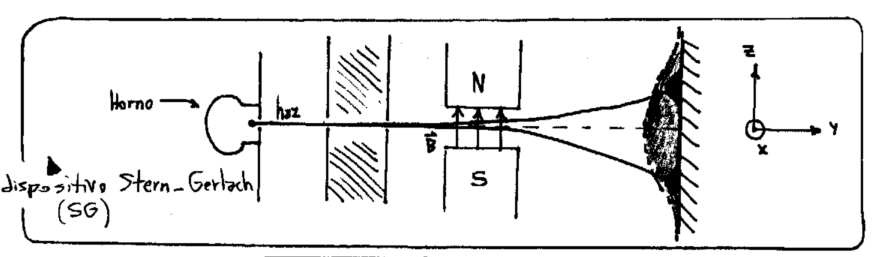
\includegraphics[width=0.8\textwidth]{images/teo2_1.pdf}	 
	\end{center}
	\caption{}
\end{figure} 

La fuerza $f_z$ que le ejerce el campo \vb{B} a estos átomos es 
\[
	f_z \propto - \mu_z
\]
de modo que el dispositivo SG mide y filtra por $S_z(\mu_z)$. Si el spín es un ente clásico
es de esperar un patrón como el sombreado en azul, pero se obtienen dos manchas; con la
correspondencia mostrada bajo estas líneas
\begin{figure}[htb]
	\begin{center}
	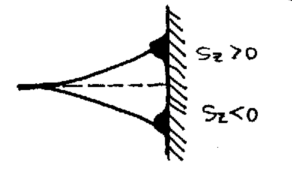
\includegraphics[width=0.4\textwidth]{images/teo2_2.pdf}	 
	\end{center}
	\caption{}
\end{figure} 

Entonces el spín no es un ente {\it continuo}: está cuantizado y sólo puede tomar dos valores.
Llamamos a estos estados
\[
	(S_z,+) \qquad \qquad (S_z,-)
\]
Luego, un aparato de SG filtra o selecciona ciertos átomos. Podemos combinarlos.

\begin{figure}[htb]
	\begin{center}
	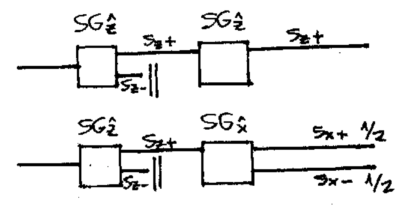
\includegraphics[width=0.6\textwidth]{images/teo2_3.pdf}	 
	\end{center}
	\caption{}
\end{figure} 

Con el dispositivo segundo orientado en $\hat{x}$ obtenemos mitad de átomos en
$(S_z,+)$ y mitad en $(S_z,-)$. La única es que en realidad lo que sucede es que 
$(S_z,+)$ se compone de $(S_x,+)$ y $(S_x,-)$.

Acá abajo sale $(S_z,-)$ pero para que ello sea posible 
$(S_x,+)$ se debe componer de $(S_z,+)$ y $(S_z,-)$. Pero esto no es posible
porque al segundo aparato no entró jamás $(S_z,-)$. Se filtró antes.

Los spines en $S_x, S_z$ son incompatibles. Al seleccionar $(S_z,+)$ en el segundo
SG se destruye la información previa sobre $S_z$. No podemos ya garantizar que $S_z$
sea nula.
El tercer experimento da al traste con la idea de que podamos pensar en spín como un
ente vectorial en 3D. Mediante una analogía con polarización de luz vemos que es necesario
meter al spín es un espacio vectorial de dimensión 2 pero con coeficientes complejos.

\begin{figure}[htb]
	\begin{center}
	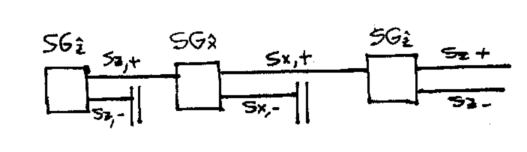
\includegraphics[width=0.6\textwidth]{images/teo2_4.pdf}	 
	\end{center}
	\caption{}
\end{figure} 

% =================================================================================================
\section{Algebra?}
% =================================================================================================

El ket contiene toda la información cuántica del estado. Da el estado físico del sistema.
\begin{itemize}
 \item $\Ket{\alpha} + \Ket{\beta}$ la suma de kets es un ket
 \item $c\Ket{\alpha}= \Ket{\alpha} c$ con $c\in\mathbb{C}$
 \item  $c_1\Ket{\alpha} + c_2\Ket{\beta} = \Ket{\gamma}$ con $c_1,c_2 \in \mathbb{C}$
 \item $c\Ket{\alpha},\Ket{\alpha}$ representan el mismo estado cuántico
\end{itemize}

Se define un espacio de {\it Bra} dual al de "kets" al que se va mediante ``dual conjugado''
\[
	\Ket{a}, \Ket{a'} \Leftrightarrow \Bra{a}, \Bra{a'}
\]
\[
	\Ket{a} + \Ket{b} \leftrightarrow \Bra{a} + \Bra{b} \qquad 
	c\Ket{a} \leftrightarrow c^*\Bra{a}
\]

Se define también un producto interno según
\[
	(\Bra{\alpha})(\Ket{\beta}) \equiv \Braket{\alpha|\beta}
\]
que no es otra cosa que un número complejo. Se puede hacer entonces una equivalencia con los vectores
estándard del álgebra del siguiente modo 
\[
	\text{ket} \sim \text{vector columna} \qquad \Ket{x} = \begin{pmatrix}
	                                                       1 \\
	                                                       0 \\
	                                                      \end{pmatrix}
\]
\[
	\text{bra} \sim \text{vector fila} \qquad \Bra{x} = ( 1 \; 0 )          
\]
y habiendo definido esta base escribimos, por ejemplo
\[
	\Ket{a} = \frac{1}{\sqrt{2}} \begin{pmatrix} 1 \\ 1  \\ \end{pmatrix}  =
	\frac{1}{\sqrt{2}} \begin{pmatrix} 1 \\ 0  \\ \end{pmatrix}  + 
	\frac{1}{\sqrt{2}} \begin{pmatrix} 0 \\ 1  \\ \end{pmatrix} =
	\frac{1}{\sqrt{2}} \Ket{x} + \frac{1}{\sqrt{2}} \Ket{y} 
\]
\[
	\Braket{a|x} = \frac{1}{\sqrt{2}}( 1 \; 1)\begin{pmatrix} 1 \\ 0  \\ \end{pmatrix} = \frac{1}{\sqrt{2}}
\]
y del mismo modo
\[
	\left( \frac{1}{\sqrt{2}} \Bra{x} + \frac{1}{\sqrt{2}} \Bra{y}  \right)
	\left( \Ket{x} \right)= \frac{1}{\sqrt{2}}
\]

\subsection{Propiedades}

\begin{enumerate}
 \item $\Braket{\beta|\alpha} = \Braket{\beta|\alpha}^*$ \text{luego} $ \Braket{\alpha|\alpha} \; \in \mathbb{R}$
 \item $\Braket{\alpha|\alpha} \geq 0$ \text{métrica definida positiva}
 \item $\Braket{\alpha|\beta} = \Braket{\beta|\alpha} = 0 \Leftrightarrow \Ket{\alpha} \perp \Ket{\beta}$
 \item $\Braket{\tilde{\alpha}|\tilde{\alpha}} = 1 \; \text{con} \; 
 \Ket{\tilde{\alpha}} = \frac{1}{\sqrt{\Braket{\alpha|\alpha}}}\Ket{\alpha} $ todo ket no nulo es normalizable
\end{enumerate}

\subsection{Operadores}

A cada observable lo representaremos por un operador. hay operaradores que no vienen de observables.
\[
	\hat{A}\Ket{\alpha} = \Ket{\gamma} \qquad \qquad  \Bra{\alpha} \hat{A} = \Bra{\gamma}
\]
un operador sobre un ket da otro ket y sobre un bra da otro bra. Notemos que en este último caso opera 
a izquierda. La transformación entre operadores se da con 
\[
	\hat{X}\Ket{a} \Leftrightarrow \Bra{a}\hat{X}^\dagger
\]
donde $\dagger$ (daga) significa el traspuesto conjugado; cambia el sentido hacia donde actúa el operador 
y conjuga. Se da que si 
\[
	\hat{X} = \hat{X}^\dagger \quad \Rightarrow \qquad \hat{X} \;\text{es hermítico}
\]
Se dan 
\begin{itemize}
 \item $\hat{X}\hat{Y} \neq \hat{Y}\hat{X} \qquad \qquad \text{no conmutativo}$
 \item $\hat{X}(\hat{Y}\hat{Z}) = (\hat{X}\hat{Y})\hat{Z} = \hat{X}\hat{Y}\hat{Z} \qquad \qquad \text{asociativo}$
 \item $(XY)^\dagger = Y^\dagger X^\dagger$
 \item $\hat{0}\Ket{\alpha} = 0 \qquad \forall \Ket{\alpha}$ ; $\hat{0} \equiv$ operador nulo
 \item $\hat{X}( c_1 \Ket{\alpha} + c_2 \Ket{\beta} ) = c_1 \hat{X}\Ket{\alpha} + c_2 \hat{X}\Ket{\beta} $
\end{itemize}

de modo que en cuántica los observables se representan mediante operadores hermíticos.

\subsection{sandwichs}

\[
	\Braket{\beta|X|\alpha} = (\Bra{\beta})(X\Ket{\alpha}) = \Braket{\beta|\gamma} =
	\Braket{\gamma|\beta}^* = (\Braket{\alpha|X|\beta})^*
\]
donde usamos que $\Ket{\gamma}$ es un ket y por dual conjugado $\Bra{\gamma} = \Bra{\alpha}\hat{X}^\dagger$ y
extraemos como conclusión 
\[
	\Braket{\beta|X|\alpha} = (\Braket{\alpha|X|\beta})^*
\]
y de manera equivalente
\[
	\Braket{\beta|X|\alpha} = (\Bra{\beta}X^\dagger)(\Ket{\alpha}) = \Braket{\Gamma|\alpha} =
	\Braket{\alpha|\Gamma}^* = (\Braket{\alpha|X^\dagger|\beta})^*
\]
donde usamos que $\Bra{\Gamma}$ es un bra y por dual conjugado $\Ket{\Gamma} = \hat{X}\Ket{\beta}$.
El formalismo parece ser consistente. El operador opera sobre un ket/bra y multiplica al otro.


\subsection{Producto externo}

\[
	\Ket{\beta} \Bra{\alpha} \equiv (\Ket{\beta} )( \Bra{\alpha} )
\]
\[
	( \Ket{\beta} \Bra{\alpha} )\Ket{\gamma} = \Ket{\beta} \Bra{\alpha} \Ket{\gamma} =
		\Braket{\alpha|\gamma} \Ket{\beta} , 
\]
de modo que es un operador pues al aplicar sobre un ket obtengo otro ket (notemos que $\Braket{\alpha|\gamma}$
es un escalar). Podemos pensar en que 
\[
	\Lambda_\alpha \equiv \Ket{\alpha}\Bra{\alpha}
\]
es el proyector, que actúa rotando un $\Ket{\gamma}$ en la dirección de $\Ket{\beta}$. Notemos 
\[
	\Lambda_\alpha^2 = \Ket{\alpha}\Bra{\alpha}\Ket{\alpha}\Bra{\alpha} = \Ket{\alpha}\Bra{\alpha} = \Lambda_\alpha
\]
puesto que $\Braket{\alpha|\alpha}=1$. El proyector $\Lambda_\alpha$ sobre un ket $\Ket{\beta}$ selecciona la parte de
$\Ket{\beta}$ en la dirección de $\Ket{\alpha}$. Nos dice cuanto de $\Ket{\beta}$ está en la dirección de 
$\Ket{\alpha}$.
Luego,
\[
	\sum_i^N \; \Lambda_i = \sum_i^N \; \Ket{i}\Bra{i} = \mathbb{1}
\]
la suma de todos los proyectores del espacio en el que estamos es la identidad de ese espacio. Decimos que $\Ket{i}$ es 
un conjunto completo. Se verifica además
\[
	(\Ket{\beta} \Bra{\alpha})^\dagger = \Ket{\alpha} \Bra{\beta}
\]
Algunas cuentitas de ejemplo en dos dimensiones,
\[
	\hat{X} = \begin{pmatrix} 1 \\ 0 \end{pmatrix} \qquad \qquad \hat{Y} = \begin{pmatrix} 0 \\ 1 \end{pmatrix}
\]
\[
	\hat{X}^\dagger = ( 1 \; 0 ) \qquad \qquad \hat{Y}^\dagger = ( 0 \; 1  ) 
\]
\[
	\hat{X}^\dagger\hat{X} = (1 \; 0) \begin{pmatrix} 1 \\ 0 \end{pmatrix} = 1 \qquad 
	\hat{X}\hat{X}^\dagger = \begin{pmatrix} 1 \\ 0 \end{pmatrix} (1 \; 0) = 
	\begin{pmatrix} 1 & 0 \\ 0 & 0 \\ \end{pmatrix},
\]
donde instamos al lector a que note la diferencia de dimensión en los resultados.

Los kets $\Ket{\alpha}$ {\it viven} en un espacio vectorial de Hilbert con dimensión N, donde N lo dicta el número de 
posibles estados de cada sistema físico. Una partícula de spín $1/2$ sólo tiene dos estados: up y down.
Hay otro producto más, que se llama producto tensorial y se representa como 
\[
	\Ket{\alpha} \otimes \Ket{\beta}
\]
que es un producto entre kets de espacios de Hilbert diferentes.
\[
	\Braket{\alpha|\beta}^* \equiv DC\{\ket{\beta}\} DC\{\Bra{\alpha}\}
\]

\section{Bases}

Dado un sistema físico representado por un espacio vectorial $\mathcal{H}$ de dimensión $N$ existirá una base (también 
de dimensión $N$) que será un conjunto de estados tal que cualquier estado de ese sistema físico puede representarse 
como combinación lineal de ese conjunto,
\[
	\{ \Ket{i}\} \; \text{base} \quad \Rightarrow \; \Ket{\alpha} = \sum_i^N c_i \Ket{i}
\]
siendo $\Ket{\alpha}$ un estado cualquiera.
Es práctico utilizar bases ortonormales,
\[
	\Braket{ i|j } = \delta_{ij} = \begin{cases}
	                                1 \quad i=j \\
	                                0 \quad i\neq j
	                               \end{cases}
\]
que es la delta de Kronecker.

Así, los kets se definen normalizados.
\[
	\Ket{\psi} = a \Ket{1} + b \Ket{2} + c \Ket{3} + d \Ket{4} \qquad\quad |a|^2 + |b|^2 +|c|^2 +|d|^2 = 1
\]
sea $\Ket{\phi} = a \Ket{1} + b \Ket{2}$, $\Bra{\phi} = a^*\Bra{1} + b^* \Bra{2}$ entonces 
\[
	\Braket{\phi|\phi} = (a^*\Bra{1} + b^* \Bra{2})(a \Ket{1} + b \Ket{2}) = 
	a^*a \Braket{1|1} + b^*a\Braket{2|1} + a^*b\Braket{1|2} + b^*b\Braket{2|2} =
	|a|^2 + |b|^2 = 1
\]

\subsection{Autokets y autovalores}

Si $\hat{A}\Ket{a}=c\Ket{a}$ entonces $\Ket{a}$ es autoket de $\hat{A}$ con autovalor $c$. Se suelen 
etiquetar los autoestados $\Ket{a'}, \Ket{a''}$ de modo que 
\[
	\hat{A}\Ket{a'} = a'\Ket{a'}
\]
lo cual lleva al problema espectral
\[
	\left(\hat{A} - a'\mathbb{1}\right) \Ket{a'} = 0
\]
entonces los operadores tendrán representación matricial, que cambiará según la base utilizada.ñ
Vamos viendo que en general sólo se sabe cómo opera un operador sobre kets. La operación sobre los
bras la obtenemos usando dual conjugado.

Deducimos entonces que
\begin{enumerate}
 \item Los autovalores de un operador hermítico son reales y los autokets correspondientes a diferentes
 autovalores son ortogonales.
 \item Los autokets de un operador son base completa del espacio de kets.
\end{enumerate}

Como ejemplo de A citemos
\[
	a'\Ket{a'} = A\Ket{a'} \quad \text{DC} \quad \Bra{a'} A^{\dagger} = \Bra{a'} A = \Bra{a'}a'^*
\]
de manera que 
\[
	\Braket{a'|A|a'} = ( \Bra{a'} )( A\Ket{|a'} ) = a'
\]
\[
	( \Braket{a'|A|a'} )^* = ( \Bra{a'} )( A\Ket{|a'} )^* = ( \Bra{|a'}A^\dagger )( \Ket{a'} )
\]
\[
	= \Braket{a'|A|a'} = a' \qquad \Rightarrow \quad a' = a'^*.
\]

Para el caso de B se postula así. Si esto vale entonces 
\[
	\Ket{\alpha} = \sum_i^N \Ket{a_i}\Bra{a_i} \Ket{\alpha} = \sum_i^N c_i \Ket{a_i} = 
	\mathbb{1}\Ket{\alpha}
\]
pues 
\[
	\Braket{\alpha|\alpha} = \sum_{i,j}^N \Braket{ a_j|c_j^* c_i|a_i} = \sum_i^N |c_i|^2 = 1
\]
y además 
\[
	A\Ket{a'} = a'\Ket{a'} \qquad A\Ket{a''} = a''\Ket{a''} \Rightarrow 
	A(\Ket{a'} - \Ket{a''} ) = a'\Ket{a'} - a''\Ket{a''}
\]
\[
	\Braket{ a''|A|a' } = a' \Braket{ a''|a' } \qquad \Braket{ a'|A|a'' } = a'' \Braket{ a'|a'' }
\]
y ahora conjugando
\[
	\Braket{ a''|A|a' }^* = a' \Braket{ a''|a' }^* \qquad \Braket{ a''|A|a' } = a'' \Braket{ a''|a' }
\]
donde usamos que $a''^* = a''$ y restando 
\[
	(a'-a'')\Braket{a''|a'} = 0 \qquad \Rightarrow \; \Braket{a''|a'} = 0 
		\quad \text{si} \quad a'\neq a''
\]
Si la base es completa entonces es $\sum \Lambda = 1$.

\subsection{Operadores y matrices}

Un operador se puede representar matricialmente como 
\[
	X = \sum_{a'}^N  \sum_{a''}^N \Ket{a''} \Bra{a''} X \Ket{a'} \Bra{a'} =  
	\sum_{a'}^N  \sum_{a''}^N ( \Braket{a''|X|a'} ) \Ket{a''} \Bra{a'}
\]
donde hemos explotado el hecho de que en el medio aparece un escalar (?), siendo 
\[
	X_{ij} = \Braket{a_i|X|a_j}
\]
un elemento de matriz. Y notemos que $\Ket{a''} \Bra{a'}$ es un ente de $N\times N$.
Si la base es de dimensión 3 se tendrá por ejemplo,
\[
	X = \begin{pmatrix}
	 x_{11} & x_{12} & x_{13} \\
	 x_{21} & x_{22} & x_{23} \\
	 x_{31} & x_{32} & x_{33} \\
	\end{pmatrix}
\]
de manera que existe una identificación entre cosas del álgebra básica y este mundo
de operadores y estados.
Si $X$ es hermítico por ejemplo, entonces su matriz es simétrica conjugada.
\[
	\Braket{a_i|X|a_j}^* = (\Bra{a_j}X^\dagger)(\Ket{a_i}) = \Braket{a_j|X|a_i}
\]
y entonces 
\[
	\Braket{a_j|X|a_i}^* = \Braket{a_i|X|a_j}
\]
de modo que 
\[
	X_{ji}^* = X_{ij} \qquad X_{ij}^{t*} = X_{ij} \qquad X_{ij}^\dagger=X_{ij}
\]
y vemos bien el significado de {\it daguear}. En este caso la matriz tiene traza real
y seis elementos independientes
\[
	X = \begin{pmatrix}
	  X_{11} & X_{12} & X_{13} \\
	  X_{12}^* & X_{22} & X_{23} \\
	  X_{13}^* & X_{23}^* & X_{33} \\
	\end{pmatrix} =
	\begin{pmatrix}
	  X_{11} & X_{12} & X_{13} \\
	  X_{21} & X_{22} & X_{23} \\
	  X_{31} & X_{32} & X_{33} \\
	\end{pmatrix} =
	\begin{pmatrix}
	  X_{11}^* & X_{21}^* & X_{31}^* \\
	  X_{12}^* & X_{22}^* & X_{32}^* \\
	  X_{13}^* & X_{12}^* & X_{33}^* \\
	\end{pmatrix}
\]

\subsection{Combinación lineal de autoestados}

Un estado $\Ket{\alpha}$ se puede escribir en función de la base $\Ket{a_i}$ de esta forma 
\[
	\Ket{\alpha} = \sum_{i=1}^N \Ket{a_i}\Braket{a_i|\alpha} = 
		\sum_{i=1}^N (\Braket{a_i|\alpha}) \Ket{a_i}
\]
y entonces
\[
	\Braket{a_i|\alpha} = \sum_{i=1}^N c_i \underbrace{\Braket{a_j|a_i}}_{\delta_{ij}} = c_j 
\]

\subsection{Cambio de base}

Para cambiar de base metemos un uno ($\mathbb{1}$) escrito como suma de proyectores,
\[
	X\Ket{b_j} = \sum_{i=1}^N \Ket{a_i}\Braket{a_i|X|b_j} = \sum_{i=1}^N C_{ij} \Ket{a_i}
\]
siendo $C_{ij}$ la matriz del cambio de base.
Se puede escribir
\[
	\Ket{b_j} = \sum_{i=1}^N \Ket{a_i}\Braket{a_i|b_j} 
\]
y se ve que $\Braket{a_i|b_j}$ son los elementos de la matriz que cambia de base.

\subsection{Representación diagonal}

Un operador tiene representación diagonal cuando está representado en la base de sus
autokets
\[
	A = \sum_i^N\sum_j^N \Ket{a_i}\Braket{a_i|A|a_j}\Bra{a_j} =
		\sum_i^N\sum_j^N a_j\Ket{a_i}\Braket{a_i|a_j}\Bra{a_j} =
		\sum_{i,j}^N \delta_{ij} a_j \Ket{a_i}\Bra{a_j} = \sum_i^N a_i \mathbb{1}
\]
\[
	A = \begin{pmatrix} 
		a_1 & 0 & ... & 0 \\
		0 & a_2 & ... & 0 \\
		0 & 0 & ... & 0 \\
		0 & 0 & ... & a_n \\
	\end{pmatrix}
\]
y $a_1,a_2,...,a_n$ son sus autovalores.
Es destacable que es conveniente utilizar como bases los autoestados de ciertos operadores.

\subsection{Representaciones canónicas}

Podemos representar una base como vectores canónicos
\[
	\Ket{a_1} = \begin{pmatrix}
			1 \\
			0 \\
			. \\
			. \\
			N
			\end{pmatrix} \qquad 
	\Ket{a_1} = \begin{pmatrix}
			0 \\
			1 \\
			. \\
			. \\
			N
			\end{pmatrix} \qquad 
	\Ket{a_n} = \begin{pmatrix}
			0 \\
			0 \\
			. \\
			. \\
			1
			\end{pmatrix}
\]
luego 
\[
	\Ket{\alpha} = \sum_i \Ket{a_i}\Braket{a_i|\alpha} =
		\Braket{a_1|\alpha} \begin{pmatrix}
			1 \\
			0 \\
			. \\
			. \\
			N
			\end{pmatrix} +
		\Braket{a_2|\alpha} \begin{pmatrix}
			0 \\
			1 \\
			. \\
			. \\
			N
			\end{pmatrix} +
			... +
		\Braket{a_n|\alpha} \begin{pmatrix}
			0 \\
			0 \\
			. \\
			. \\
			1
			\end{pmatrix} =
\]
\[
	\begin{pmatrix}
		\Braket{a_1|\alpha} \\
		\Braket{a_2|\alpha} \\
			... \\
			... \\
		\Braket{a_n|\alpha}
	\end{pmatrix}
\]
y por DC se tiene 
\[
	\Bra{\alpha} = ( \Braket{\alpha|a_1} \Braket{\alpha|a_2} ... \Braket{\alpha|a_n} )
\]
y 
\[
	\Braket{\alpha|\alpha} = 1 = \overbrace{( \phantom{1} \qquad \phantom{1} )}^{1\times 
N}\overbrace{\begin{pmatrix} \phantom{1} \\ 	\phantom{1}  \end{pmatrix} }^{N\times 1} = \Box
\]
que es un escalar.
\[
	\Braket{\beta|\alpha} = \Braket{\beta|a_i} \Braket{a_i|\alpha} = 
	\sum_i^N \Bra{\beta} \underbrace{\Ket{a_i} \Braket{a_i}}^{\Lambda_{a_i}} \Ket{\alpha} = \Box 
\]
otra vez un escalar.
\[
	\Braket{a_i|\gamma} = \Braket{a_i|X|\alpha} = \sum_{a_j} \Braket{a_i|X|a_j}\Braket{a_j|\alpha}
\]
\[
	\begin{pmatrix}
	 \Braket{a_1|\gamma} \\
	 ... \\
	 ... \\
	\end{pmatrix} = 
	\begin{pmatrix}
	 X_{11} & X_{12} & ...\\
	 X_{21} & X_{22} & ... \\
	 ... \\
	\end{pmatrix}
	\begin{pmatrix}
	 \Braket{a_1|\alpha} \\
	 ... \\
	 ... \\	 
	\end{pmatrix}
\]
\[
	X = \sum_i^N \sum_j^N \Ket{a_i} \Braket{a_i|X|a_j} \Bra{a_j} =
		\sum_i^N \sum_j^N  \Braket{a_i|X|a_j} \Ket{a_i} \Bra{a_j}
\]
y esto último es una matriz. Aquí el $\hat{X}$ es una matriz y $\Braket{a_i|\hat{X}|a_j} \equiv X_{ij}$ son 
sus elementillos (escalares).

\section{Sistemas de spín 1/2}

Hay dos estados posibles de spin $(\Ket{+}, \Ket{-})$ entonces dimensión del espacio vectorial es 2. De 
manera que 
\[
	\mathbb{1} = \Ket{+}\Bra{+} \; + \;  \Ket{-}\Bra{-}
\]
\[
	\Ket{S_z ; +} = \Ket{S_z = \hbar/2} \equiv \Bra{+} 
\]
\[
	\Ket{S_z ; -} = \Ket{S_z = -\hbar/2} \equiv \Bra{-}
\]
\notamargen{Acá hay que diseñar unos $+,-$ que habiten dentro de los brakets pues estos se ven feo.}

Tenemos operadores de subida y de bajada,
\[
	S_+ = \hbar \Ket{+}\Bra{-} \qquad S_- = \hbar \Ket{-}\Bra{+}
\]
que actúan subiendo el spin o dando el ket nulo,
\[
	S_+ = \hbar \begin{pmatrix} 1 \\ 0 \end{pmatrix} ( 0 \; 1 ) 
		= \hbar \begin{pmatrix}  0 & 1 \\ 0 & 0 \end{pmatrix}
\]
o bien bajando el spín o dando el ket nulo,
\[
	S_- =\hbar \hbar \begin{pmatrix} 0 \\ 1 \end{pmatrix} ( 1 \; 0 ) 
	 = \hbar \begin{pmatrix} 0 & 0 \\ 1 & 0 \end{pmatrix}
\]

\subsection{Cambio de base}

Dados dos conjuntos base ortonormales y completos existe un $\widehat{U}$ unitario tal que 
\[
	U^+U=UU^+=\mathbb{1} \qquad \Ket{b_i}=U\Ket{a_i}
\]

Este operador de cambio de base será 
\[
	U = \sum_\ell \Ket{b_\ell}\Bra{a_\ell}
\]
\[
	U\Ket{a_i} = \sum_\ell \Ket{b_\ell}\Braket{a_\ell|a_i} = \Ket{b_i}
\]
que tiene por función pasar 
\[
	\underbrace{\Ket{a_\ell}}_{\text{vieja base}} \longrightarrow \underbrace{\Ket{b_\ell}}_{\text{nueva base}}
\]
\[
	\Braket{b_k|\alpha} = \sum_\ell \Braket{b_k|a_\ell}  \Braket{a_\ell|\alpha}  =
	\sum_\ell \Braket{a_k|U^+|a_\ell}  \Braket{a_\ell|\alpha} = \Braket{a_k|U^+|\alpha} 
\]

Entonces
\[
	\Ket{\text{nueva base}} = U \Ket{\text{vieja base}}
\]
\[
	\Braket{b_i | x | b_j} = \sum_{\ell,m} \Braket{b_i|a_\ell}\Braket{a_\ell|x|a_m}\Braket{a_m|b_j }
\]
\[
	\Braket{b_i | x | b_j} = \sum_{\ell,m}\Braket{a_i|U^+|a_\ell}\Braket{a_\ell|x|a_m}\Braket{a_m|U|a_j}
\]
\[
	X_{\Ket{b}} = U^+ X_{\Ket{a}} U,
\]
que es una transformación de similaridad.

\subsection{Mediciones y probabilidades}

En mecánica cuántica medir es filtrar. La medición perturba al sistema. Se miden variables dinámicas asociadas a 
observables.
Como los autoestados de un observable $\hat{A}$ son una base completa $\{\Ket{a_i}\}$ entonces un sistema se hallará en 
una combinación lineal de autoestados de $\hat{A}$, o al menos eso puede pensarse.


\begin{tabular}{|c|c|c|}
\hline
antes de medir & & luego de medir \\
\hline 
sistema en CL
de autestados de $\hat{A}$ & Medición de $\hat{A}$ & Salta a un autoestado de $\hat{A}$ \\
\hline 
sistema en 
autoestado de $\hat{A}$  & & Continúa en autoestado de $\hat{A}$ \\
\hline
\end{tabular}

Puede verse pictóricamente la medición así:
\[
	\Ket{\alpha} \longrightarrow \Ket{a'}
\]
el proceso de medición hace saltar hacia $\Ket{a'}$ siendo el resultado de la medida el autovalor $a'$.
Luego,
\[
	\mathrm{Prob}_{\Ket{a'}} \equiv |\Braket{a'|\alpha}|^2
\]

Antes de medir no puedo saber a qué estado saltará y tampoco en qué estado se hallaba. Si $P=1$ se halla en
$\Ket{a'}$ antes de saltar, si $P=0$ no se halla en $\Ket{a'}$ antes de saltar.

\subsection{Valor de expectación}

\[
	\Braket{\widehat{A}} \equiv \Braket{\alpha|A|\alpha}
\]c
el valor de expectación siempre se refiere a un estado en particular.
\[
	\Braket{A} = \sum_{a',a''} \Braket{\alpha|a'}	\Braket{a'|A|a''} \Braket{a''|\alpha}
\]
\[
	\Braket{A} = \sum_{a',a''}  \Braket{\alpha|a'} a''\delta_{a'a''} \Braket{a''|\alpha} =
			\sum_{a''} a''|\Braket{\alpha|a''}|^2
\]
\[
	\Braket{A} = \sum_{a',a''} = a'' \text{Prob}_{\Ket{a''}}
\]
Esto último tiene el sentido de una especie de promedio ponderado.


\subsection{Conmutadores}

Se definen, el conmutador
\[
	[ A, B] \equiv AB - BA,
\]
y el anticonmutador
\[
	\{ A, B \} \equiv AB + BA,
\]
y se dice que dos observables conmutan si $[A,B]=0$. Se dice que son compatibles si $[A,B]=0$ y anticompatibles si se 
da la contrario, $[A,B]\neq 0$.

TEOREMA:

Sean dos observables compatibles y no degenerados, entonces los autoestados $\{ \Ket{a'}\}$ de $A$ lo son también de 
$B$. Es decir que A y B tienen base de autoestados en común.

demostración:
\[
	\Braket{a'|AB-BA|a''} = 0 
\]
\[
	a' \Braket{a'|B|a''} - \Braket{a'|B|a''} a''= (a'-a'') \Braket{a'|B|a''}= 0 
\]
entonces 
\[
	\Braket{a'|B|a''} = 0
\]
y $B$ es diagonal en $\{ \Ket{a'}\}$.

Los autoestados son iguales pero no los autovalores; con lo cual se utilizará la notación $\Ket{a',b'}$ donde 
\[
	A \Ket{a',b'} = a' \Ket{a',b'} \qquad \qquad B \Ket{a',b'} = b' \Ket{a',b'}
\]

\subsection{Degeneración}

Puede darse que haya varios $g$ autoestados correspondientes a un mismo autovalor $a'$; entonces se dice que hay 
degeneración de orden $g$ para el autoestado $\Ket{a'}$
\[
	A\Ket{a'}= a'\Ket{a'} \quad ; i=1,2,...,g
\]
y $A$ tendrá una matriz de $m\times n$ bloques. 
En este caso no se puede decir que la base de $A$ diagonalice a $B$.\notamargen{Mejorar la matriz que está un asco}
\[
	A = \begin{pmatrix}
	     a'\mathbb{1} & 0 & & \\
	     0 & a''\mathbb{1} & & \\
	     & & a'''& \\
	     & & & a^IV \\
	     ...
	    \end{pmatrix}
\]
Los $\ket{a'_i}$ no dan información sobre los bloques correspondientes en la matriz de $B$.
Necesito un conjunto de operadores que haga romper la degeneración para expresar unívocamente 
el estado del sistema. Se llama CCOC. Necesito que conmuten entre sí para que las mediciones tengan sentido.

Si no conmutan entonces son incompatibles; la medición de uno hace saltar al sistema a un autoestado del otro y como no 
son comunes pierde sentido el concepto de medir. No tiene sentido la medición de algo si por el hecho de medir 
cambiamos lo que queremos medir.
Al ser incompatibles sus mediciones de afectan mutuamente.

Los autovalores de algunos operadores podrán tener degeneración pero una combinación de los autovalores del CCOC, 
$\Ket{a'b'c'...}$, determina el estado de forma única.

Dado un set CCOC, $\{A,B,C,D\}$, se etiquetarán $\Ket{K'} \equiv \Ket{a'b'c'd'}$ los autoestados.
Las únicas cosas que tiene sentido medir en MC son las variables asociadas a operadores en un CCOC.

Sean $A,B$ compatibles sin degeneración
\[
	\Ket{\alpha} \overbrace{\underbrace{\longrightarrow}_{a'}}^{\text{Mido A}} \Ket{a'b'}
	\overbrace{\underbrace{\longrightarrow}_{b'}}^{\text{Mido B}} \Ket{a'b'} 
	\overbrace{\underbrace{\longrightarrow}_{a'}}^{\text{Mido A}} \Ket{a'b'}
\]
En cambio si $A,B$ son compatibles pero con degeneración 
\[
	\Ket{\alpha} \overbrace{\underbrace{\longrightarrow}_{a'}}^{\text{Mido A}} 
		\sum_{i=1}^g C_{a'}^{(i)}\Ket{a'b'(i)} \overbrace{\underbrace{\longrightarrow}_{b'(j)}}^{\text{Mido B}} 
		C_{a'}^{(j)}\Ket{a'b'(j)} \overbrace{\underbrace{\longrightarrow}_{a'(j)}}^{\text{Mido A}} 
		C_{a'}^{(j)} \Ket{a'b'(j)}
\]

Al medir A y obtener $a'$ no tengo determinado el estado del sistema. Me hallaré en una CL de autoestados 
correspondientes al autovalor degenerado $a'$. Al medir luego B selecciono uno de los $\Ket{a'b'}$ degenerados, el 
correspondiente a $b'(j)$ pues B no está degenerado. Puedo volver a medir A pues el autoestado en que ha caído el 
sistema permanece incólume.


\subsection{Postulados de la mecánica cuántica}

\begin{enumerate}
 \item El estado de un sistema lo definimos con un ket $\Ket{\alpha} \in \mathcal{H}$ y con $\Braket{\alpha|\alpha}=1$
 \item Asociamos a propiedades físicas (observables) operadores hermíticos $\widehat{A}$ que operan sobre los ketes. 
	Los autokets $\Ket{a}$ verifican :
\[
	\widehat{A}\Ket{a} = a \Ket{a}, 
\]
y $\{ \Ket{a} \}$ es base del espacio de kets.
 \item Al medir una cantidad física representada por el observable $\widehat{A}$ obtenemos un autovalor $a'$.
 Luego de medir, el estado del sistema es $\Ket{a'}$.
 \[
	\Ket{\Psi} \overbrace{\underbrace{\longrightarrow}_{a'}}^{\text{Mido A}} \Ket{\Psi'} =
	\Ket{a}\Bra{a}\Ket{\Psi} =(\Braket{a|\Psi})\Ket{a}
 \]
 hecho al sistema a un autoestado de $\widehat{A}$. Quizás deba ahora normalizar. $\Braket{\Psi|\Psi}=1$
 El esquema de arriba representa la frase ``proyectar sobre la base de autoestados''.
 \item Las transformaciones espaciales se generan por $\vb{p}$
 \[	
	[x_i,p_j] = i\hbar\delta_{ij}
 \]
 \item La evolución temporal la realiza $H$ (el hamiltoniano).
\end{enumerate}

\notamargen{Extrañamente el punto 4 estaba vacío. Raro.}

\subsection{Operador de dispersión}

\[
	\Delta \widehat{A} \equiv \widehat{A} - \Braket{A}\mathbb{1}
\]
la dispersión será nula en un autoestados del operador $\widehat{A}$. Luego la dispersión cualitativamente nos dice 
``qué tan lejos'' del autoestado nos hallamos.
\[
	\Braket{(\Delta A)^2} = \Braket{(\widehat{A} - \Braket{A}\mathbb{1})^2} =
	\Braket{ A^2 - 2A\Braket{A} + \Braket{A}^2 } = \Braket{A^2} - 2A\Braket{A}^2 + \Braket{A}^2 =
	\Braket{A^2} - \Braket{A}^2
\]
y la relación de dispersión generalizada
\[
	\Braket{(\Delta A)^2} \Braket{(\Delta B)^2} \geq \frac{1}{4}|\Braket{[ A,B ]}|^2
\]

\subsection{Espectro continuo}

Hay observables con espectro de autovalores continuo.
Nos podemos construir la siguiente tabla para comparar ambos escenarios.

\begin{tabular}{|c|c|}
\hline 
Espectro discreto & Espectro continuo \\
\hline
  & \\
  $A\Ket{a'}=a'\ket{a'}$ & $Y\Ket{y'}=y'\ket{y'}$ \\
  & \\
  $\mathbb{1} = \sum_{a' }^N \Ket{a'}\Bra{a'} $ & $\mathbb{1} = \int_{-\infty}^ {\infty} \Ket{y'}\Bra{y'} dy' $ \\
  & \\
  $\Braket{a'|a''} = \delta_{a' a''}$ & $\Braket{y'|y''} = \delta(y'-y'')$ \\
  & \\
  $ \sum_{a' }^N \Braket{a'|a''}\Bra{a''} = \Bra{a'}$ & $ \int_{-\infty}^\infty dy'' \Braket{y'|y''}\Bra{y''} = 
\Bra{y'}$ \\
  & \\
  $ \sum_{a' }^N \Ket{a'} \Braket{a'|\alpha} =  \Ket{\alpha}$ & $ \int_{-\infty}^\infty dy' \Ket{y'}\Braket{y'|\alpha} 
= \Ket{\alpha}$ \\
  & \\
  $ \sum_{a' }^N |\Braket{a'|\alpha}|^2 = 1$ & $ \int_{-\infty}^\infty dy'|\Braket{y'|\alpha}|^2 = 
1$ \\
  & \\
    $ \Braket{\beta | \alpha}  = \sum_{a' }^N \Braket{\beta|a'}\Braket{a'\alpha}$ & $ \Braket{\beta | \alpha}  = 
\int_{-\infty}^\infty dy' \Braket{\beta|y'}\Braket{y'\alpha}$ \\
  & \\
\hline  
\end{tabular} 

\subsection{La función de onda}

\[
	\Ket{\alpha} = \int_{\infty}^\infty dx' \Ket{x'}\Braket{x'|\alpha}
\]
donde 
\[
	\Braket{x'|\alpha}dx'
\]
es la densidad de probabilidad y 
\[
	|\Braket{x'|\alpha}|^2
\]
es la amplitud de probabilidad. La densidad de probabilidad, en el formalismo de Schrödinger, es la función de onda
\[
	\Psi_\alpha(x) = \Braket{x|\alpha}
\]
siendo este el vínculo entre la representación de Dirac y la función de onda,
\[
	\Braket{\beta|\alpha} = \int dx' \Braket{\beta|x'}\Braket{x'|\alpha} = 
		\int dx' \Psi_\beta^*(x) \Psi_\alpha(x)
\]
\[
	\Braket{\beta|A|\alpha} = \int \int dx' dx''\Braket{\beta|x''}\Braket{x''|A|x'}\Braket{x'|\alpha}
\]
\[
	\Braket{\beta|A|\alpha} = \int \int dx' dx'' \Psi_\beta^*(x'') \Braket{x''|A|x'} \Psi_\alpha(x')
\]
y si $A=f(\hat{x})$ entonces $f(\hat{x}) \Ket{x'} = f(x') \Ket{x'}$ y
\[
	\Braket{\beta|A|\alpha} = \int \int dx' dx'' \Psi_\beta^*(x'') f(x')\delta(x''-x') \Psi_\alpha(x')
\]
y entonces 
\[
	\Braket{\beta|A|\alpha} = \int dx' \Psi_\beta^*(x') f(x') \Psi_\alpha(x').
\]

En forma análoga tenemos la representación de momento;
\[
	\hat{p}\Ket{p'} = p'\Ket{p'} \qquad \Braket{p'|p''} = \delta(p'-p'') \qquad 
	\Ket{\alpha} = \int dp' \Ket{p'}\Braket{p'|\alpha}
\]
\[
	\Phi_\alpha(p') = \Braket{p'|\alpha}.
\]

\subsection{Operador de traslación}

Se le pedirá
\[
	\Tau_{(dx')} \Ket{x'} = \Ket{x'+dx'}
\]
siendo este requerimiento intuitivamente adecuado para una traslación. Nótese que $dx'$ no es un operador, es el 
parámetro de la traslación.

Cumplirá las propiedades
\begin{itemize}
 \item Unitariedad:
 \[
	\Tau^\dagger\Tau = \Tau \Tau^\dagger = \mathbb{1}
 \]
 para que no varíe la probabilidad ante un cambio de coordenadas.
 \item Aditividad:
 \[
	\Tau_{(dx')}\Tau_{(dx'')} = \Tau_{(dx'+dx'')}
 \]
 porque vale en mecánica clásica.
 \item Existencia de inverso:
 \[
	\Tau_{(dx')}^{-1} = \Tau_{(-dx'')}
 \]
 \item Límite a $\mathbb{1}$
 \[
	\Tau_{(dx')} \to \mathbb{1} \quad \text{si} \quad dx' \to 0
 \]
\end{itemize}

Se propone un 
\[
	\Tau_{(dx')} = \mathbb{1} - i \vb{K}\cdot d\vb{x}'
\]
con $\vb{K}$ hermítico (notemos que $\tau$ no es hermítico). Comparando con mecánica clásica vemos que \vb{p} origina 
las traslaciones, entonces identificamos $K$ con $p$.
\notamargen{Hay que ver el carácter vectorial de estas cosas.}

Entonces pedimos que \vb{p} cuántico origine las traslaciones
\[
	\vb{K} = \frac{\vb{p}}{\hbar} \qquad \Tau_{(dx')} = \mathbb{1} - \frac{i}{\hbar} \vb{P}\cdot d\vb{x}'
\]
y así
\[
	\Tau_{(dx')}\Ket{p'} = \left( \mathbb{1} - \frac{i}{\hbar} \vb{P}\cdot d\vb{x}' \right)\Ket{p'} =
	\left( 1 - \frac{i}{\hbar} p' dx \right)\Ket{p'}
\]
el autovalor no es real, pues $\Tau$ no es hermítico.

Partiendo del conmutador 
\[
	x \Tau_{(dx')} - \Tau_{(dx')} x = dx \Tau_{(dx')}
\]
entonces 
\[
	[x, \Tau_{(dx')}] = dx\Tau 
\]
y con $dx\sim 0$ a orden uno (esto significa que tiramos los términos cuadráticos en $dx$)
\[
	[ x, p_x ] = i \hbar
\]
se llega a la incompatibilidad de posición y momento, generalizando
\[
	[ x_i, p_j ] = i \hbar \delta_{ij}
\]
Pero las traslaciones en diferentes direcciones conmutan
\[
	[ \Tau_{(d\vb{x}')}, \Tau_{(d\vb{x}'')} ] = 0  \qquad [ p_i, p_j ] = 0
\]

Sumando infinitas traslaciones infinitesimales tenemos una traslación finita,
\[
	\Tau_{(\Delta x')} = \lim_{N\to \infty}\left( 1 - \frac{i}{\hbar}p\frac{\Delta x'}{N}\right)^N 
		= \euler^{-i/\hbar \: p\Delta x'}
\]
y entonces 
\[
	\Tau_{(\Delta x')} = \euler^{-i/\hbar\: \vb{p}\cdot\Delta \vb{x}'}
\]


\subsection{\vb{p} en la representación \vb{x}}

\[
	\Tau_{(\Delta x)} \Ket{\alpha} = \int dt' \Tau\Ket{x'}\Braket{x'|\alpha} = 
		\int dt' \Ket{x'+ \Delta x}\Braket{x'|\alpha} = \int dt' \Ket{x'}\Braket{x'-\Delta x|\alpha}
\]
pero
\[
	\dpar{}{x'} \Braket{x'|\alpha} \approx \frac{ -\Braket{x'-\Delta x|\alpha} + \Braket{x'|\alpha} }{\Delta x}
\]
y entonces
\[
	-\dpar{}{x'} \Braket{x'|\alpha} \Delta x + \Braket{x'|\alpha}  = \Braket{x'-\Delta x|\alpha}
\]

\[
	\Tau\Ket{\alpha} = \int dx' \Ket{x'}\left( \Braket{x'|\alpha} -\dpar{}{x'} \Braket{x'|\alpha} \Delta x \right) =
	\int dx' \Ket{x'} \Braket{x'|\alpha} - \int dx' \Ket{x'}  \dpar{}{x'} \Braket{x'|\alpha} \Delta x 
\]
\[
	\left( 1 - \frac{i}{\hbar}p\Delta x \right) \Ket{\alpha} = 
		\Ket{\alpha} - \int dx' \Ket{x'}  \dpar{}{x'} \Braket{x'|\alpha} \Delta x
\]
\[
	\frac{i}{\hbar}p\Delta x \Ket{\alpha} = \int dx' \Ket{x'}  \dpar{}{x'} \Braket{x'|\alpha} \Delta x
\]
y así
\[
	p\Ket{\alpha} = -i\hbar \int dx' \Ket{x'}  \dpar{}{x'} \Braket{x'|\alpha}
\]
de modo que usándo este resultado se tienen
\[
	\Braket{x''|p|\alpha} = -i\hbar \int dx' \Braket{x''|x'}  \dpar{}{x'} \Braket{x'|\alpha}
\]
\[
	\Braket{x''|p|\alpha} = -i\hbar \dpar{}{x'} \Braket{x''|\alpha}
\]
\[
	\Braket{\beta|p|\alpha} = \int dx' \Braket{\beta|x'} (-i\hbar) \dpar{}{x'} \Braket{x'|\alpha}
\]
\[
	\Braket{\beta|p|\alpha} = \int dx' \Psi_\beta^*(x') (-i\hbar) \dpar{}{x'} \Psi_\alpha(x')
\]
de lo que se deduce 
\[
	\hat{p} \equiv - i \hbar \dpar{}{x},
\]
que es el resultado más importante de la sección.

% \bibliographystyle{CBFT-apa-good}	% (uses file "apa-good.bst")
% \bibliography{CBFT.Referencias} % La base de datos bibliográfica

\end{document}

	
		\documentclass[10pt,oneside]{CBFT_book}
	% Algunos paquetes
	\usepackage{amssymb}
	\usepackage{amsmath}
	\usepackage{graphicx}
	\usepackage{libertine}
	\usepackage[bold-style=TeX]{unicode-math}
	\usepackage{lipsum}

	\usepackage{natbib}
	\setcitestyle{square}

	\usepackage{polyglossia}
	\setdefaultlanguage{spanish}
	



	\usepackage{CBFT.estilo} % Cargo la hoja de estilo

	% Tipografías
	% \setromanfont[Mapping=tex-text]{Linux Libertine O}
	% \setsansfont[Mapping=tex-text]{DejaVu Sans}
	% \setmonofont[Mapping=tex-text]{DejaVu Sans Mono}

	%===================================================================
	%	DOCUMENTO PROPIAMENTE DICHO
	%===================================================================

\begin{document}

% =================================================================================================
\chapter{Dinámica cuántica}
% =================================================================================================

Queremos ver la evolución temporal de los kets 
\[
	\Ket{\alpha,t_0,t},
\]
notación que refiere al estado $\alpha$ que partió en $t_0$ al tiempo $t$. Pictóricamente
\[
	\Ket{\alpha,t_0} \underbrace{\longrightarrow}_{\text{evoluciona}} \Ket{\alpha,t_0,t}
\]

Emplearemos para ello un operador de evolución temporal $U_{(t,t_0)}$ al cual le pediremos
\[
	\Ket{\alpha,t_0,t} = U \Ket{\alpha,t_0}
\]
con las propiedades

\begin{itemize}
 \item Unitariedad
 \[
	\Braket{ \alpha,t_0,t| \alpha,t_0,t} = 1 \forall t
 \]
 \[
	\Braket{ \alpha,t_0| U^\dagger U| \alpha,t_0} = 1 \quad \Rightarrow \quad 
	U^\dagger U = U U^\dagger = \mathbb{1}
 \]
 para conservación de la probabilidad.
 \item Linealidad
 \[
	U(t_2,t_0) = U(t_2,t_1) U(t_1,t_0) \qquad t_2>t_1>t_0
 \]
 \item Límite a $\mathbb{1}$
 \[
	U_{(t,t_0)} \to \mathbb{1} \quad \text{si} \quad t\to t_0
 \]
 o bien 
 \[
	U_{(t_0+dt,t_0)} \to \mathbb{1} \quad \text{si} \quad dt\to 0
 \]
\end{itemize}

Se propone entonces un 
\[
	U_{(t+dt,t)} = \mathbb{1} - i\Omega dt 
\]
con $\Omega$ hermítico. Comparando con clásica vemos que $H$ origina la evolución temporal, entonces
identificamos $\Omega$ con $H$, del modo $\Omega = H/\hbar$ así que 
\[
	U_{(t+dt,t)} = \mathbb{1} - \frac{i}{\hbar} H dt .
\]

De esta forma 
\[
	U_{(t+dt,t_0)} =  U_{(t+dt,t)} U_{(t,t_0)}  = \left( \mathbb{1} - \frac{i}{\hbar} H dt \right) U_{(t,t_0)}
\]
\[
	\dpar{U}{t} = \frac{ U_{(t+dt,t_0)} - U_{(t,t_0)} }{dt} = - \frac{i}{\hbar}H U_{(t,t_0)}
\]
y entonces 
\[
	i\hbar\dpar{U}{t} = HU
\]
que es la ecuación para $U_{(t,t_0)}$.
\[
	i\hbar\dpar{}{t} U_{(t,t_0)} \Ket{\alpha,t_0} = H U_{(t,t_0)} \Ket{\alpha,t_0}
\]
y arribamo a la ecuación de Schrödinger para kets
\[
	i\hbar\dpar{}{t} \Ket{\alpha,t_0,t} = H \Ket{\alpha,t_0,t}
\]
donde el inconveniente es que $H=H(t)$.

El concepto se ilustra en la figura siguiente
\begin{figure}[htb]
	\begin{center}
	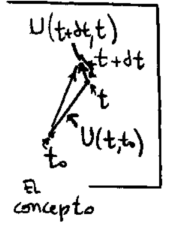
\includegraphics[width=0.3\textwidth]{images/teo2_5.pdf}	 
	\end{center}
	\caption{}
\end{figure} 



% =================================================================================================
\section{Dinámica cuántica}
% =================================================================================================

\subsection{Casos de solución de $U(t,t_o)$}

\begin{itemize}
 \item Supongamos $ H \neq H(t)$, entonces
 \[
	U( t, t_0) = \euler^{-i/\hbar H (t-t_0)} 
 \]
 \item Sea $ H = H(t)$, entonces
 \[
	U( t, t_0) = \euler^{-i/\hbar \int_{t_0}^t H(t')dt'} 
 \]
 y la integral puede hacerse una vez conocida la expresión de $H(t)$.
 \item Sea $ H = H(t)$ con $[H(t_1),H(t_2)] \neq 0$ entonces
 \begin{multline*}
	U( t, t_0) =  1 + \sum_{n=1}^{\infty} \left( \frac{-i}{\hbar}\right)^n 
		\int_{t_0}^t dt_1 \int_{t_0}^{t_1} dt_2 \int_{t_0}^{t_2} dt_3 ... \times \\
			\int_{t_0}^{t_{n-1}} dt_n H(t_1) H(t_2) ... H(t_n)    
 \end{multline*}
%  \[
% 	U( t, t_0) =  1 + \sum_{n=1}^{\infty} \left( \frac{-i}{\hbar}\right)^n 
% 		\int_{t_0}^t dt_1 \int_{t_0}^{t_1} dt_2 \int_{t_0}^{t_2} dt_3 ... \int_{t_0}^{t_{n-1}} dt_n 
% 			H(t_1) H(t_2) ... H(t_n)  
%  \]
 y esta es la serie de Dyson (del físico Freeman Dyson().)
\end{itemize}

El problema que suscita es debido a que si $H$ a diferentes tiempos no conmuta no podemos poner la exponencial en serie 
de potencias. En realidad $\exp({\square})$ tiene sentido sólo si la serie 
\[
	\sum_{n=0}^{\infty}  \frac{1}{n!}\square^n
\]
tiene sentido; es decir, si no surgen ambigüedades al tomar la potencia $n$-ésima del operador $\square$.
\notamargen{El operador $\square$ no se deja poner sombreros, quiere andar con la cabeza descubierta}

Para el caso 1 es simplemente 
 \[
	a
 \]
pero para el caso 3 es 
 \[
	a
 \]
puesto que al operar es 
\[
	a
\]
pues $[H(t'),H(t'')]\neq 0$. En el caso 2 $(\int_{t_0}^t H(t')dt' )^n$ no tiene problemas puesto que está provista la 
conmutatividad.

\subsection{Soluciones útiles}

Primeramente conseguimos un $\hat{A}$ tal que $[ A, H ]=0$ y entonces (estoy considerando $ H \neq H(t)$ )
\[
	a,
\]
luego 
\[
	a
\]
con $\hat{H}$ y $\hat{A}$ conmutan se tiene
\[
	a
\]

Entonces operamos con el $H$ para 
\[
	a
\]
y así 
\[
	a
\]
de manera que comparando con 
\[
	a
\]
El coeficiente es el mismo pero le hemos sumado una fase $\exp(-iE_{a'}(t-t_0)/\hbar)$ que no es global.

\subsection{Evolución de valores de expectación}

Recordemos primeramente que los autoestados no evolucionan. Luego 
\[
	a
\]

La fase es global es considerar una autoestado. La podemos descartar (setear igual a uno)
\[
	a
\]

El valor de expectacion de un operador respecto a un autoestado no varía.
\[
	a
\]
\[
	a
\]
\[
	a
\]

El valor de expectación de un operador respecto a un estado general tiene una fase no global que produce términos de 
interferencia.

\subsection{Relaciones de conmutación}

\[
	[ A + B, C] = [A, C] + [B,C] 
\]
\[
	[A, B] = - [B,A]
\]
\[
	[A, B\cdot C] = B[A,C] +  [A,B]C
\]
\notamargen{Acá no es baca + caballo puesto que no conmutan.}
\[
	i\hbar[ A, B]_{\text{classic}} = [A, B]
\]
donde $[ , ]_{\text{classic}}$ es el corchete de Poisson.
Las relaciones de conmutación fundamentales son 
\[
	[x_i, x_j] = 0 \qquad [p_i, p_j]=0 \qquad [x_i,p_j] =i\hbar\delta_{ij}
\]
a las que podemos sumar
\[
	[x,f(p)] = i\hbar\dpar{f}{p} \qquad [p,G(x)] = i\hbar\dpar{G}{x} 
\]
\[
	[S_i,S_j] = i\hbar \varepsilon_{ijk}S_k
\]

\subsection{La ecuación de Schrödinger}

\[
	a \text{con} \qquad \hat{H} = \frac{\hat{p}^2}{2m} + V(\hat{x}) 
\]
Puedo meter un bra $\Bra{x'}$ que no depende del tiempo y entonces 
\[
	a
\]
\[
	a
\]
de manera que resulta la ecuación de Schrödinger
\[
	a .
\]

\subsection{Representación de Heisenberg}

Los kets y los operadores no tienen sentido físico, pero sí los valores de expectación : toda física podrá modificar 
los primeros pero debe conservar los valores de expectación. Así tenemos dos representaciones posibles:

\begin{center}
\begin{tabular}{|l|l|}
\hline
Schrödinger & Heisenberg \\
\hline
& \\
$\Ket{\alpha} \to U\Ket{\alpha} \quad $ & $\Ket{\alpha} \to \Ket{\alpha} \quad $ \\
& \\
$A \to A \quad $ & $A \to U^\dagger AU \quad$ \\
& \\
$\Ket{a'} \to \Ket{a'} \quad $ & $\Ket{a'} \to U^\dagger \Ket{a'} \quad $ \\
& \\
\hline
\end{tabular}
\end{center}
Así vemos que en Schrödinger los kets evolucionan y los operadores permanecen fijos; al igual que los autoestados.
En cambio en Heisenberg los kets no evolucionan pero sí lo hacen los operadores y los autoestados.

Deben notars que:
\begin{enumerate}
 \item Los productos internos no cambian con el tiempo
 \[
	a
 \]
 \item Los valores de expectacion son los mismos en ambos esquemas
 \[
	a
 \]
 \[
	\Braket{A}^{(S} = \Braket{A}^{(H} \qquad A(t)^H = U(t)^\dagger A^S U(t)
 \]
\end{enumerate}

El operador $\hat{A}$ en Schrödinger no depende explícitamente del tiempo. La idea es que le ``pegamos'' a los 
operadores la evolución temporal de los kets.
\[
	a
\]
pero a $t=t_0$ las representaciones coinciden,
\[
	a
\]

\subsubsection{La ecuación de Heisenberg}

\[
	a
\]
\[
	\Rightarrow 
\]
\[
	a
\]
\[
	a
\]
\[
	a
\]
y llegamos a la ecuación de Heisenberg
\[
	\dpar{A^{(H)}}{t} = \frac{1}{i\hbar} [ A^{(H)}, H^{(H)}]
\]
si $A^{(H)}$ conmuta con el $H^{(H)}$, entonces $A^{(H)}$ es una cantidad conservada (una constante de movimiento).
En ese caso el operador no depende del tiempo y entonces $A^{(H)} = A^{(S)}$.

\subsubsection{Evolución de autoestados}

\[
	a,
\]
aplico un $U^\dagger$ a ambos lados y entonces 
\[
	a
\]
los $a'$ no dependen de la representación porque tienen significado físico. Entonces los $\Ket{a'}$ evolucionan
\[
	a
\]
\[
	a
\]
\[
	a
\]
puesto que recordemos, nota importante,
\[
	a
\]
entonces $H$ es el mismo en ambas puesto que $\hat{U} =\hat{U}(\hat{H}) $ y $[U,H]=0$.

De esta forma los autoestados evolucionan al revés 
\[
	a
\]

Podemos ver de otro modo la equivalencia
\[
	a
\]
pero 
\[
	a
\]
\[
	a
\]

\subsubsection{Coeficientes}

Los coeficientes en Schrödinger y en Heisenberg son 
\[
	a
\]
Entonces en Schrödinger es 
\[
	a
\]
mientras que en Heisenberg es 
\[
	a
\]

Los coeficientes en las expresiones son iguales como corresponde a todo magnitud que tiene sentido físico, pues 
$|c_a(t)|^2$ es la probabilidad.

\subsection{Teorema de Ehrenfest}

Para una partícula libre, donde $p(t)=p(0)$ es constante de movimiento,
\[
	x^{(H)} = x(0) + \frac{p(0)}{m}t
\]
y se tiene 
\[
	[x(t),x(0)] = -\frac{i\hbar}{m}t
\]
\[
	H = \frac{p^2}{2m} + V(x)
\]
\[
	\dtot{P}{t} = \frac{1}{i\hbar}[p,H] = \frac{1}{i\hbar}[p,V(x)] = 
	\frac{1}{i\hbar}\left( -i\hbar\dpar{V}{x}\right),
\]
de modo que 
\[
	\dtot{P}{t} = -\dpar{V}{x} \qquad \longrightarrow \quad m \dtot[2]{x}{t} = -\dpar{V}{x} 
\]
\[
	p = m \dtot{x}{t} \qquad \dtot{p}{t} = m \dtot[2]{x}{t} 
\]
donde estamos usando 
\[
	\dpar{A^H}{t} = \frac{1}{i\hbar}[A^H,H]
\]

Es necesario remarcar que relaciones como $[x,p]=i\hbar$ son para operadores en la picture de Schrödinger, donde los 
operadores no cambian en el tiempo. Estamos en efecto haciendo $[x(0),p(0)]=i\hbar$
\[
	\Braket{\alpha,t_0|m \dtot[2]{x}{t}|\alpha,t_0} = - \Braket{\alpha,t_0|\dpar{V}{x}|\alpha,t_0}
\]
\[
	m\dpar[2]{}{t}\Braket{\alpha,t_0| x^H |\alpha,t_0} = -\Braket{\alpha,t_0|\dpar{V}{x}|\alpha,t_0}
\]
y entonces el teorema de Ehrenfest es 
\[
	m \dpar[2]{}{t} \Braket{x^{(s)}} = - \Braket{ \dpar{V^{(s)}}{x}}
\]
los valores de expectación son iguales en ambas representaciones.
% 
% =================================================================================================
\section{El oscilador armónico}
% =================================================================================================

Para el oscilador armónico 1D  el hamiltoniano y energía eran
\[
	H = \frac{p^2}{2m} + \frac{m\omega^2 x^2}{2} \qquad E = \hbar \omega \left( n + \frac{1}{2} \right)
\]
pero este problema puede resolverse usando un nuevo operador $\hat{a}$
\[
	\hat{a} = \sqrt{\frac{m\omega}{2\hbar}}\left( x + i\frac{p}{m\omega} \right) \qquad \text{con} \quad 
	\hat{a}^\dagger = \sqrt{\frac{m\omega}{2\hbar}}\left( x - i\frac{p}{m\omega} \right)
\]
que es suma de $\hat{x}, \hat{p}$ pero que no es hermítico. Cumple que 
\[
	[a , a^\dagger ] = 1 \qquad a a^\dagger =  \frac{H}{\hbar\omega} -1 \qquad 
	H = \hbar\omega \left( a a^\dagger + \frac{1}{2} \right),
\]
donde se define el operador número $\hat{N}\equiv a^\dagger a$ que al verificar $[\hat{N},\hat{H}]=0$ tienen base de 
autoestados en común $\{ \Ket{n} \}$. En efecto 
\[
	\hat{N} \Ket{n} = n\Ket{n} \qquad
	\hat{H} \Ket{n} = \hbar\omega \left( n + \frac{1}{2} \right) \Ket{n}
\]
siendo $n$ el número de cuantos de energía.
Se cumplen además 
\[
	[N,a] = [a^\dagger a,a] = - [ a, a^\dagger a ] = - \left( a^\dagger [a,a] + [a,a^\dagger]a \right) =
	-a
\]
\[
	[N,a^\dagger] = [a^\dagger a, a^\dagger ] = - [a^\dagger , a^\dagger a ] =
	- \left( a^\dagger [a^\dagger,a] + [a^\dagger,a]a^\dagger \right) = a^\dagger
\]

Queremos ver que le  hace $a^\dagger$  a un autoestado $\Ket{n}$ y luego $a$ sobre el mismo.
\[
	N a^\dagger \Ket{n} = ([N, a^\dagger] + a^\dagger N) \Ket{n} =
	a^\dagger \Ket{n} + a^\dagger n \Ket{n} 
\]
\[
	\Hat{N} (a^\dagger\Ket{n}) = (n+1)(a^\dagger\Ket{n})
\]
Entonces, como no hay degeneración y tenemos $N\Ket{n'} = n'\Ket{n'}$ entonces 
\[
	a^\dagger \Ket{n} = c_1 \Ket{n+1},
\]
y procediendo de modo idem para $a\ket{n}$ será
\[
	a \Ket{n} = c_2 \Ket{n-1}
\]
Luego,
\[
	a^\dagger \Ket{n} = c_1 \Ket{n+1} \overbrace{\longrightarrow}^{DC} 
	\Bra{n+1} c_1^* = \Bra{n} a 
\]
\[
	a \Ket{n} = c_2 \Ket{n-1} \overbrace{\longrightarrow}^{DC} \Bra{n-1} c_2^* = \Bra{n} a^\dagger
\]
y entonces 
\[
	\Braket{n|N|n} = n \Braket{n|n} = n =  \Braket{n| a^\dagger a |n} =  \Braket{n-1|c_2^* c_2|n-1} =
	|c_2|^2 \Braket{n-1|n-1}
\]
\[
	n = \Braket{n|aa^\dagger-1|n} = -1 + \Braket{n|aa^\dagger|n} = - 1 + \Braket{n+1|c_1^*c_1|n+1} =
	-1 + |c_1|^2 \Braket{n+1|n+1}
\]
siendo
\[
	|c_2| = \sqrt{n} \qquad |c_1| = \sqrt{n+1} 
\]
\[
	\hat{a}^\dagger \Ket{n} = \sqrt{n+1} \Ket{n+1} \qquad  \hat{a}\Ket{n} = \sqrt{n} \Ket{n-1} 
\]
y entonces de esta forma $\hat{a}^\dagger$ es el operador de creación de cuantos y $\hat{a}$ el de aniquilación.

\subsection{El estado fundamental $\Braket{0}$}

\[
	a \Ket{n}  \overbrace{\longrightarrow}^{DC} \Bra{n} a^\dagger
\]
y desde el postulado para productos internos,
\[
	(\Bra{n}a^\dagger)(a\Ket{n}) \geq 0 \quad n \Braket{n|n} \geq 0 \Rightarrow n \geq 0 
\]
entonces $n$ cabalga por los naturales.
Si hacemos 
\[
	a\Ket{n} = \sqrt{n} \Ket{n-1}, \qquad  a^2 \Ket{n} = \sqrt{n}\sqrt{n-1} \Ket{n-2} \; ...
\]
en algún momento se llega a $\Ket{n=0}$, entonces $E_0 = \hbar\omega/2$ y 
\[
	\Ket{0} \equiv \text{El fundamental}
\]
y no se puede bajar más,
\[
	\hat{a}\Ket{0} = 0.
\]

Por otra parte, con el $\hat{a}^\dagger$ se puede llegar a cualquier estado
\[
	a^\dagger \Ket{0} = \sqrt{1} \Ket{1}, \qquad  a^{\dagger 2} \Ket{0} = \sqrt{1}\sqrt{2} \Ket{2} = 
	\sqrt{1}\sqrt{2}\sqrt{3} \Ket{3}
\]
\[
	\frac{{(a^{\dagger})}^n}{\sqrt{n}!} \Ket{0} = \Ket{n}
\]

Las matrices de $\hat{a},\hat{a}^\dagger$ sólo tienen una diagonal corrida de elementoss 
\[
	\Braket{n'|a|n} = \sqrt{n} \Braket{n'|n-1} = \sqrt{n} \delta_{n',n-1}
\]
\[
	\Braket{n'|a^\dagger|n} =  \sqrt{n-1} \Braket{n'|n+1} = \sqrt{n-1} \delta_{n',n+1}
\]

También puede verse que 
\[
	\Braket{n|x|n}= 0 \qquad \Braket{n|p|n}= 0
\]
y por ello 
\[
	\Braket{(\Delta x)^2}_{\Ket{0}} \Braket{(\Delta p)^2}_{\Ket{0}} = \frac{\hbar^2}{4} 
\]
el estado fundamental es el de incerteza mínima.

\subsection{Función de onda}

Siendo $\Psi_n(x') = \Braket{x'|n}$ quiero evaluar $\Psi_0(x') = \Braket{x'|0}$ y ver que como 
\[
	\Braket{x'|a|0}= 0 
\]
tengo 
\[
	0 = \sqrt{ \frac{m\omega}{2\hbar} } \Braket{x'|x+\frac{ip}{m\omega}|0} =
	\sqrt{ \frac{m\omega}{2\hbar} } \left[ x'\Braket{x'|0} + \frac{i}{m\omega}\Braket{x'|p|0} \right]
\]
\[
	x' \Braket{x'|0} + \frac{i}{m\omega} (-i\hbar) \dpar{}{x} \Braket{x'|0} = 0
\]
entonces 
\[
	x' \Braket{x'|0} = - \frac{\hbar}{m\omega} \dpar{}{x'}\Braket{x'|0} 
\]
\[
	- \int \frac{m\omega}{\hbar} x' dx' = \int \frac{d \Braket{x'|0}}{\Braket{x'|0}} \Rightarrow 
	\Braket{x'|0} = \kappa \euler^{-m\omega x^{'2}/(2\hbar)}
\]
y entonces 
\[
	1 = \int_{-\infty}^{\infty} \Braket{0|x'}\Braket{x'|0} dx' = 
	\int_{-\infty}^{\infty} |\kappa|^2 \euler^{-m\omega x^{'2}/\hbar} dx' =
	|\kappa|^2 \sqrt{\frac{\pi\hbar}{m\omega}} 
\]
\[
	|\kappa| = \left( \frac{m\omega}{\pi\hbar} \right)^{1/2} = \frac{1}{(\pi x_0^2)^{1/4}}
\]
donde usamos el conocido resultado $\int_{-\infty}^\infty \exp( - a x^2) dx = \sqrt{\pi/a}$, llegamos al llamado pack 
gaussiano.
\[
	\Braket{x'|0} = \frac{1}{(\pi x_0^2)^{1/4}} \euler^{-\frac{1}{2}\left( x'/x_0 \right)^2}
\]
El estado fundamental tiene incerteza mínima y debe corresponder a un paquete gaussiano.

Notemos que $\hat{a}^\dagger$ crea sobre ket y aniquila sobre bra, mientras que $\hat{a}$ aniquila sobre ket y crea 
sobre bra,
\[
	a^\dagger \Ket{n} = \sqrt{n+1} \Ket{n+1} \Rightarrow \Bra{n} a = \Bra{n+1} \sqrt{n+1}
\]
\[
	a \Ket{n} = \sqrt{n} \Ket{n-1} \Rightarrow \Bra{n} a^\dagger = \Bra{n-1} \sqrt{n}
\]

\subsection{Interferencia en experimento de Young}

Consideremos la situación depicted en la figura bajo estas líneas

\begin{figure}[htb]
	\begin{center}
	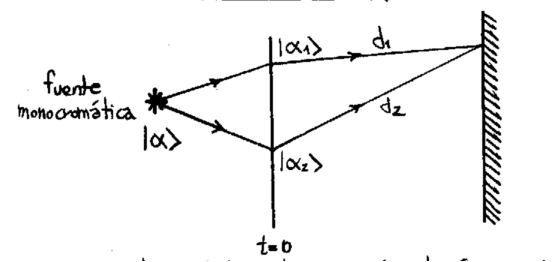
\includegraphics[width=0.6\textwidth]{images/teo2_6.pdf}	 
	\end{center}
	\caption{}
\end{figure} 

Uso $\hat{H}$ de partículas libres.
\[
	\frac{1}{2} \Ket{\alpha} = \Ket{\alpha_1} = \Ket{\alpha_2}
\]
para $t>0$ se tiene 
\[
	\Ket{\tilde{\alpha_1}} = \euler^{ -i H t /\hbar } \Ket{\alpha_1} =
		\euler^{ -i E_\alpha t /\hbar } \Ket{\alpha_1}	
\]
\[
	\Ket{\tilde{\alpha_2}} = \euler^{ -i E_\alpha t /\hbar } \Ket{\alpha_2}	
\]

En la pantalla debe verse la interferencia de los dos estados solapados.
\[
	\Ket{\tilde{\alpha}} = \Ket{\tilde{\alpha_1}} + \Ket{\tilde{\alpha_2}} =
		\euler^{ -i E_\alpha \frac{d_1}{v} /\hbar } \Ket{\alpha_1} +
		\euler^{ -i E_\alpha \frac{d_2}{v} /\hbar } \Ket{\alpha_2}	
\]
\[
	\Ket{\tilde{\alpha}} = \frac{1}{2} \euler^{ -i E_\alpha \frac{d_1}{v} /\hbar } 
		| 1 + \euler^{ -i E_\alpha \frac{d_2-d_1}{v} /\hbar } | \Ket{\alpha_1}
\]
y si definimos
\[
	\beta=E_\alpha \frac{d_2-d_1}{v} /\hbar,
\]
resulta entonces
\[
	\Braket{\tilde{\alpha}|\tilde{\alpha}} = \frac{1}{4}| 1 +  \euler^{ -i E_\alpha \frac{d_2-d_1}{v} /\hbar } |^2 =
		\frac{1}{4}( (1+\cos\beta)^2 + \sin^2\beta ) =
			\frac{1}{2} + \frac{1}{2}\cos\left( \beta \right).
\]


Al partir el estado $\Ket{\alpha_1} $ y volver a unirlo en $\Ket{\alpha_1} + \Ket{\alpha_2}$ vemos una intensidad que 
dependa de la diferencia de camino.

\subsection{Cambio de cero del potencial}

En mecánica clásica la física de un problema no se ve afectada por un cambio de gauge.
Si movemos el cero de potencial, la situación física es la misma.
Veamos qué sucede en mecánica cuántica.
\[
	\Ket{\alpha,t,t_0} = \euler^{ -i (p^2/2m + V(x))(t-t_0)/\hbar} \Ket{\alpha,t_0}
\]
\[
	\Ket{\tilde{\alpha},t,t_0} = \euler^{ -i (p^2/2m + V(x) + V_0)(t-t_0)/\hbar} \Ket{\alpha,t_0}
\]
\[
	\Ket{\tilde{\alpha},t,t_0} = \euler^{ -i V_0(t-t_0)/2 }\Ket{\alpha,t,t_0}
\]
y entonces vemos que $\Ket{\tilde{\alpha},t}$ y $\Ket{\alpha,t}$ difieren en una fase, de manera que los valores de 
expectación no cambian (con $V_0$ constante).

\begin{figure}[htb]
	\begin{center}
	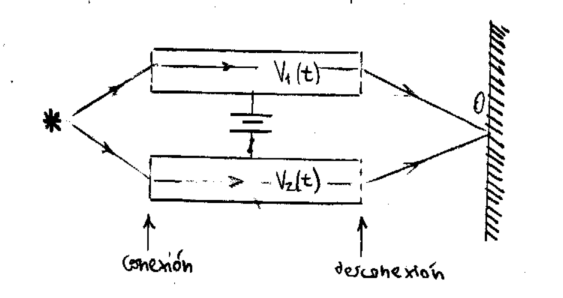
\includegraphics[width=0.6\textwidth]{images/teo2_7.pdf}	 
	\end{center}
	\caption{}
\end{figure} 

Este es un experimento ideal (pensado). Dentro de los cilindros hay campo nulo. Se varia el $V$ abriendo y cerrando la 
llave a la entrada y a la salida.
Se cambia la fase de las partículas inferiores respecto de las superiores, entonces habrá interferencia en $O$.

Clásicamente no hay variación,
\[
	\Delta \text{fase} = -\frac{i}{\hbar}\euler \int _{t_1}^{t_2} V_1(t) - V_2(t) dt = 
	-\frac{i}{\hbar}\euler \Delta V
\]

Lo que realmente cuenta es la diferencia de potencial $\Delta V$, la cual sí tiene sentido físico porque es 
independiente de la medida y porque pueden escribirse los campos en función de aquella.
\[
	E = - \Nabla\phi - \frac{1}{c}\dpar{\vb{A}}{t}
\]
\[
	H = \frac{1}{2m} \left( \vb{p} - \frac{\euler\vb{A}}{c}\right)^2 + \euler\phi 
\]
\[
	\dtot{H}{t} = \frac{1}{i\hbar}[x_i,H] = \frac{p_i  \euler A_i}{m}
\]

% =================================================================================================
\section{El propagador}
% =================================================================================================

Físicamente representa la proababilidad de transición entre autoestados por el paso del tiempo,
$ \Ket{x'}_{t_0} \longrightarrow \Ket{x''}_t$
\[
	a
\]
\[
	b
\]
\[
	c
\]

Podemos pensar que el propagador lleva la función de onda desde $t_0$ a $t$. Se puede escribir:
\[
	a
\]
y metemos un observable $\hat{A}$ donde $[A,H]=0$ y $A\Ket{a'}=a\Ket{a'}$.

El propagador depende del potencial, pero no de la función de onda inicial. Se debe cumplir que:
\[
	b
\]
\[
	c
\]
\[
	d
\]
y entonces el propagador es una función de Green que satisface 
\[
	d
\]
con $K(x'',t;x',t_0)=0 $ si $t<0$ que es la condición de contorno.

\subsection{El propagador de la partícula libre}

\[
	a
\]
\[
	a
\]
\[
	b
\]

También se puede escribir el propagador en la representación de Heisenberg,
\[
	a
\]
\[
	K(x'',t;x',t_0) = \Braket{x'',t | x',t_0}.
\]

El propagador cumple con la propiedad de composición (como el $U(t,t_0)$), es decir:
\[
	a
\]

\section{Integrales de camino de Feynmann}

Consideramos una partícula yendo de $(x_1,t_1)$ a $(x_N,t_N)$. Dividimos el tiempo 
\[
	a
\]
y queremos ver la amplitud de transición desde el estado 1 al $N$.

\[
	a
\]

Se puede pensar como que estamos sumando sobre todos los posibles caminos entre $(x_1,t_1)$ y $(x_N,t_N)$ 
fijos. En mecánica clásica teníamos un solo camino, el que minimizaba la acción $S$
\[
	\delta \int_{t_1}^{t_2} \Lag dt = \delta S = 0
\]
pero en cambio en mecánica cuántica todos los caminos aportan. En un libro de Dirac, Feymann lee 
\[
	a
\]
Definiremos
\[
	\equiv 
\]
Luego para considerar la suma sobre todos los segmentillos a lo largo de un camino tendremos
\[
	\prod_{n=2}^N \euler^{i/\hbar S(n,n-1)} =
\]
y hay que considerar TODOS los posibles caminos 
\[
	\propto \sum_{caminos} \euler^{i/\hbar S(N,1)} 
\]
cuando $\hbar \to 0$ las trayectorias contribuyen con una cantidad que oscila loca y violentamente. Tienden a 
la cancelación para caminos aledaños. Por el $\hbar \sim 0$ la fase es grande y entonces se cancelan.
Esto no ocurre cerca del camino (real) que cumple 
\[
	\delta S(N,1) = 0
\]
Para trayectorias cercanas la $\Delta fase$ no es grande y hay interferencia constructiva.
Para un $\delta t$ infinitesimal es 
\[
	a
\]
\[
	b
\]

Consideremos, por ejemplo, una partícula libre, entonces $V=0$ de modo que resolviendo 
\[
	a
\]
Esto no es otra cosa que el propagador de una partícula libre. Para un $\Delta t$ finito será 
\[
	+
\]
\[
	=
\]
siendo esta última la integral de camino de Feynmann.

En base a éstas Feynamn desarrolla una formulación equivalente de la mecánica cuántica que utiliza los 
conceptos de:
\begin{enumerate}
 \item Superposición
 \item Composición de la transición
 \item Límite clásico con $\hbar \to 0$
\end{enumerate}

Estas integrales contienen toda la información del sistema cuántico, aunque no sea sencillo extraerla.

Consideremos un propagador de $(x',0) \to (x',t)$
\[
	G(t) =
\]
\[
	G(t) =
\]
y tomando Laplace-Fourier 
\[
	\tilde{G}(t)
\]

La expresión 
\[
	\equiv Integral de camino de Feynmann
\]


















% %  	I d\vb{\ell} \times \vb{B} = \vb{J}  \cdot d\vb{S} d\vb{\ell}  \times \vb{B} =
% %   	\cos(\theta) dS \vb{J} d\ell \times \vb{B} = \\
% % 	\vb{J} \times \vb{B}  \cos(\theta) dS d\ell  = \vb{J} \times \vb{B}  d\vb{S} \cdot d\vb{\ell}  = 
% % 	\vb{J} \times \vb{B}  dV 
% % \end{align*}
% \[
%   	I d\vb{\ell} \times \vb{B} = \vb{J}  \cdot d\vb{S} d\vb{\ell}  \times \vb{B} =
%   	\cos(\theta) dS \vb{J} d\ell \times \vb{B} = 
% \]
% \[
% 	\vb{J} \times \vb{B}  \cos(\theta) dS d\ell  = \vb{J} \times \vb{B}  d\vb{S} \cdot d\vb{\ell}  = 
% 	\vb{J} \times \vb{B}  dV 
% \]
% 
% \subsection{Fuerza de un circuito sobre otro}
% 
% La fuerza de un circuito 2 sobre otro circuito 1 puede calcularse con un poco de paciencia como sigue
% \[
% 	F_{12} = \frac{1}{c} \int_{\Gamma_1} I_1 d\vb{\ell}_1 \times \left\{
% 	\frac{1}{c} \int_{\Gamma_2} \frac{I_2 d\vb{\ell}_2 \times (\vb{x}_1 - \vb{x}_2)}{|\vb{x}_1 - \vb{x}_2|^3} 
% 	\right\}
% \]
% \[
% 	F_{12} = \frac{I_1 I_2}{c^2} \int_{\Gamma_1} \int_{\Gamma_2} d\vb{\ell}_1 \times \left\{
% 	\frac{d\vb{\ell}_2 \times (\vb{x}_1 - \vb{x}_2)}{|\vb{x}_1 - \vb{x}_2|^3} 
% 	\right\}
% \]
% \[
% 	F_{12} = \frac{I_1 I_2}{c^2} \int_{\Gamma_1} \int_{\Gamma_2} d\vb{\ell}_2  \left\{
% 	\frac{d\vb{\ell}_1 \cdot (\vb{x}_1 - \vb{x}_2)}{|\vb{x}_1 - \vb{x}_2|^3} 
% 	\right\} - \int_{\Gamma_1} \int_{\Gamma_2} \frac{ (\vb{x}_1 - \vb{x}_2)}{|\vb{x}_1 - \vb{x}_2|^3} 
% 	\left\{ d\vb{\ell}_1 \cdot d\vb{\ell}_2 \right\}
% \]
% donde el primer término se comprueba nulo si se reescribe utilizando que
% \[
% 	\frac{ (\vb{x}_1 - \vb{x}_2)}{|\vb{x}_1 - \vb{x}_2|^3} = 
% 	\nabla_{\vb{x}_2} \frac{ 1 }{|\vb{x}_1 - \vb{x}_2|} =
% 	- \nabla_{\vb{x}_1} \frac{ 1 }{|\vb{x}_1 - \vb{x}_2|} 
% \]
% de manera que entonces
% \[
% 	- \int_{\Gamma_2} d\vb{\ell}_2  \int_{\Gamma_1} d\vb{\ell}_1 \cdot \nabla_{\vb{x}_1} \frac{ 1 }{|\vb{x}_1 - \vb{x}_2|} 
% \]
% donde se ve que es nula la última integral dado que 
% \[
% 	\int_{\Gamma_1} d\vb{\ell}_1 \cdot \nabla_{\vb{x}_1} = 0.
% \]
% 
% Entonces, se tiene 
% \[
% 	F_{12} = - \frac{I_1 I_2}{c^2} \int_{\Gamma_1} \int_{\Gamma_2} \frac{ (\vb{x}_1 - \vb{x}_2)}{|\vb{x}_1 - \vb{x}_2|^3} 
% 	\left( d\vb{\ell}_1 \cdot d\vb{\ell}_2 \right)
% \]
% que vale lo mismo si intercambiamos $\Gamma_1$ con $\Gamma_2$ en la integración. Podemos decir que con corrientes estacionarias
% vale el principio de acción y reacción: las fuerzas son iguales y de sentido opuesto.
% 
% 
% % =================================================================================================
% \section{Teorema de Helmholtz}
% % =================================================================================================
% 
% Nos dice que un campo vectorial está completamente determinado por su divergencia y su rotor.
% Por ejemplo, para un campo eléctrico 
% \[
% 	\vb{E} = \int_{V'} \rho \frac{\vb{x} - \vb{x}'}{|\vb{x} - \vb{x}'|^3} dV' = 
% 		- \int_{V'} \rho \nabla_{\vb{x}} \frac{ 1 }{|\vb{x} - \vb{x}'|} dV' = 
% 		- \nabla_{\vb{x}} \int_{V'}   \frac{ \rho }{|\vb{x} - \vb{x}'|} dV' = 
% \]
% y esta última es la integral de Poisson
% \[
% 	\vb{E} = - \nabla_{\vb{x}} \phi (\vb{x}).
% \]
% Entonces $\vb{E}$ es un gradiente y por ello 
% \[
% 	\nabla  \times \vb{E} = 0
% \]
% de manera que $\vb{E}$ es conservativo, cumple $\int \vb{E}\cdot d\vb{\ell} = 0$ o lo que
% es lo mismo, $\vb{E}$ es irrotacional.
% Hemos hecho la construcción de un potencial electrostático.
% 
% % =================================================================================================
% \section{Ley de Gauss}
% % =================================================================================================
% 
% 
% 
% \begin{figure}[htb]
% 	\begin{center}
% 	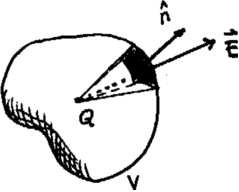
\includegraphics[width=0.35\textwidth]{images/fig_ft1_gauss.pdf}	 
% 	\end{center}
% 	\caption{}
% \end{figure} 
% \[
% 	\vb{E} \cdot \hat{n} = q \frac{\cos(\theta)}{r^2}
% \]
% y el ángulo sólido es
% \[
% 	\vb{E} \cdot \hat{n} dS = q \frac{\cos(\theta)}{r^2} dS
% \]
% \[
% 	\vb{E} \cdot \hat{n} dS = q d\Omega \qquad \longrightarrow \qquad 
% 	\int_{S\equiv\partial V} \vb{E} \cdot \hat{n} \; dS = q \int_S d\Omega =
% 	\begin{cases}
% 	 0 \quad \textrm{carga exterior}\\
% 	 4\pi \quad \textrm{carga interior}
% 	\end{cases}
% \]
% \[
% 	\int_S \vb{E} \cdot \hat{n} \; dS = 4\pi \sum_i q_i
% \]
% La ley de Gauss es
% \[
% 	\int_S \vb{E} \cdot \hat{n} \; dS = 4\pi Q_n
% \]
% donde $Q_n$ es la carga neta dentro de la superficie $S$. Al continuo pasa como 
% \[
% 	\int_S \vb{E} \cdot \hat{n} \; dS = 4\pi \int_V \rho \: dV
% \]
% de manera que 
% \[
% 	\int_V \divem{E} \; dV = \int_V 4\pi \rho \: dV
% \]
% y entonces
% \[
% 	\divem{E} = 4\pi \rho.
% \]
% 
% Por otro lado si \vb{E} es el gradiente de un potencial $\phi$ se tiene
% \[
% 	\divem{E} = \Nabla\cdot{(-\Nabla\phi)} = - \lapm\phi = 4\pi \rho
% \]
% y se desprenden las ecuaciones de Poisson,
% \[
% 	\lapm\phi = -4\pi \rho
% \]
% y de Laplace
% \[
% 	\lapm\phi = 0
% \]
% que es el caso particular de la anterior con cargas nulas.
% 
% La solución de la ecuación no homogénea es suma de una solución del homogéneo más una solución
% particular. La carga está relacionada a la solución particular.
% 
% \subsection{Gauges}
% 
% Dado que $\divem{B}=0$ entonces existe un \vb{A} tal que 
% \[
% 	\rotorm{A} = \vb{B}
% \]
% pero para caracterizar totalmente el \vb{A} tengo la libertad de definir a conveniencia
% \[
% 	\divem{A} \equiv \; \textrm{``el gauge''}.
% \]
% Casos particulares importantes son el gauge de Coulomb,
% \[
% 	\divem{A} = 0
% \]
% de manera que como 
% \[
% 	\Nabla \times (\rotorm{A}) = \Nabla(\divem{A}) - \lapm{\vb{A}} = \frac{4\pi}{c}\vb{J}
% \]
% se llega para el potencial electromagnético, bajo el gauge de Coulomb, a que 
% \[
% 	\lapm{\vb{A}} = - \frac{4\pi}{c}\vb{J} 
% \]
% 
% 	\begin{table}[hbt]
% 	\centering
%         \begin{tabular}{|c|c|}
% 		\hline
% 		& \\
% 		$\displaystyle{\vb{E} = \int_{V'} \frac{\rho(\vb{x}')(\vb{x}-\vb{x}')}{|\vb{x}-\vb{x}'|^3} dV' 
% 		}$ & $\displaystyle{\vb{B} = \frac{1}{c} \int_{V'} \frac{\vb{J}(\vb{x}') \times 
% 		(\vb{x}-\vb{x}')}{|\vb{x}-\vb{x}'|^3} dV'}$ \\
% 		& \\
% 		\hline
% 		Ley de Gauss & Ley de Ampere \\
% 		& \\
% 		$\displaystyle{\int_S \vb{E}\cdot d\vb{S} = 4\pi Q_n}$ &
% 		$\displaystyle{\int_\Gamma \vb{B}\cdot d\vb{\ell} = \frac{4\pi}{c} I_c}$ \\
% 		& \\
% 		\hline
% 		&\\
% 		$\divem{E} = 4\pi\rho$ & $\divem{B} = 0$ \\
% 		$\rotorm{E} = 0$ & $\rotorm{B} = \frac{4\pi}{c}\vb{J}$ \\
% 		& \\
% 		\hline
% 		& \\
% 		$\vb{E} = - \Nabla\phi$ & $\vb{B} = \rotorm{A}$ \\
% 		& \\
% 		\hline
%         \end{tabular} 
% 	\caption{}
% 	\end{table} 
% 
% La operación de tomar rotor y el producto vecrtorial cambian el carácter de los vectores: de
% polares pasan a axiales y viceversa.
% 
% La fuerza general sobre una distribución de carga es
% \[
% 	\vb{F} = \int_{V'} \rho \vb{E} dV' + \frac{1}{c} \int_{V'} \vb{J} \times \vb{B} dV'. 
% \]
% 
% \subsection{Delta de Dirac}
% 
% Una densidad de carga puntual se puede escribir mediante una delta de Dirac de acuerdo a
% \[
% 	\rho(\vb{x}') = q\: \delta (\vb{x} - \vb{x}') = \begin{cases}
% 	                                               0 \qquad \vb{x} \neq \vb{x}' \\
% 	                                               \infty \qquad \vb{x} = \vb{x}'\\
% 	                                              \end{cases}
% \]
% siendo las dimensiones de la delta las de $1/L^3$ y cumpliéndose 
% \[
% 	\int_{V'} \delta (\vb{x} - \vb{x}') dV' = 1
% \]
% \[
% 	\delta (\vb{x} - \vb{x}') = \frac{1}{h_1h_2h_3} \delta(q_1-q_1') \delta(q_2-q_2') \delta(q_3-q_3')
% \]
% donde $q_1, q_2$ y $q_3$ son coordenadas curvilíneas generales y $h_1h_2h_3$ es el jacobiano
% de la transformación.
% Luego
% \[
% 	\int f(\vb{x}) \delta' (\vb{x} - \vb{x}_0) dx = -f'(\vb{x}_0)
% \]
% 
% 
% 
% \subsection{reflexión}
% 
% Un vector polar sufre reflexión especular mientras que un vector axial ({\it pseudovector})
% sufre una antireflexión especular. Ver la figura.
% 
% \begin{figure}[htb]
% 	\begin{center}
% 	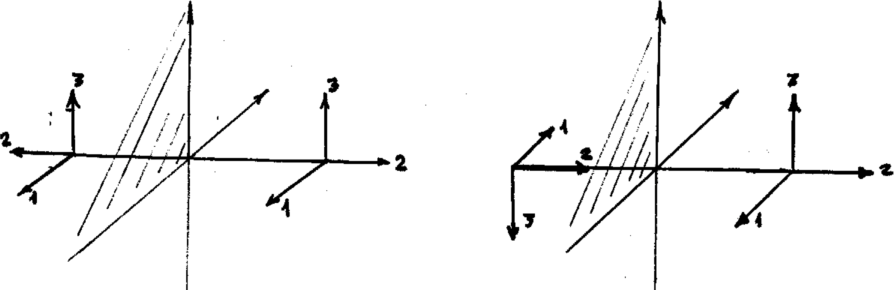
\includegraphics[width=0.6\textwidth]{images/fig_ft1_reflexvect.pdf}	 
% 	\end{center}
% 	\caption{}
% \end{figure} 
% 
% Una reflexión más una rotación permite eliminar componentes de campo.
% Una simetría más una rotación-traslación permite eliminar dependencias.
% 
% Lo primero que debe hacerse es escribir bien la \vb{J} a partir del dato de la corriente
% (que es el que se suele tener) mediante
% \[
% 	i = \int_S \vb{J} \cdot d \vb{S}
% \]
% En cambio, para \vb{A} es más fácil usar
% \[
% 	\vb{B} = \rotorm{A}
% \]
% y despejar de aquí la ecuación diferencial que emplear
% \[
% 	\vb{A} = \frac{1}{c} \int_V \frac{\vb{J}}{|\vb{x}-\vb{x}'|} dV
% \]
% 
% 
% \section{El potencial vector}
% 
% Por la ley de Biot y Savart,
% \[
% 	\vb{B} = \frac{1}{c} \int_{V'} \frac{\vb{J}(\vb{x}') \times (\vb{x}-\vb{x}')}{|\vb{x}-\vb{x}'|^3} 
% 	dV' = \Nabla_x \times \frac{1}{c} \int_{V'} \frac{\vb{J}(\vb{x}')}{|\vb{x}-\vb{x}'|} dV'
% \]
% de modo que
% \be
% 	\vb{A} = \frac{1}{c} \int_{V'} \frac{\vb{J}(\vb{x}')}{|\vb{x}-\vb{x}'|} dV'
% 	\label{potvec}
% \ee
% pero 
% \[
% 	\vb{A}' \equiv \vb{A} + \Nabla \Psi
% \]
% es tan buen potencial vector como \vb{A} puesto que los rotores verifican $\rotorm{A}=\rotorm{A}'=\vb{B}$,
% de lo cual extraemos en conclusión que el potencial vector está definido a menos del gradiente de una
% función escalar.
% 
% Tomándole el rotor a \eqref{potvec} y considerando $\Nabla'\cdot\vb{J}(\vb{x}')=0$ lo cual se verifica si
% la corriente es estacionaria se tiene 
% \[
% 	\rotorm{B} = \frac{4\pi}{c} \vb{J}(\vb{x})
% \]
% y entonces
% \[
% 	\int_S \rotorm{B} \cdot d\vb{S} = \frac{4\pi}{c} \int_S \vb{J}(\vb{x}) \cdot d\vb{S}
% \]
% y por el teorema de Stokes arribamos a
% \[
% 	\int_{\Gamma\equiv\partial S} \vb{B}\cdot d\vb{\ell} = \frac{4\pi}{c} I_\Gamma
% \]
% que es la ley de Ampere. Notemos que $I_\Gamma$ es la corriente concatenada por el lazo $\Gamma$.
% Además
% \[
% 	\rotorm{B} = \Nabla\times(\rotorm{A}) = \Nabla(\divem{A}) - \nabla^2 \vb{A} = \frac{4\pi}{c}\vb{J}
% \]
% pero utilizando el gauge de Coulomb es $\divem{A}=0$ y entonces
% \[
% 	\nabla^2 \vb{A} = -\frac{4\pi}{c}\vb{J}
% \]
% que es una ecuación de Poisson vectorial.
% 
% Magnetostática y electrostáctica son gobernadas por ecuaciones de Poisson para potenciales $\vb{A},\phi$ y
% el problema entonces se reduce a resolverlas para luego hallar los campos por derivación.
% 
% \section{Unicidad de problemas de potencial}
% 
% Si dos problemas satisfacen iguales condiciones de contorno entonces en el recinto encerrado por
% ese contorno tienen igual solución.
% 
% Si en un recinto $R$
% \be
% 	\phi_1|_{cont} = \phi_2|_{cont}
% 	\label{potnounico}
% \ee
% pero se da para el interior de $R$ que $\phi_1\neq\phi_2$ entonces se tiene sucesivamente
% \[
% 	U \equiv \phi_1 - \phi_2 \qquad \qquad \Nabla U = \Nabla \phi_1 - \Nabla \phi_2
% \]
% \[
% 	\lapm{U} = \lapm{\phi_1} - \lapm{\phi_2} = -4\pi \rho + 4\pi\rho = 0
% \]
% \[
% 	\Nabla\cdot\left( U\Nabla U \right) = U\left( \Nabla\cdot\Nabla U \right) + \Nabla U \cdot \Nabla U
% \]
% \[
% 	\int_V \Nabla\cdot\left( U\Nabla U \right) dV = \int_V U \lapm{U}  + (\lapm{U})^2 dV =  \int_V (\lapm{U})^2 dV
% \]
% llegando al último miembro porque el potencial $U$ cumple la ecuación de Laplace. Luego,
% \[
% 	\int_V (\lapm{U})^2 dV = \int_S U\Nabla{U} \cdot d\vb{S} = 0
% \]
% habiéndose pasado a la integral de superficie por el teorema de la divergencia y anulando el valor global porque 
% $U$ en el contorno es nula (recuérdese \eqref{potnounico}). Además, 
% \[
% 	\Nabla{U} \cdot d\vb{S}  \longrightarrow \left.\dpar{U}{\hat{n}}\right|_{cont}
% \]
% luego,
% \[
% 	\Nabla U = 0 \qquad \Nabla\phi_1 = \Nabla\phi_2 
% \]
% y entonces
% \[
% 	\phi_1 = \phi_2 .
% \]
% a menos, por supuesto, de una constante.



% \bibliographystyle{CBFT-apa-good}	% (uses file "apa-good.bst")
% \bibliography{CBFT.Referencias} % La base de datos bibliográfica

\end{document}

	
% 		\documentclass[10pt,oneside]{CBFT_book}
	% Algunos paquetes
	\usepackage{amssymb}
	\usepackage{amsmath}
	\usepackage{graphicx}
	\usepackage{libertine}
	\usepackage[bold-style=TeX]{unicode-math}
	\usepackage{lipsum}

	\usepackage{natbib}
	\setcitestyle{square}

	\usepackage{polyglossia}
	\setdefaultlanguage{spanish}
	



	\usepackage{CBFT.estilo} % Cargo la hoja de estilo

	% Tipografías
	% \setromanfont[Mapping=tex-text]{Linux Libertine O}
	% \setsansfont[Mapping=tex-text]{DejaVu Sans}
	% \setmonofont[Mapping=tex-text]{DejaVu Sans Mono}

	%===================================================================
	%	DOCUMENTO PROPIAMENTE DICHO
	%===================================================================

\begin{document}

% =================================================================================================
\chapter{Formalismo matemático}
% =================================================================================================

Kets y todo eso





% \bibliographystyle{CBFT-apa-good}	% (uses file "apa-good.bst")
% \bibliography{CBFT.Referencias} % La base de datos bibliográfica

\end{document}

	
		\documentclass[10pt,oneside]{CBFT_book}
	% Algunos paquetes
	\usepackage{amssymb}
	\usepackage{amsmath}
	\usepackage{graphicx}
	\usepackage{libertine}
	\usepackage[bold-style=TeX]{unicode-math}
	\usepackage{lipsum}

	\usepackage{natbib}
	\setcitestyle{square}

	\usepackage{polyglossia}
	\setdefaultlanguage{spanish}
	



	\usepackage{CBFT.estilo} % Cargo la hoja de estilo

	% Tipografías
	% \setromanfont[Mapping=tex-text]{Linux Libertine O}
	% \setsansfont[Mapping=tex-text]{DejaVu Sans}
	% \setmonofont[Mapping=tex-text]{DejaVu Sans Mono}

	%===================================================================
	%	DOCUMENTO PROPIAMENTE DICHO
	%===================================================================

\begin{document}

% 
% =================================================================================================
\chapter{El oscilador armónico}
% =================================================================================================

Para el oscilador armónico 1D  el hamiltoniano y energía eran
\[
	H = \frac{p^2}{2m} + \frac{m\omega^2 x^2}{2} \qquad E = \hbar \omega \left( n + \frac{1}{2} \right)
\]
pero este problema puede resolverse usando un nuevo operador $\hat{a}$
\[
	\hat{a} = \sqrt{\frac{m\omega}{2\hbar}}\left( x + i\frac{p}{m\omega} \right) \qquad \text{con} \quad 
	\hat{a}^\dagger = \sqrt{\frac{m\omega}{2\hbar}}\left( x - i\frac{p}{m\omega} \right)
\]
que es suma de $\hat{x}, \hat{p}$ pero que no es hermítico. Cumple que 
\[
	[a , a^\dagger ] = 1 \qquad a a^\dagger =  \frac{H}{\hbar\omega} -1 \qquad 
	H = \hbar\omega \left( a a^\dagger + \frac{1}{2} \right),
\]
donde se define el operador número $\hat{N}\equiv a^\dagger a$ que al verificar $[\hat{N},\hat{H}]=0$ tienen 
base de 
autoestados en común $\{ \Ket{n} \}$. En efecto 
\[
	\hat{N} \Ket{n} = n\Ket{n} \qquad
	\hat{H} \Ket{n} = \hbar\omega \left( n + \frac{1}{2} \right) \Ket{n}
\]
siendo $n$ el número de cuantos de energía.
Se cumplen además 
\[
	[N,a] = [a^\dagger a,a] = - [ a, a^\dagger a ] = - \left( a^\dagger [a,a] + [a,a^\dagger]a \right) =
	-a
\]
\[
	[N,a^\dagger] = [a^\dagger a, a^\dagger ] = - [a^\dagger , a^\dagger a ] =
	- \left( a^\dagger [a^\dagger,a] + [a^\dagger,a]a^\dagger \right) = a^\dagger
\]

Queremos ver que le  hace $a^\dagger$  a un autoestado $\Ket{n}$ y luego $a$ sobre el mismo.
\[
	N a^\dagger \Ket{n} = ([N, a^\dagger] + a^\dagger N) \Ket{n} =
	a^\dagger \Ket{n} + a^\dagger n \Ket{n} 
\]
\[
	\Hat{N} (a^\dagger\Ket{n}) = (n+1)(a^\dagger\Ket{n})
\]
Entonces, como no hay degeneración y tenemos $N\Ket{n'} = n'\Ket{n'}$ entonces 
\[
	a^\dagger \Ket{n} = c_1 \Ket{n+1},
\]
y procediendo de modo idem para $a\ket{n}$ será
\[
	a \Ket{n} = c_2 \Ket{n-1}
\]
Luego,
\[
	a^\dagger \Ket{n} = c_1 \Ket{n+1} \overbrace{\longrightarrow}^{DC} 
	\Bra{n+1} c_1^* = \Bra{n} a 
\]
\[
	a \Ket{n} = c_2 \Ket{n-1} \overbrace{\longrightarrow}^{DC} \Bra{n-1} c_2^* = \Bra{n} a^\dagger
\]
y entonces 
\[
	\Braket{n|N|n} = n \Braket{n|n} = n =  \Braket{n| a^\dagger a |n} =  \Braket{n-1|c_2^* c_2|n-1} =
	|c_2|^2 \Braket{n-1|n-1}
\]
\[
	n = \Braket{n|aa^\dagger-1|n} = -1 + \Braket{n|aa^\dagger|n} = - 1 + \Braket{n+1|c_1^*c_1|n+1} =
	-1 + |c_1|^2 \Braket{n+1|n+1}
\]
siendo
\[
	|c_2| = \sqrt{n} \qquad |c_1| = \sqrt{n+1} 
\]
\[
	\hat{a}^\dagger \Ket{n} = \sqrt{n+1} \Ket{n+1} \qquad  \hat{a}\Ket{n} = \sqrt{n} \Ket{n-1} 
\]
y entonces de esta forma $\hat{a}^\dagger$ es el operador de creación de cuantos y $\hat{a}$ el de 
aniquilación.

\subsection{El estado fundamental $\Braket{0}$}

\[
	a \Ket{n}  \overbrace{\longrightarrow}^{DC} \Bra{n} a^\dagger
\]
y desde el postulado para productos internos,
\[
	(\Bra{n}a^\dagger)(a\Ket{n}) \geq 0 \quad n \Braket{n|n} \geq 0 \Rightarrow n \geq 0 
\]
entonces $n$ cabalga por los naturales.
Si hacemos 
\[
	a\Ket{n} = \sqrt{n} \Ket{n-1}, \qquad  a^2 \Ket{n} = \sqrt{n}\sqrt{n-1} \Ket{n-2} \; ...
\]
en algún momento se llega a $\Ket{n=0}$, entonces $E_0 = \hbar\omega/2$ y 
\[
	\Ket{0} \equiv \text{El fundamental}
\]
y no se puede bajar más,
\[
	\hat{a}\Ket{0} = 0.
\]

Por otra parte, con el $\hat{a}^\dagger$ se puede llegar a cualquier estado
\[
	a^\dagger \Ket{0} = \sqrt{1} \Ket{1}, \qquad  a^{\dagger 2} \Ket{0} = \sqrt{1}\sqrt{2} \Ket{2} = 
	\sqrt{1}\sqrt{2}\sqrt{3} \Ket{3}
\]
\[
	\frac{{(a^{\dagger})}^n}{\sqrt{n}!} \Ket{0} = \Ket{n}
\]

Las matrices de $\hat{a},\hat{a}^\dagger$ sólo tienen una diagonal corrida de elementoss 
\[
	\Braket{n'|a|n} = \sqrt{n} \Braket{n'|n-1} = \sqrt{n} \delta_{n',n-1}
\]
\[
	\Braket{n'|a^\dagger|n} =  \sqrt{n-1} \Braket{n'|n+1} = \sqrt{n-1} \delta_{n',n+1}
\]

También puede verse que 
\[
	\Braket{n|x|n}= 0 \qquad \Braket{n|p|n}= 0
\]
y por ello 
\[
	\Braket{(\Delta x)^2}_{\Ket{0}} \Braket{(\Delta p)^2}_{\Ket{0}} = \frac{\hbar^2}{4} 
\]
el estado fundamental es el de incerteza mínima.

\subsection{Función de onda}

Siendo $\Psi_n(x') = \Braket{x'|n}$ quiero evaluar $\Psi_0(x') = \Braket{x'|0}$ y ver que como 
\[
	\Braket{x'|a|0}= 0 
\]
tengo 
\[
	0 = \sqrt{ \frac{m\omega}{2\hbar} } \Braket{x'|x+\frac{ip}{m\omega}|0} =
	\sqrt{ \frac{m\omega}{2\hbar} } \left[ x'\Braket{x'|0} + \frac{i}{m\omega}\Braket{x'|p|0} \right]
\]
\[
	x' \Braket{x'|0} + \frac{i}{m\omega} (-i\hbar) \dpar{}{x} \Braket{x'|0} = 0
\]
entonces 
\[
	x' \Braket{x'|0} = - \frac{\hbar}{m\omega} \dpar{}{x'}\Braket{x'|0} 
\]
\[
	- \int \frac{m\omega}{\hbar} x' dx' = \int \frac{d \Braket{x'|0}}{\Braket{x'|0}} \Rightarrow 
	\Braket{x'|0} = \kappa \euler^{-m\omega x^{'2}/(2\hbar)}
\]
y entonces 
\[
	1 = \int_{-\infty}^{\infty} \Braket{0|x'}\Braket{x'|0} dx' = 
	\int_{-\infty}^{\infty} |\kappa|^2 \euler^{-m\omega x^{'2}/\hbar} dx' =
	|\kappa|^2 \sqrt{\frac{\pi\hbar}{m\omega}} 
\]
\[
	|\kappa| = \left( \frac{m\omega}{\pi\hbar} \right)^{1/2} = \frac{1}{(\pi x_0^2)^{1/4}}
\]
donde usamos el conocido resultado $\int_{-\infty}^\infty \exp( - a x^2) dx = \sqrt{\pi/a}$, llegamos al 
llamado pack 
gaussiano.
\[
	\Braket{x'|0} = \frac{1}{(\pi x_0^2)^{1/4}} \euler^{-\frac{1}{2}\left( x'/x_0 \right)^2}
\]
El estado fundamental tiene incerteza mínima y debe corresponder a un paquete gaussiano.

Notemos que $\hat{a}^\dagger$ crea sobre ket y aniquila sobre bra, mientras que $\hat{a}$ aniquila sobre ket 
y 
crea 
sobre bra,
\[
	a^\dagger \Ket{n} = \sqrt{n+1} \Ket{n+1} \Rightarrow \Bra{n} a = \Bra{n+1} \sqrt{n+1}
\]
\[
	a \Ket{n} = \sqrt{n} \Ket{n-1} \Rightarrow \Bra{n} a^\dagger = \Bra{n-1} \sqrt{n}
\]

\subsection{Interferencia en experimento de Young}

Consideremos la situación depicted en la figura bajo estas líneas

\begin{figure}[htb]
	\begin{center}
	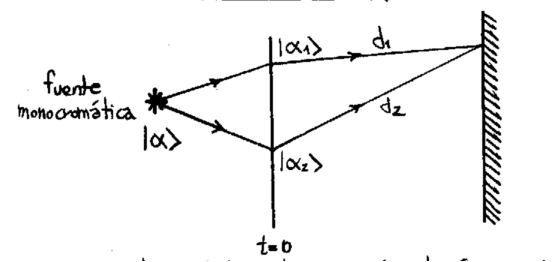
\includegraphics[width=0.6\textwidth]{images/teo2_6.pdf}	 
	\end{center}
	\caption{}
\end{figure} 

Uso $\hat{H}$ de partículas libres.
\[
	\frac{1}{2} \Ket{\alpha} = \Ket{\alpha_1} = \Ket{\alpha_2}
\]
para $t>0$ se tiene 
\[
	\Ket{\tilde{\alpha_1}} = \euler^{ -i H t /\hbar } \Ket{\alpha_1} =
		\euler^{ -i E_\alpha t /\hbar } \Ket{\alpha_1}	
\]
\[
	\Ket{\tilde{\alpha_2}} = \euler^{ -i E_\alpha t /\hbar } \Ket{\alpha_2}	
\]

En la pantalla debe verse la interferencia de los dos estados solapados.
\[
	\Ket{\tilde{\alpha}} = \Ket{\tilde{\alpha_1}} + \Ket{\tilde{\alpha_2}} =
		\euler^{ -i E_\alpha \frac{d_1}{v} /\hbar } \Ket{\alpha_1} +
		\euler^{ -i E_\alpha \frac{d_2}{v} /\hbar } \Ket{\alpha_2}	
\]
\[
	\Ket{\tilde{\alpha}} = \frac{1}{2} \euler^{ -i E_\alpha \frac{d_1}{v} /\hbar } 
		| 1 + \euler^{ -i E_\alpha \frac{d_2-d_1}{v} /\hbar } | \Ket{\alpha_1}
\]
y si definimos
\[
	\beta=E_\alpha \frac{d_2-d_1}{v} /\hbar,
\]
resulta entonces
\[
	\Braket{\tilde{\alpha}|\tilde{\alpha}} = \frac{1}{4}| 1 +  \euler^{ -i E_\alpha \frac{d_2-d_1}{v} 
/\hbar } |^2 =
		\frac{1}{4}( (1+\cos\beta)^2 + \sin^2\beta ) =
			\frac{1}{2} + \frac{1}{2}\cos\left( \beta \right).
\]


Al partir el estado $\Ket{\alpha_1} $ y volver a unirlo en $\Ket{\alpha_1} + \Ket{\alpha_2}$ vemos una 
intensidad que 
dependa de la diferencia de camino.

\subsection{Cambio de cero del potencial}

En mecánica clásica la física de un problema no se ve afectada por un cambio de gauge.
Si movemos el cero de potencial, la situación física es la misma.
Veamos qué sucede en mecánica cuántica.
\[
	\Ket{\alpha,t,t_0} = \euler^{ -i (p^2/2m + V(x))(t-t_0)/\hbar} \Ket{\alpha,t_0}
\]
\[
	\Ket{\tilde{\alpha},t,t_0} = \euler^{ -i (p^2/2m + V(x) + V_0)(t-t_0)/\hbar} \Ket{\alpha,t_0}
\]
\[
	\Ket{\tilde{\alpha},t,t_0} = \euler^{ -i V_0(t-t_0)/2 }\Ket{\alpha,t,t_0}
\]
y entonces vemos que $\Ket{\tilde{\alpha},t}$ y $\Ket{\alpha,t}$ difieren en una fase, de manera que los 
valores de 
expectación no cambian (con $V_0$ constante).

\begin{figure}[htb]
	\begin{center}
	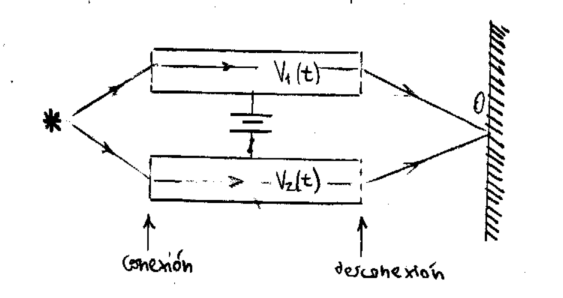
\includegraphics[width=0.6\textwidth]{images/teo2_7.pdf}	 
	\end{center}
	\caption{}
\end{figure} 

Este es un experimento ideal (pensado). Dentro de los cilindros hay campo nulo. Se varia el $V$ abriendo y 
cerrando la 
llave a la entrada y a la salida.
Se cambia la fase de las partículas inferiores respecto de las superiores, entonces habrá interferencia en 
$O$.

Clásicamente no hay variación,
\[
	\Delta \text{fase} = -\frac{i}{\hbar}\euler \int _{t_1}^{t_2} V_1(t) - V_2(t) dt = 
	-\frac{i}{\hbar}\euler \Delta V
\]

Lo que realmente cuenta es la diferencia de potencial $\Delta V$, la cual sí tiene sentido físico porque es 
independiente de la medida y porque pueden escribirse los campos en función de aquella.
\[
	E = - \Nabla\phi - \frac{1}{c}\dpar{\vb{A}}{t}
\]
\[
	H = \frac{1}{2m} \left( \vb{p} - \frac{\euler\vb{A}}{c}\right)^2 + \euler\phi 
\]
\[
	\dtot{H}{t} = \frac{1}{i\hbar}[x_i,H] = \frac{p_i  \euler A_i}{m}
\]

% =================================================================================================
\section{El propagador}
% =================================================================================================

Físicamente representa la proababilidad de transición entre autoestados por el paso del tiempo,
$ \Ket{x'}_{t_0} \longrightarrow \Ket{x''}_t$
\[
	\Braket{x''|\euler^{-iH(t-t_0)/\hbar}|x'} \equiv K(x',t; x, t_0)
\]
\[
	\Braket{x''| \alpha,t_0,t} = \Braket{x''|\euler^{-iH(t-t_0)/\hbar}|\alpha,t_0} 
\]
\[
	\Braket{x''| \alpha,t_0,t} = \int dx' \Braket{x''|\euler^{-iH(t-t_0)/\hbar}|x'}\Braket{x'|\alpha,t_0} 
\]
\[
	\Psi_{\alpha}(x'',t) = \int dx' K(x'',t; x',t) \Psi_{\alpha}(x',t)
\]

Podemos pensar que el propagador lleva la función de onda desde $t_0$ a $t$. Se puede escribir:
\[
	K(x',t; x, t_0) = \sum_{a'} \Braket{x''|a'} \Braket{a'|x'} \euler^{-iE_a(t-t_0)/\hbar}
\]
y metemos un observable $\hat{A}$ donde $[A,H]=0$ y $A\Ket{a'}=a\Ket{a'}$.

El propagador depende del potencial, pero no de la función de onda inicial. Se debe cumplir que:
\[
	\lim_{t\to t_0} K(x',t; x, t_0) = \delta^3(x''-x')
\]
\[
	K(x'',t; x, t_0) = \Braket{x''|\euler^{-iH(t-t_0)/\hbar}|a'} \Braket{a'|x'} =
		\sum_{a'} \Psi_{\Ket{a'}}(x'',t)\Braket{a'|x'}
\]
\[
	K(x'',t; x, t_0) = \sum_{a'} c_{a'}(x')\Psi_{\Ket{a'}}(x'',t)
\]
y entonces el propagador es una función de Green que satisface 
\[
	\left( -\frac{\hbar^2}{2m}\nabla^2 +V(x'') - i\hbar\dpar{}{t} \right)K(x',t; x, t_0) =
		- i\hbar \delta^3(x''-x') \delta(t-t_0)
\]
con $K(x'',t;x',t_0)=0 $ si $t<0$ que es la condición de contorno.

\subsection{El propagador de la partícula libre}

\[
	K(x'',t; x, t_0) = \int dp' \Braket{x''|\euler^{-ip^2(t-t_0)/2m\hbar}|p'} \Braket{p'|x'} 
\]
\[
	= \int dp' \euler^{-ip'^{2}(t-t_0)/2m\hbar} \Braket{x''|p'} \Braket{p'|x'} =
	\frac{1}{2\pi\hbar} \int dp' \euler^{-ip'^{2}(t-t_0)/2m\hbar} \euler^{-ip'(x'-x'')/\hbar}
\]
y entonces el propagador de una partícula libre es
\[
	K(x'',t; x, t_0) = \sqrt{ \frac{m}{2\pi\hbar(t-t_0)} } \euler^{i\frac{m(x''-x')^2}{2\hbar(t-t_0)}}
\]

También se puede escribir el propagador en la representación de Heisenberg,
\[
	\Braket{x''|\euler^{-iH(t-t_0)/\hbar}|x'} = \Bra{x''}\euler^{-iHt/\hbar} \euler^{iHt_0/\hbar}\Ket{x'}=
		\Braket{x'',t|x',t_0}
\]
\[
	K(x'',t;x',t_0) = \Braket{x'',t | x',t_0}.
\]

El propagador cumple con la propiedad de composición (como el $U(t,t_0)$), es decir:
\[
	K(x'',t; x, t_0) = K(x'',t; x, t_1)K(x'',t_1; x, t_0) \qquad t>t_1>t_0
\]

% =================================================================================================
\section{Integrales de camino de Feynmann}
% =================================================================================================

Consideramos una partícula yendo de $(x_1,t_1)$ a $(x_N,t_N)$. Dividimos el tiempo 
\[
	\delta t = \frac{t_N-t_1}{(N-1)}
\]
y queremos ver la amplitud de transición desde el estado 1 al $N$.

\begin{figure}[htb]
	\begin{center}
	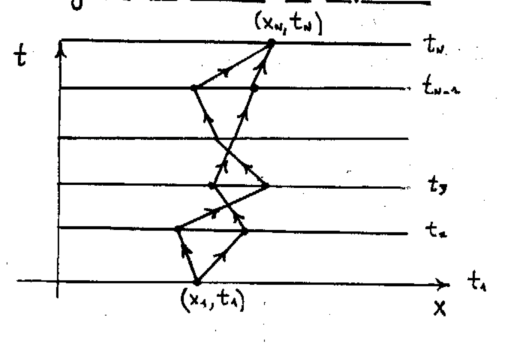
\includegraphics[width=0.6\textwidth]{images/teo2_8.pdf}	 
	\end{center}
	\caption{}
\end{figure} 

\[
	\braket{x_N,t_N|x_1,t_1} = \int dx_{N-1}\int dx_{N-2} \; ...\int dx_2
	\Braket{x_N,t_N|x_{N-1},t_{N-1}} ...\Braket{x_2,t_2|x_1,t_1}
\]

Se puede pensar como que estamos sumando sobre todos los posibles caminos entre $(x_1,t_1)$ y $(x_N,t_N)$ 
fijos. En mecánica clásica teníamos un solo camino, el que minimizaba la acción $S$
\[
	\delta \int_{t_1}^{t_2} \Lag dt = \delta S = 0
\]
pero en cambio en mecánica cuántica todos los caminos aportan. En un libro de Dirac, Feymann lee 
\[
	\Braket{x_2,t_2|x_1,t_1} \; \text{corresponde a} \; \euler^{i\int_{t_1}^{t_2}\Lag/\hbar dt}
\]
Definiremos
\[
	S_{(n,n-1)}\equiv \int_{t_{n-1}}^{t_n}\Lag(x,\dot{x}) dt
\]
Luego para considerar la suma sobre todos los segmentillos a lo largo de un camino tendremos
\[
	\prod_{n=2}^N \euler^{i/\hbar S(n,n-1)} = \euler^{i/\hbar \prod_{n=2}^N S(n,n-1)} = \euler^{iS(N,1)/\hbar}
\]
y hay que considerar TODOS los posibles caminos 
\[
	\propto \sum_{caminos} \euler^{i/\hbar S(N,1)} 
\]
cuando $\hbar \to 0$ las trayectorias contribuyen con una cantidad que oscila loca y violentamente. Tienden a 
la cancelación para caminos aledaños. Por el $\hbar \sim 0$ la fase es grande y entonces se cancelan.
Esto no ocurre cerca del camino (real) que cumple 
\[
	\delta S(N,1) = 0
\]
Para trayectorias cercanas la $\Delta fase$ no es grande y hay interferencia constructiva.
Para un $\delta t$ infinitesimal es 
\[
	\Braket{x_n,t_n|x_{n-1},t_{n-1}} = N \euler^{iS(n,n-1)/\hbar}
\]
\[
	S(n,n-1) = \int_{t_{n-1}}^{t_n} \left( \frac{m}{2}\dot{x}^2 - V(x)\right) dt \approx
	\int_{t_{n-1}}^{t_n} \left( \frac{m}{2} \frac{(x_n-x_{n-1})^2}{\delta t^2} - 
	V\left(\frac{x_n+x_{n-1}}{2}\right)\right)  dt
\]
donde la última expresión es a orden 1 (pues $\delta t \sim 0$).
\begin{figure}[htb]
	\begin{center}
	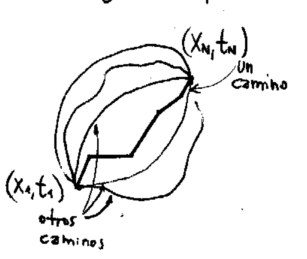
\includegraphics[width=0.6\textwidth]{images/teo2_9.pdf}
	\end{center}
	\caption{}
\end{figure} 

Consideremos, por ejemplo, una partícula libre, entonces $V=0$ de modo que resolviendo 
\[
	\Braket{x_n,t_n|x_{n-1},t_{n-1}} = N \euler^{im(x_n - x_{n-1})/2\hbar\delta t}
\]
Esto no es otra cosa que el propagador de una partícula libre. Para un $\Delta t$ finito será 
\[
	\Braket{x_n,t_n|x_1,t_1}  = \lim_{N\to\infty} \left(\frac{m}{i2\pi\hbar\delta t}\right)^{(N-1)/2}
	\int dx_{n-1}\int dx_{n-2} \; ... \int dx_2 \prod_{n=2}^N \euler^{i S(n,n-1)/\hbar}
\]
\[
	\Braket{x_n,t_n|x_1,t_1}  = \int_{x_1}^{x_n} D[x(t)] \euler^{i \int _{t_1}^{t_n} \Lag(x,\dot{x})/\hbar} dt
\]
siendo esta última la integral de camino de Feynmann.

En base a éstas Feynamn desarrolla una formulación equivalente de la mecánica cuántica que utiliza los 
conceptos de:
\begin{enumerate}
 \item Superposición
 \item Composición de la transición
 \item Límite clásico con $\hbar \to 0$
\end{enumerate}

Estas integrales contienen toda la información del sistema cuántico, aunque no sea sencillo extraerla.

Consideremos un propagador de $(x',0) \to (x',t)$
\[
	G(t) = \int dx' K(x',t ; x', 0) = \int dx' \Braket{x'|\euler^{-i Ht/\hbar}|x'}
\]
\[
	G(t) = \sum_{a'} \int dx' \Braket{x'|\euler^{-i Ht/\hbar}|a'}\Braket{a'|x'} =
		\sum_{a'} \euler^{-i E_{a'}t/\hbar} \int dx' \Braket{x'|a'}\Braket{a'|x' }
\]
\[
	G(t) = \sum_{a'} \euler^{-i E_{a'}t/\hbar} \int dx' |\Braket{x'|a'}|^2 = \sum_{a'} \euler^{-i E_{a'}t/\hbar} 
\]
que es reminiscencia de la función de partición de mecánica estadística. Tomando Laplace-Fourier 
\[
	\tilde{G}(E) = -i \int dE \frac{G(t)}{\hbar} \euler^{i E t/\hbar} = \sum_{a'} \frac{1}{E-E_{a'}}
\]
y el espectro de autoenergías son los polos de $\tilde{G}(E)$.

La expresión 
\[
	\Braket{x,t|x_1,t_1} \equiv \text{Integral de camino de Feynmann}
\]
satisface la ecuación de Schrödinger y es una alternativa a la formulación de la cuántica usual.


% \bibliographystyle{CBFT-apa-good}	% (uses file "apa-good.bst")
% \bibliography{CBFT.Referencias} % La base de datos bibliográfica

\end{document}

	
% 		\documentclass[10pt,oneside]{CBFT_book}
	% Algunos paquetes
	\usepackage{amssymb}
	\usepackage{amsmath}
	\usepackage{graphicx}
	\usepackage{libertine}
	\usepackage[bold-style=TeX]{unicode-math}
	\usepackage{lipsum}

	\usepackage{natbib}
	\setcitestyle{square}

	\usepackage{polyglossia}
	\setdefaultlanguage{spanish}
	



	\usepackage{CBFT.estilo} % Cargo la hoja de estilo

	% Tipografías
	% \setromanfont[Mapping=tex-text]{Linux Libertine O}
	% \setsansfont[Mapping=tex-text]{DejaVu Sans}
	% \setmonofont[Mapping=tex-text]{DejaVu Sans Mono}

	%===================================================================
	%	DOCUMENTO PROPIAMENTE DICHO
	%===================================================================

\begin{document}





% \bibliographystyle{CBFT-apa-good}	% (uses file "apa-good.bst")
% \bibliography{CBFT.Referencias} % La base de datos bibliográfica

\end{document}

	
		\documentclass[10pt,oneside]{CBFT_book}
	% Algunos paquetes
	\usepackage{amssymb}
	\usepackage{amsmath}
	\usepackage{graphicx}
	\usepackage{libertine}
	\usepackage[bold-style=TeX]{unicode-math}
	\usepackage{lipsum}

	\usepackage{natbib}
	\setcitestyle{square}

	\usepackage{polyglossia}
	\setdefaultlanguage{spanish}
	

	\everymath{\displaystyle}

	\usepackage{CBFT.estilo} % Cargo la hoja de estilo

	% Tipografías
	% \setromanfont[Mapping=tex-text]{Linux Libertine O}
	% \setsansfont[Mapping=tex-text]{DejaVu Sans}
	% \setmonofont[Mapping=tex-text]{DejaVu Sans Mono}

	%===================================================================
	%	DOCUMENTO PROPIAMENTE DICHO
	%===================================================================

\begin{document}

% =================================================================================================
\chapter{Introducción al momento angular (rotaciones)}
% =================================================================================================

El operador $\hat{L}$ será el encargado de realizar las rotaciones. Por el álgebra visto en la mecánica 
clásica sabemos que, dado un vector \vb{v} y una matriz ortogonal $R$ se tiene
\[
	\vb{v}' = R \vb{v} \qquad \text{con} \quad |\vb{v}'|=|\vb{v}|
\]
y 
\[
	|\vb{v}|^2 = V^t V = (V^t R^t) (R V) \qquad \text{pues} \quad R^tR=RR^t = \mathbb{1}
\]
puesto que es una matriz ortogonal. Luego se cumplen 
\[
	clausura	
\]
el producto de dos matrices ortogonales es otra matriz ortogonal
\[
	asociatividad
\]
\[
	E identidad
\]
\[
	E inversa
\]

\subsection{No conmutatividad de las rotaciones clásicas}

Las rotaciones finitas no conmutan. Luego, el grupo de las rotaciones será un grupo abeliano
\[
	R_z(\varphi) = \begin{pmatrix}
	\cos(\varphi) & -\sin(\varphi) & 0 \\
	\sin(\varphi) & \cos(\varphi) & 0 \\
	0 & 0 & 1
	\end{pmatrix}
\]
\[
	R_x(\varphi) = \begin{pmatrix}
	1 & 0 & 0 \\
	0 & \cos(\varphi) & -\sin(\varphi) \\
	0 & \sin(\varphi) & \cos(\varphi)
	\end{pmatrix}
\]
\[
	R_y(\varphi) = \begin{pmatrix}
	\cos(\varphi) & 0 & \sin(\varphi) \\
	0 & 1 & 0 \\
	-\sin(\varphi) & 0 & \cos(\varphi)
	\end{pmatrix}
\]

\begin{figure}[htb]
	\begin{center}
	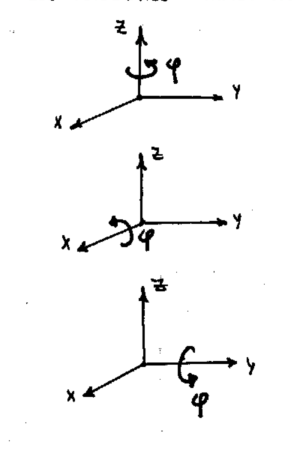
\includegraphics[width=0.6\textwidth]{images/teo2_10.pdf}
	\end{center}
	\caption{}
\end{figure} 

Si reemplazamos $\cos(\epsilon) \approx 1 - \epsilon^2/2$ y $\sin(\epsilon) \approx \epsilon$ hasta orden dos.
Se puede ver que las rotaciones, en torno a ejes diferentes, sólo conmutan a orden uno $(\epsilon)$ de manera 
que una rotación infinitesimal $d\varphi$ conmuta pero una rotación finita $\varphi$ no lo hace.

% =================================================================================================
\section{Rotaciones cuánticas}
% =================================================================================================

Para las rotaciones cuánticas se pedirá
\[
	D,
\]
rotación infinitesimal o bien
\[
	D,
\]
para rotación finita. Donde $\hat{D}$ es el operador de las rotaciones y $\hat{J}$ es un momento angular 
general. Se postula de esta forma para que $\hat{D}$ cumpla las mismas propiedades que $R$ y la relación de 
conmutación
\[
	R_x R_y - R_y R_x = R_z (\epsilon^2) - \mathbb{1}
\]
\[
	D
\]
de modo que la cuenta lleva a  
\[
	J_x
\]
la cual generalizando se llega a 
\[
	[J_i,J_j] = i \hbar \epsilon_{ijk} J_k
\]
que son las relaciones de conmutación generales para momento angular $\hat{J}$.

Para sistemas de spín $1/2$ es 
\[
	D(\hat{n},\phi) \equiv \euler^{-i/\hbar \vb{S}\cdot\hat{n} }
\]
Se puede ver que ante rotaciones cuánticas $D(\hat{n},\phi)$ los valores de expectación transforman como 
vectores
\[
	=
\]

En general $\vb{J} = (J_x, J_y, J_z)$ se transforma como vector y entonces $\hat{J}$ es un operador vectorial.
Para spín $1/2$ es
\[
	\Ket{alpha} =
\]
\[
	D
\]
\[
	D
\]
Si $\phi=2\pi$ (cosa que debiera dejar al ket incólume) se tiene 
\[
	D
\]

Luego, esto es una muestra del carácter no-clásico del spin; una vuelta completa le cambia el signo al ket 
pero notemos cuidadosamente que el valor de expectación -- que es algo físico -- no varía. Esto muestra que 
el ket no puede tener sentido físico.

\subsection{Angulos de Euler}

Se define una serie de rotaciones 
\[
	1 2 3
\]
lo cual equivale a
\[
	R() = 
\]
\[
	\euler
\]

Pero desconozco cómo operar en los ejes móviles $z',y'$
\[
	R_{y'}(\beta) =
\]
\[
	R_{z'}(\gamma) =
\]
\[
	R() =
\]
Rotación equivalente a [1] pero para ejes fijos, puesto que en mecánica cuántica sabemos rotar en torno a 
ejes fijos.

Los ángulos de Euler son la caracterización de una rotación general en 3D.

Entonces nuestra rotación en 3D cuántica será:
\[
	D() =
\]

\subsection{Autoestados y autovalores de J}

Partimos de 
\[
	[] = 
\]
y
\[
	J^2 = , [J^2,J] = 0
\]
siendo la última muy importante y probándose por evaluación directa. Lleva a 
\[
	[J^2,J_i^n] = 0 \qquad \text{con} \; i=x,y,z \; n\in\mathbb{N}
\]

Se eligen $J^2, J_z$ como observables que conmutan 
\[
	J^2
\]

Definiremos los operadores de subida y de bajada
\[
	J_{\pm} \equiv J_x \pm J_y
\]
que verifican 
\[
	[]
\]
Entonces se tiene 
\[
	J^2() \longrightarrow 
\]
\[
	(J_z) \longrightarrow
\]

\[
	J_{\pm} \Ket{a,b} = C_{\pm} \Ket{a,b\pm\hbar}
\]
\[
	J_+
\]
sube el $J_z$ en una unidad de $\hbar$ o bien baja el $J_z$ en una unidad de $\hbar$.
\[
	J_+J_- =  ,
\]
\[
	J^2 = ,  
\]
\[
	\Braket{a,b|J^2 - J^2_z|a,b} = 
\]
\[
	(a-b^2)\Braket{a,b|a,b} = , a \geq b^2
\]
hay cota para $b$.
Como no puede seguir subiendo debe dar el ket nulo 
\[
	= 0
\]
\[
	= 0
\]
pero 
\[
	J_-J_+
\]
\[
	= 0	\qquad a = b_m(b_m-\hbar)
\]
tiene solución 
\[
	b_M - B_m = - \hbar
\]
pero esto es absurdo.

Luego,
\[
	\Ket{a,b_m} \longrightarrow \Ket{a,b_M}
\]
y como $J_+$ sube de a un $\hbar$ será
\[
	b_M = b_m + n\hbar
\]
y entonces
\[
	b_M = \frac{n\hbar}{2} = \frac{n}{2} \hbar = j \hbar
\]
y se da que $j$ es entero o semientero.

Definiremos 
\[
	b_M \equiv j \hbar \qquad a \equiv j (j+1) \hbar^2 \qquad -j\hbar \leq b \leq j\hbar
\]
pero como $b/\hbar = m$
\[
	b_M \equiv j \hbar \qquad a \equiv j (j+1) \hbar^2 \qquad -j \leq m \leq j
\]
\[
	m = (-j,-j+1,-j+2,...,j-1,j) \qquad 2j+1 \text{valores de} \; m
\]
\[
	J^2 \Ket{j,m} = j( j+1 )\hbar^2\Ket{j,m} \qquad J_z \Ket{j,m} = m \hbar \Ket{j,m}
\]

\subsection{La normalización de $J_\pm$}

\[
	J_+
\]
\[
	\Braket{j,m|J_-J_+|j,m} = 
\]
\[
	c_+ = 
\]
\[
	\Braket{j,m|J_+J_-|j,m} = 
\]
\[
	c_- =
\]
\[
	J_+
\]

\subsection{Elementos de matriz de $J^2, J_z, J_+$}

Asumiendo normalización de $\Ket{j,m}$ se tiene 
\[
	\Braket{} = 
\]
\[
	=
\]

\subsection{Elementos de matriz de $\mathcal{D}(R)$}

Ahora queremos ver cual es la forma de los elementos de matriz de $\mathcal{D}(R)$
\[
	\mathcal{D}(R) =
\]
siendo que $\mathcal{D}(R)$ tiene por efecto rotar el sistema físico.
Lo primero que hay que notar es que 
\[
	\propto \delta_{jj'}
\]
porque $[J^2,J_i]=0$ y entonces $[J^2,J_i^n]=0$ y 
\[
	D
\]
y 
\[
	D
\]
es una matriz para cada $j$ fijo con $\{ (2j+1)\times(2j+1)=\text{dimensión}\}$
\[
	D
\]
pero las rotaciones no cambian el $j$, $\mathcal{D}(R)$ conecta estados con la misma $j$ y $\mathcal{D}(R) 
\in (2j+1)\times(2j+1)$ 
\[
	D
\]

La matriz de $\mathcal{D}(R)$ (no caracterizada por un único $j$) puede ponerse en forma diagonal por bloques:


con cada bloque de $(2j+1)\times(2j+1)$ , pero siendo cada bloque irreducible. Las matrices de rotación con 
$j$ fijo forman un grupo. $\mathcal{D}_{m'm}^{(j)}(R)$ son los elementillos de la matriz.
\[
	\Ket{j,m} \longrightarrow
\]

\subsection{Forma explícita del operador $\mathcal{D}(R)$}

Los ángulos de Euler permitieron caracterizar la rotación más general. Entonces 
\[
	D
\]
\[
	D
\]

En los $d_{m'm}^{(j)}$ está la dificultad de la cuenta.

% =================================================================================================
\section{Formalismo de spinores de Pauli}
% =================================================================================================

Apropiado para trabajar con sistemas de spín $1/2$. Estos sistemas son casos particulares de momento angular,
\[
	j = 1/2 \qquad m=-\frac{1}{2},+\frac{1}{2}
\]
y se definen los spinores $\chi_\pm$ como
\[
	\Ket{+} \equiv  \begin{pmatrix} 1 \\ 0  \end{pmatrix} \equiv  \chi_+ \qquad \qquad
	\Ket{-} \equiv  \begin{pmatrix} 0 \\ 1  \end{pmatrix} \equiv  \chi_-
\]
\[
	\Ket{\alpha} = \begin{pmatrix}   \Braket{+|\alpha} \\ \Braket{-|\alpha}  \end{pmatrix}
\]
\[
	\Bra{\alpha} = \begin{pmatrix}  \; \Braket{+|\alpha} \quad \Braket{-|\alpha} \;  \end{pmatrix}
\]

Para spín $1/2$ podemos tomar $\vb{J} = \vb{S}$ por la analogía de las relaciones de conmutación.
A su vez 
\[
	\vb{S} = \frac{\hbar}{2} \vec{\sigma} \qquad \text{con} \qquad \vec{\sigma} \equiv 
	\begin{pmatrix} \; \sigma_x, \sigma_y, \sigma_z \; \end{pmatrix}
\]
que es una especie de vector 
\[
	\vec{\sigma}  =
	\begin{bmatrix}
	 \begin{pmatrix} 0 & 1 \\ 1 & 0 \end{pmatrix}, \begin{pmatrix} 0 & -i \\ i & 0 \end{pmatrix},
	 \begin{pmatrix} 1 & 0 \\ 0 & -1 \end{pmatrix} 
	\end{bmatrix}
\]
Luego esta equivalencia provee expresión de los operadores $S_i$ en términos de matrices de $2\times 2$, así:
\[
	\frac{i}{2}[ J_- - J_+] = J_y = S_y = \frac{\hbar}{2} \sigma_y
\]
siendo que los $J_y$ y $S_y$ actúan sobre kets y el $\sigma$ sobre spinores.

Las matrices de Pauli cumplen las propiedades básicas siguientes 
\[
	\sigma^2_i = \mathbb{1} \qquad \sigma_i^\dagger = \sigma_i
\]
\[
	[ \sigma_, \sigma_j ] = i2\varepsilon_{ijR}\sigma_R \qquad \{\sigma_, \sigma_j \}= \delta_{ij}
\]
\[
	\sigma_i^n = \begin{cases} \mathbb{1} \quad n \; \text{par} \\ \sigma_i \quad n \; \text{impar} 
\end{cases}
\]
\[
	\Ket{+} \equiv \Ket{j=1/2 , m = 1/2} \qquad \Ket{-} \equiv \Ket{j=1/2 , m = -1/2} 
\]
\[
	(\vec{\sigma}\cdot\vb{a})(\vec{\sigma}\cdot\vb{b}) = 
		(\vb{a}\cdot\vb{b}) + i \vec{\sigma}\cdot(\vb{a}\times\vb{b})
\]

\subsection{Aplicación a las rotaciones}

\[
	\mathcal{D}(\hat{n},\phi) = \euler^{-i \vb{J}\cdot\hat{n}\phi/\hbar} = \euler^{-i\vec{\sigma}\cdot\hat{n}\phi/2}
\]
pero 
\[
	(\vec{\sigma}\cdot\hat{n})^n = \begin{cases}
	                                \vec{\sigma}\cdot\hat{n} \qquad n \; \text{impar} \\
	                                \mathbb{1} \qquad \quad \; n \; \text{par} 
	                               \end{cases}
\]
\[
	\euler^{-i\vec{\sigma}\cdot\hat{n}\phi/2} = 1 - i\vec{\sigma}\cdot\hat{n} \:\frac{\phi}{2} - 
	\frac{1}{2!} (\vec{\sigma}\cdot\hat{n})^2\left(\frac{\phi}{2}\right)^2 + 
	\frac{i}{3!} (\vec{\sigma}\cdot\hat{n})^3\left(\frac{\phi}{2}\right)^3 - ...
\]
\[
	\mathcal{D}(\hat{n},\phi) = \euler^{-i\vec{\sigma}\cdot\hat{n}\phi/2} =
	\mathbb{1}\cos\left(\frac{\phi}{2}\right) - i\vec{\sigma}\cdot\hat{n}\sin\left(\frac{\phi}{2}\right)
\]
es el operador de rotación para sistemas de spin $1/2$ (donde $\mathbb{1} \in 2\times 2$). Con esta expresión podemos 
evaluar 
$d^{j=1/2}_{m'm}(\beta)$
\[
	d^{1/2}(\beta) = \begin{pmatrix}
	     \cos(\beta/2) & -\sin(\beta/2)\\
	     \sin(\beta/2) & \cos(\beta/2)
	    \end{pmatrix}
\]
donde hemos usado los resultados 
\[
	\cos(x) = \sum_{n=0}^\infty \frac{(x)^{2n+1}}{(2n+1)!}(-1)^n \qquad 
		\sin(x) = \sum_{n=0}^\infty \frac{(x)^{2n}}{(2n)!}(-1)^n
\]

En el caso general el operador de rotación para sistemas de spin $1/2$ lucirá:
\[
	\begin{matrix} \qquad\qquad \Ket{+} \qquad\qquad\qquad\qquad \Ket{-} \end{matrix}
\]
\[
	\mathcal{D}^{j=1/2} (\alpha,\beta,\gamma) = \begin{pmatrix}
	        \euler^{-\frac{i}{2}(\alpha + \gamma)} \cos\left(\frac{\beta}{2}\right) & 
			- \euler^{-\frac{i}{2}(\alpha - \gamma)} \sin\left(\frac{\beta}{2}\right) \\
	        \euler^{-\frac{i}{2}(\gamma -\alpha )} \sin\left(\frac{\beta}{2}\right) & 
			\euler^{\frac{i}{2}(\alpha + \gamma)} \cos\left(\frac{\beta}{2}\right)
	       \end{pmatrix} 
	       \begin{matrix} \Ket{+} \\ \\  \Ket{-} \end{matrix}
\]

\subsection{Ejemplo}

\[
	d^{1/2}(\pi/2) = \begin{pmatrix}
	                  \sqrt{2}/2 & -\sqrt{2}/2 \\
	                  \sqrt{2}/2 & \sqrt{2}/2
	                 \end{pmatrix}
\]
de manera que 
\[
	d^{1/2}(\pi/2)\chi_{+} = \frac{\sqrt{2}}{2}\begin{pmatrix} 1 & -1 \\  1 & 1 \end{pmatrix}
	                                           \begin{pmatrix}  1 \\ 0  \end{pmatrix} 
				= \frac{\sqrt{2}}{2} \begin{pmatrix}  1 \\ 1 \end{pmatrix} 
\]
\[
	d^{1/2}(\pi/2)\chi_{+} = \frac{\sqrt{2}}{2} (\chi_+ + \chi_- )  = \frac{1}{2} \left( \Ket{+} + \Ket{-} \right)
\]
\[
	d^{1/2}(\pi/2)\chi_{+} = \Ket{S_x ; + }
\]
Este resultado es intuitivamente lógico.


\subsection{Rotaciones en sistemas con $j=1$}

Ahora tenemos 
\[
	j=1 \qquad m = -1,0,1
\]
recordando $J_y$ en términos de escaleras
\[
	J_y = \frac{J_+ - J_i}{2i}
\]
de modo que 
\[
	\begin{matrix} \quad \Ket{1\;1} \quad \Ket{1\;0} \quad \Ket{1\;-\kern-1mm 1} \end{matrix}
\]
\[
	J_y = \frac{i\hbar}{\sqrt{2}} \begin{pmatrix}
	                               \quad 0 & \quad -1 \quad & 0 \quad \\
	                               \quad 1 & \quad 0 \quad & -1 \quad \\
	                               \quad 0 & \quad 1 \quad & 0 \quad
	                              \end{pmatrix} 
	     \begin{matrix}  \Ket{1\;1} \\ \Ket{1\;0} \\ \Ket{1\;-\kern-1mm 1} \end{matrix}
\]
\[
	\euler^{-i\frac{J_y}{\hbar}\beta} = 1 + -\frac{J_y}{\hbar}\beta + 
		(-i)^2\left(\frac{J_y}{\hbar}\beta\right)^2\frac{1}{2!} + 
		(-i)^3\left(\frac{J_y}{\hbar}\beta\right)^3\frac{1}{3!} + ...
\]
\[
	\euler^{-i\frac{J_y}{\hbar}\beta} = 1 - \frac{J_y}{\hbar}\beta -
		\frac{1}{2!} \left(\frac{J_y}{\hbar}\beta\right)^2 -
		\frac{i}{3!}\left(\frac{J_y}{\hbar}\beta\right)^3 + ...
\]
\[
	\left( \frac{J_y}{\hbar} \right)^n = \begin{cases}
	                                      \left( \frac{J_y}{\hbar} \right) \quad n \; \text{impar} \\
	                                      \left( \frac{J_y}{\hbar} \right)^2 \quad n \; \text{par}
	                                     \end{cases}
\]
\[
	\euler^{-i\frac{J_y}{\hbar}\beta} = 1 -  \left( \frac{J_y}{\hbar} \right)^2 (1-\cos(\beta)) -
	i \left( \frac{J_y}{\hbar} \right) \sin(\beta)  = d^{j=1}(\beta)
\]
acá lo vemos como operador (es notación), $d_{m'm}^{j=1}(\beta)$ simboliza la matriz
\[
	\begin{matrix} \Ket{1\;1} \qquad\qquad\quad \Ket{1\;0} \qquad\qquad \Ket{1\;-\kern-1mm 1} \end{matrix}
\]
\[
	d^{j=1}(\beta) =
	\begin{pmatrix}
	\displaystyle \frac{1}{2}( 1 + \cos(\beta)) & -\frac{1}{\sqrt{2}}\sin(\beta) & \frac{1}{2}( 1 - 
\cos(\beta) ) \\
	\displaystyle{\frac{1}{\sqrt{2}}\sin(\beta)} & \cos(\beta) & -\frac{1}{\sqrt{2}}\sin(\beta) \\
	\displaystyle{\frac{1}{2}(1 - \cos(\beta))} & \frac{1}{\sqrt{2}}\sin(\beta) & \frac{1}{2}  ( 1 + 
\cos(\beta) )
	\end{pmatrix} \begin{matrix} \Ket{1\;1} \\ \\ \Ket{1\;0} \\ \\ \Ket{1\;-\kern-1mm 1} \end{matrix}
\]

% =================================================================================================
\section{Momento angular orbital}
% =================================================================================================

\[
	\vb{L} =
\]
verifica el álgebra de $\vb{J}$,
\[
	[]
\]
Consideremos ahora una rotación en torno a $z$, en un $\delta\phi$,
\[
	() =
\]
\[
	() = 
\]
esto es una traslación en $\hat{x},\hat{y}$,
\[
	(1-i\frac{L_z}{\hbar}\delta\phi) \Ket{x',y',z'} = \Ket{}
\]

Esta traslación es debida a una rotación infinitesimal en $\delta\phi$ torno a $z$ entonces genera las 
rotaciones clásicas en torno a $z$.
\[
	\Psi 
\]
\[
	\Psi
\]

Podemos hallar una expresión para $L_z$ en esféricas:
\[
	\Braket{r,\theta,\varphi||\alpha}
\]
identificamos 
\[
	= 
\]
operador $L_z$ en esféricas

Usando 
\[
	L^2 = 
\]
\[
	\Braket{L^2}
\]
\[
	L^2 = -\hbar^2 r^2 \nabla^2_{\theta,\varphi}
\]
donde $\nabla^2_{\theta,\varphi}$ es la parte angular del laplaciano en coordenadas esféricas.
Esto puede obtenerse también partiendo de 
\[
	L^2 = \vb{x}^2\vb{p}^2 - (\vb{x}\cdot\vb{p})^2 + i\hbar \vb{x}\cdot\vb{p}
\]

Sea un $H$ de partícula, sin spín, sujeta a potencial simétricamente esférico. Sabemos que la función de onda 
$\Psi_\alpha(\vb{r}')$ es separable en coordenadas esféricas, entonces:
\[
	\Braket{|} = 
\]
\[
	\Braket{|} = 
\]

Cuando el H es esféricamente simétrico (como en un potencial central) se tiene 
\[
	[] = [] = 0
\]

Trabajaremos solamente en la parte angular  $\Ket{\theta,\varphi} \equiv \Ket{\hat{n}}$
\[
	\Braket{\hat{n}|\ell,m} =
\]
que es la amplitud de hallar $\Ket{\ell,m}$ en la dirección $\hat{n}$.

Podemos vincular ahora los armónicos esféricos con los autoestados de $L_z,L^2$
\[
	L_z
\]
\[
	L^2
\]
\[
	=
\]
Entonces, con la ortogonalidad
\[
	\longrightarrow
\]
y con la completitud 
\[
	\longrightarrow
\]
de manera que llegamos a 
\[
	\int \int 
\]

Podemos hallar una expresión para 
\[
	= 0
\]
\[
	\Rightarrow
\]

Luego usamos $L_-$ para hallar sucesivamente los demás $Y^m_\ell$
\[
	=
\]
y por este camino se llega a 
\[
	Y
\]
con 
\[
	\qquad 
\]

En el caso de momento angular orbital $\ell$ no puede ser semientero porque entonces $m$ sería semientero y 
en una vuelta de $2\pi$
\[
	\euler^{im2\pi} = -1
\]	

Además,
\[
	\text{(no hay signo menos)}
\]


% \bibliographystyle{CBFT-apa-good}	% (uses file "apa-good.bst")
% \bibliography{CBFT.Referencias} % La base de datos bibliográfica

\end{document}

	
		\documentclass[10pt,oneside]{CBFT_book}
	% Algunos paquetes
	\usepackage{amssymb}
	\usepackage{amsmath}
	\usepackage{graphicx}
	\usepackage{libertine}
	\usepackage[bold-style=TeX]{unicode-math}
	\usepackage{lipsum}

	\usepackage{natbib}
	\setcitestyle{square}

	\usepackage{polyglossia}
	\setdefaultlanguage{spanish}
	



	\usepackage{CBFT.estilo} % Cargo la hoja de estilo

	% Tipografías
	% \setromanfont[Mapping=tex-text]{Linux Libertine O}
	% \setsansfont[Mapping=tex-text]{DejaVu Sans}
	% \setmonofont[Mapping=tex-text]{DejaVu Sans Mono}

	%===================================================================
	%	DOCUMENTO PROPIAMENTE DICHO
	%===================================================================

\begin{document}

% =================================================================================================
\chapter{Armónicos esféricos como matrices de rotación}
% =================================================================================================
Se pueden hallar autoestados de dirección $\Ket{\hat{n}}$ rotando el $\Ket{\hat{z}}$,
\[
	\hat{n} = \mathcal{D}(R) \Ket{\hat{z}}
\]

\begin{figure}[!htb]
	\begin{center}
	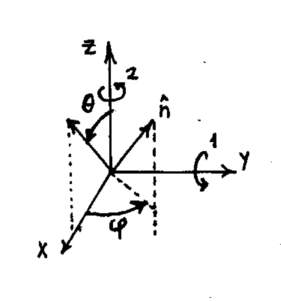
\includegraphics[width=0.25\textwidth]{images/teo2_12.pdf}
	\end{center}
	\caption{.}
\end{figure} 
Necesitamos aplicar $\mathcal{D}(R)=\mathcal{D}(\alpha=\varphi,\beta=\theta,\gamma=0)$
\[
	\Ket{\hat{n}} = \sum_{m,\ell} \mathcal{D} (R) \Ket{\ell,m}\Braket{\ell,m|\hat{z}}
\]
\[
	\Braket{\ell,m'|\hat{n}} = \sum_{m,\ell} \Braket{\ell,m'|\mathcal{D} (R)| \ell,m}\Braket{\ell,m|\hat{z}}
\]
pero como la $\mathcal{D}(R)$ no conecta $\ell$ diferentes, se tiene 
\[
	\Braket{\ell,m'|\hat{n}} = \sum_{m} \mathcal{D}_{m'm}^\ell(R) \Braket{\ell,m|\hat{z}}	
\]
\[
	Y_\ell^{m'*}(\theta,\varphi) = \sum_m \mathcal{D}_{m'm}^\ell(R) Y_\ell^{m*} (\theta=0,\varphi \text{indet})
\]
pero como $\theta=0$ , $Y_\ell^m = 0$  con $m\neq 0$ se tiene 
\[
	\Braket{\ell,m|\hat{z}} = Y_\ell^{m*} (\theta=0,\varphi \text{indet}) \delta_{m0}
\]
\[
	\Braket{\ell,m|\hat{z}} = \sqrt{ \frac{2\ell +1}{4\pi} } \delta_{m0}
\]
\[
	Y_\ell^{m'*}(\theta,\varphi) = \sqrt{ \frac{2\ell +1}{4\pi} }
	\mathcal{D}_{m'0}^\ell (\alpha=\varphi,\beta=\theta,\gamma=0)
\]
la matriz de rotación en este caso es un armónico esférico.

La $\Psi$ tiene la misma simetría que el potencial.

% =================================================================================================
\section{Suma de momentos angulares}
% =================================================================================================

\subsection{Dos momentos de spín $1/2$}

Sean dos estados de spín $1/2$
\[
	\vb{S} = \vb{S}_1 + \vb{S}_2 \equiv \vb{S}_1 \otimes \mathbb{1}_2 + \mathbb{1}_1\otimes \vb{S}_2
\]
en cada espacio valen las relaciones usuales de conmutación 
\[
	[ S_{1/2i},S_{1/2j}] = i\hbar\epsilon_{ijk}S_{1/2k}, \qquad  [S_{1i},S_{2j}] = 0
\]
donde el último indica que operadores de espacios diferentes conmutan.

Un estado general es 
\[
	\Ket{S_1,m_1} \otimes \Ket{S_2,m_2} \equiv \Ket{S_1, S_2;m_1,m_2}
\]
Hay cuatro estados
\[
	\begin{matrix} S_1 \quad S_2 \quad\quad m_1 \quad m_2 \end{matrix}
\]
\[
	\begin{matrix}
	&\Ket{1/2, 1/2 ; \phantom{-}1/2, \phantom{-}1/2} \\
	&\Ket{1/2, 1/2 ; \phantom{-}1/2, -1/2} \\
	&\Ket{1/2, 1/2 ; -1/2, -1/2} \\
	&\Ket{1/2, 1/2 ; -1/2, \phantom{-}1/2}
	\end{matrix}
\]	
\[	
	\begin{matrix} S_1 \quad S_2 \quad\quad S_{1z} \quad S_{2z}  \end{matrix}
\]
que corresponden a los operadores $S_ 1^2, S_2^2, S_{1z}, S_{2z}$ que conmutan (son un CCOC).

Podemos elegir otras base de operadores que comutan que será: $S_ 1^2, S_2^2, S, S_{z}$, de modo que el estado 
general será
\[
	\Ket{S_1, S_2;S,m}
\]
Así tendremos
\[
	\begin{matrix} \qquad\qquad S_1 \quad S_2 \quad S \quad m \end{matrix}
\]
\[
	\begin{matrix}
	\text{Triplete}\begin{cases}	
	&\Ket{1/2, 1/2 \; ; \; 1, \phantom{-}1} \\
	&\Ket{1/2, 1/2 \; ; \; 1, \phantom{-}0} \\
	&\Ket{1/2, 1/2 \; ; \; 1, -1} \\
	\end{cases}
	\\
	\text{Singlete}\begin{cases}
	&\Ket{1/2, 1/2 \; ; \; 0, \phantom{-}0} \\
	\end{cases}		
	\end{matrix}	 
\]	
\[	
	\begin{matrix} \qquad\qquad S_1^2 \quad S_2^2 \quad S^2 \quad S_z  \end{matrix}
\]
y recordemos que $m_1+m_2=m$ y $s_1+s_2=s$
\[
	S^2 = (S_1 + S_2)^2  = S_1^2 + S_2^2 + 2\vb{S}_1\cdot\vb{S}_2 \qquad 
	S^2_z = (S_{1z} + S_{2z})^2  = S_{1z}^2 + S_{2z}^2 + 2S_{1z}\cdot S_{2z}
\]

Dada la repetición de $S_1,D_2$ se suelen identificar a las bases solamente 
\[
	\begin{cases}
	\{ \Ket{m_1,m_2} \} \\
	\{ \Ket{S,m} \}
	\end{cases}
\]
Además la base $\{ \Ket{m_1,m_2}\}$ se puede poner como 
\[
	+ \equiv + 1/2 \qquad\qquad - \equiv - 1/2
\]

\subsection{Cambio entre bases}

Podemos hallar a ojo que 
\[
	\cdot \Ket{++} = \Ket{1,1} \qquad \cdot \Ket{--} = \Ket{1,-1} 
\]
de manera que la única forma de tener $m=1$ es con los dos spines up y la única forma de tener $m=-1$ es con 
los dos 
spines down.

Se hallan los otros con el operador de bajada
\[
	S_- \equiv S_{1-} + S_{2-}
\]
y si descompongo $S_-$ en $S_{1-}$ y $S_{2-}$ para operar en $\Braket{s,m}$ se tiene 
\[
	S
\]
y ahora si opero con $S_-$,
\[
	S
\]

Luego
\[
	\Braket{00}
\]
y puedo usar ortonormalidad 
\[
	= 0 = \qquad \text{con} \; |a|^2 + |b|^2 = 1
\]
\[
	\cdot 
\]


\section{Teoría formal de suma de momentos angulares}

Sea de sumar dos momentos angulares $J_1, J_2$. Las relaciones de conmutación son
\[
	[] = i\hbar \varepsilon_{ijk}J_{1k} \qquad [] = i\hbar \varepsilon_{ijk}J_{2k} \qquad
	[J_{1k},J_{2k}] = 0
\]
\[
	\vb{J} = \otimes + \otimes \equiv \vb{J}_1
\]
\[
	[]
\]

El momento total \vb{J} cumple que 
\[
	J^2 = 
\]
donde vemos que 
\[
	[] =
\]
pero 
\[
	[ J^2 , J_{1z}] \neq 0  \qquad \qquad [ J^2 , J_{2z}] \neq 0
\]

Esto deja dos opciones para elegir un CCOC

\begin{center}
\begin{tabular}{|c|c|}
\hline 
$J_1^2, J_2^2, J_{1z}, J_{2z}$ & $J_1^2, J_2^2, J^2, J_{z}$ \\
$\Ket{j_1,j_2;m_1,m_2}$ & $\Ket{j_1,j_2;j,m}$ \\
base desacoplada & base acoplada \\
\hline
\end{tabular}
\end{center}



Se puede pasar de uan base a otra con una identidad $\mathbb{1}$ apropiada
\[
	\Ket{j_1,j_2;j,m} =
\]
\[
	1.
\]
\[
	a
\]
\[
	2.
\]
\[
	a
\]

Donde los $C_{m_1 m_2}^j$ son los coeficientes de Clebsh-Gordan. En 2 la $\sum$ sería en $j\to\infty$, pero 
veamos la 
relacion que hace algunos $C_{m_1 m_2}^j=0$. Ante todo abreviaremos suprimiendo los índices $j_1,j_2$ con lo 
cual 
\[
	C
\]

\subsection{Restricciones para la no nulidad de los coeficientes}

\[
	a
\]
\[
	b
\]
\[
	\Braket{m_1,m_2| j,m} \neq 0 \Rightarrow m = m_1 + m_2
\]

A su vez, en la suma de $J_1$ y $J_2$ resultan los $j$ acotados por una desigualdad triangular 
\[
	|| \leq j \leq j_1 + j_2
\]

Asimismo los $C_{m_1 m_2}^j$ se toman reales, entonces 
\[
	C
\]
y juntando todo se tiene 
\[
	\Rightarrow
\]

Ambas bases tienen la misma dimensión
\[
	\sum = (2j_1 + 1)(2j_2 + 1)
\]

Recordemos que cada $j$ tiene $2j+1$ estados posibles (los $m$ correspondientes a cada $j$) ($|m|\leq j$). Si 
sumamos 
$j_1=1, j_2=3/2$ tendremos 
\[
	dim
\]
\[
	j = 1/2, 3/2, 5/2
\]

Podemos ver a ojo que 
\[
	\Ket{j}
\]
luego con el $J_=, J_-$ podemos construirnos los siguientes (utilizando ortonormalidad)
\[
	= 
\]
\[
	= \qquad \sum = 1
\]

\subsection{Relación de recurrencia}

\[
	J_\pm = \ ket{j,m} = 
\]
\[
	b
\]
y metiendo un bra $\Bra{m_1,m_2}$ se llega a la relación de recurrencia
\[
	\sqrt{()}
\]

\subsection{Suma de \vb{L} y \vb{S}}

Sea suma \vb{L} y \vb{S}, entonces 
\[
	a
\]
habrá sólo cuatro $C_{m_1 m_2}^j$ no nulos, que serán 
\[
	\Braket{|}
\]
donde vemos que los coeficientes linkean sólo los estados con $j=\ell-1/2$ y $j=\ell+1/2$ y podemos construir 
una 
matriz de $2\times 2$ para este caso.

Esto tórnase práctico para acoplamiento spin-órbita 
\[
	LS
\]
\[
	LS
\]
\[
	LS
\]

\section{Operadores vectoriales}

Queremos analizar como transforma un operador vectorial $\hat{v}$ bajo rotaciones en mecánica cuántica.
En mecánica clásica,
\[
	V_i = R_{ij} V_j \qquad \text{con} \; R \; \text{matriz diagonal}
\]
En mecánica cuántica tenemos que al rotar
\[
	=
\]
Pediremos entonces que $\Braket{V}$ transforme como un vector y eso lleva a que 
\[
	=
\]
\[
	\mathcal{D}(R)^+
\]
y calculando la expresión anterior 1 llegamos a que debe valer
\[
	[V_i,J_j] =  i\hbar \varepsilon_{ijR}V_R
\]
que es la manera de transformar de un operador vectorial. Podemos probar un caso simple de una rotación 
infinitesimal 
en $\hat{z}$ y ver que vale.


\section{Operadores tensoriales}

En mecánica clásica 
\[
	T_{ij} 
\]
que es un tensor de rango dos. Esto es un tensor cartesiano. Su problema es que no es irreducible, entonces 
puede 
descomponerse en objetos que transforman diferente ante rotaciones. Sea la díada $U_iV_j$, tensor de rango 
dos, que 
puede escribirse como 
\[
	UV =
\]
Hemos reducido el tensor cartesiano en tensores irreducibles. Podemos asociar esta descomposición con las 
multiplicidades de objetos con momento angular $\ell=0, \ell=1, \ell=2$
\[
	\text{escalar} \longrightarrow \ell=0 \; \text{singlete (un elemento independiente) }
\]
\[
	\text{vector} \longrightarrow \ell=1 \; \text{triplete (tres elementos independientes)}
\]
\[
	\text{tensor de traza nula} \longrightarrow \ell=2 \; \text{quintuplete (cinco elementos 
independientes)}
\]

Se define 
\[
	T^{(k)}_q \qquad \text{tensor esférico de rango $k$ y número magnético $q$}
\]
Un tensor esférico transforma como 
\[
	D T D = D T 
\]
Tendremos 
\[
	T^{(0)}_0 \quad \text{(escalar) tensor esférico de rango 0 ($\ell=0$)}
\]
\[
	(T^{(1)}_1,T^{(1)}_0,T^{(1)}_{-1}) \quad \text{(vector) tensor esférico de rango 1 ($\ell=1$)}
\]

En muchos casos se puede escribir un tensor esférico como armónico esférico 
\[
	Y_\ell^{m}(\theta,\varphi) = Y_\ell^{m}(\hat{n})  \overbrace{\hat{n} \longrightarrow 
	\vec{v}}^{\text{paso}} Y_\ell^m(\vec{v}) \equiv Y_k^q(\vec{v}) = T_q^{(k)}
\]
\[
	\hat{n} = ()
\]
\[
	Y \longrightarrow T
\]
\[
	Y
\]
Calculando en 2, cosa que podemos hacer para, por ejemplo, una rotación infinitesimal, llegamos a las 
relaciones de conmutación para tensores.
\[
	[]
\]



% \bibliographystyle{CBFT-apa-good}	% (uses file "apa-good.bst")
% \bibliography{CBFT.Referencias} % La base de datos bibliográfica

\end{document}

	
		\documentclass[10pt,oneside]{CBFT_book}
	% Algunos paquetes
	\usepackage{amssymb}
	\usepackage{amsmath}
	\usepackage{graphicx}
	\usepackage{libertine}
	\usepackage[bold-style=TeX]{unicode-math}
	\usepackage{lipsum}

	\usepackage{natbib}
	\setcitestyle{square}

	\usepackage{polyglossia}
	\setdefaultlanguage{spanish}
	



	\usepackage{CBFT.estilo} % Cargo la hoja de estilo

	% Tipografías
	% \setromanfont[Mapping=tex-text]{Linux Libertine O}
	% \setsansfont[Mapping=tex-text]{DejaVu Sans}
	% \setmonofont[Mapping=tex-text]{DejaVu Sans Mono}

	%===================================================================
	%	DOCUMENTO PROPIAMENTE DICHO
	%===================================================================

\begin{document}

% =================================================================================================
\chapter{Teorema de Wigner-Eckart}
% =================================================================================================

Es importante para el cálculo de transiciones evaluar elementos de matriz de operadores tensoriales.
Los elementos matriciales de operadores tensoriales respecto de autoestados de momento satisfacen 
\[
	\Braket{\alpha',j',m'|T^{(k)}_q|\alpha,j,m} =  \Braket{j k; m q | j k; j' m'}
	\frac{\Braket{\alpha' j'|T^{(k)}|\alpha j}}{(2j+1)}
\]
un coeficiente que no depende de $q,m,m'$. El coeficiente que aparece primero es el coeficiente de 
Clebsh-Goran dde sumar momentos $jk$ con $m_1=m, m_2=q, m+q=m'$ .

La regla de selección se construye 
\[
	\Braket{\alpha',j',m'|[J_z, T^{(k)}_q] - \hbar q T^{(k)}_q |\alpha,j,m} = 
	\Braket{|J_z T^{(k)}_q - T^{(k)}_q J_z - \hbar q T^{(k)}_q|}
\]
\[
	\Braket{\alpha',j',m'|0|\alpha,j,m} = 
	(\hbar m' - \hbar m -\hbar q )\Braket{\alpha',j',m'|T^{(k)}_q|\alpha,j,m}
\]
\[
	0 = \hbar ( m' - m - q ) \Braket{\alpha',j',m'|T^{(k)}_q|\alpha,j,m}
\]
\[
	\text{si} \; m' \neq m+q \longrightarrow \Braket{\alpha',j',m'|T^{(k)}_q|\alpha,j,m} = 0
\]

Una idea de la demostración del teorema
\[
	\Braket{\alpha',j',m'|[J_\pm ,T^{(k)}_q]|\alpha,j,m} = \hbar\sqrt{(k\mp q)(k\pm q + 1)} 
	\Braket{\alpha',j',m'|T^{(k)}_{q\pm 1}|\alpha,j,m}
\]
\begin{multline*}
	\sqrt{(j'\pm m')(j'\mp m' + 1)} \Braket{\alpha',j',m'\pm 1|T^{(k)}_q|\alpha,j,m} - \\
	\sqrt{(j'\mp m')(j'\pm m' + 1)} \Braket{\alpha',j',m'|T^{(k)}_q|\alpha,j,m \pm 1} = \\
	\sqrt{(k\mp q)(k\pm q + 1)}  \Braket{\alpha',j',m'|T^{(k)}_{q\pm 1}|\alpha,j,m}
\end{multline*}

Es la misma relación de recurrencia que la de los coeficientes de Clebsh-Gordan, si reemplazamos
\[
	m'=m \quad j=j_1 \quad m=m_1 \qquad j'=j \quad k=j_2 \quad q=m_2
\]

Como ambas relaciones son lineales, sus resultados serán proporcionales. Se puede asociar 
\[
	\Braket{ j_1, j_2 ; m_1, m_2 \pm 1 | j_1, j_2 ; j, m} \propto 
	\Braket{\alpha',j',m'|T^{(k)}_{q\pm 1}|\alpha,j,m}
\]
\[
	\Braket{ j_1, k ; m, q \pm 1 | j, k ; j', m'} \propto 
	\Braket{\alpha',j',m'|T^{(k)}_{q\pm 1}|\alpha,j,m}
\]
Logramos la igualdad metiendo una constante independiente de $m',q,m$.

\subsection{Reglas de selección}

Como se tiene a $\Braket{|T_q^{(k)}|}$ proporcional a los coeficientes de Clebsh-Gordan, serán válidas las 
mismas reglas de selección 
\[
	m' = m + q \qquad |j-k| \leq j' \leq j+k
\]

\section{Ejemplos de elementos matriciales de tensores}

Sea un escalar (tensor de rango cero)
\[
	\Braket{\alpha' j' m' |T_0^{(0)}| \alpha j m} \propto \Braket{j 0 ; m 0 |j 0 ; j' m'} =
	\delta_{j'j}\delta_{m'm} 
\]
\[
	q=0 \; k=0 \quad m+q=m' \rightarrow m=m'
\]
\[
	|j-0| \leq j' \leq j+0 \rightarrow j=j'
\]
No varían $j,m$ en los estados No conecta estados con $j,m$ diferentes un escalar.

Sea un vector (tensor de rango uno):
\[
	\Braket{\alpha' j' m'|T_q^{(1)}| \alpha j m} \propto \Braket{j 1;m q|j 1;j' m'}
\]
\[
	q=1,0,-1 \; k=1 \quad m+\{1,0,-1\}=m' \rightarrow m-m' =\begin{cases} 1 \\ 0 \\ -1 \end{cases}
\]
\[
	|j-1| \leq j' \leq j+1 \quad -1\leq j'-j \leq 1\rightarrow j-j'=\begin{cases} 1 \\ 0 \\ -1 \end{cases}
\]
Conecta estados que están separados por un $j$ y un $m$.

\subsection{Teorema de proyección}

Consideremos lo que sucede en el teorema de Wigner-Eckart si $j=j'$ y se lo aplicamos a un operador vectorial 
$T_q^{(k=1)} \equiv V_q$
\[
	\Braket{\alpha'j m'|V_q|\alpha j m} = 
	\frac{\Braket{\alpha' j m|\vb{J}\cdot\vb{V}|\alpha j m}}{\hbar^2j(j+1)}\Braket{j m'|J_q|j m}
\]

Como caso especial, si $\alpha' =\alpha$ estoy en un subespcaio donde coinciden los números cuánticos, se 
tiene
\[
	\vb{V} = \frac{\Braket{\vb{J}\cdot\vb{V}}}{\hbar^2j(j+1)} \vb{J}
\]

\subsection{Aplicación del teorema de proyección}

Sea un $H_0$ esféricamente simétrico $[H_0,\vb{J}]=0$ , $\vb{J}=\vb{L}+\vb{S}$ y $J^2=(L+S)^2$
\[
	H_0 = \frac{p^2}{2m} + \frac{e}{r} \qquad \Ket{E,\ell,s,j,m} \quad 2j+1 \;\text{degenerados}
\]
que equivale a un $CCOC:H,L^2,S^2,J^2,J_z$ donde cada autovalor dentro del ket es el que corresponde a estos 
operadores.

Si meto un campo $B$ en $\hat{z}$ tendré 
\[
	H \equiv H_0 + H_1 = H_0 - \frac{\mu_B B}{\hbar}(L_z + 2S_z)
\]
lo cual debería romper la degeneración.
\[
	L_z + 2S_z = \frac{\Braket{\vb{J}\cdot\vb{L}}}{\hbar^2j(j+1)}J_z + 
		2\frac{\Braket{\vb{J}\cdot\vb{L}}}{\hbar^2j(j+1)}J_z
\]
pero no puedo poner este nuevo operador, que mete el campo B, en el CCOC directamente, entonces uso teorema 
de proyección.
\[
	\vb{J}\cdot\vb{L} = L^2 + \frac{1}{2}( J^2 - L^2 - S^2 )
\]
\[
	\vb{J}\cdot\vb{S} = S^2 + \frac{1}{2}( J^2 - L^2 - S^2 )
\]
Entonces tengo todo expresado en función de $J_z$ que sí forma parte de mi CCOC.


% \bibliographystyle{CBFT-apa-good}	% (uses file "apa-good.bst")
% \bibliography{CBFT.Referencias} % La base de datos bibliográfica

\end{document}

	
		\documentclass[10pt,oneside]{CBFT_book}
	% Algunos paquetes
	\usepackage{amssymb}
	\usepackage{amsmath}
	\usepackage{graphicx}
	\usepackage{libertine}
	\usepackage[bold-style=TeX]{unicode-math}
	\usepackage{lipsum}

	\usepackage{natbib}
	\setcitestyle{square}

	\usepackage{polyglossia}
	\setdefaultlanguage{spanish}
	



	\usepackage{CBFT.estilo} % Cargo la hoja de estilo

	% Tipografías
	% \setromanfont[Mapping=tex-text]{Linux Libertine O}
	% \setsansfont[Mapping=tex-text]{DejaVu Sans}
	% \setmonofont[Mapping=tex-text]{DejaVu Sans Mono}

	%===================================================================
	%	DOCUMENTO PROPIAMENTE DICHO
	%===================================================================

\begin{document}


% =================================================================================================
\chapter{Simetrías en mecánica cuántica}
% =================================================================================================

En mecánica clásica tenemos el teorema de Noether 
\[
	\dpar{\Lag}{q_i} = 0 \quad \to \quad \dtot{}{t}\left( \dpar{\Lag}{\dot{q}_i} \right) = 
	\dtot{}{t}\left( p_i \right) = 0 \quad \rightarrow \quad \partial p_i = cte.
\]
Y $\Ham, \Lag$ no cambian con la transformación $q_i \longrightarrow q_i + \delta q_i$
\[
	\dpar{\Ham}{q_i} = 0 \quad \to \quad  
	\dtot{}{t}\left( p_i \right) = 0 \quad \rightarrow \quad \partial p_i = cte. 
\]

En mecánica cuántica definiremos un operador unitario $\$$ asociado a traslación/rotación. Pensemos en una 
transformación infinitesimal dada por $\$$
\[
	\mathbb{\$} = \mathbb{1} - i\frac{\varepsilon}{\hbar}G \qquad G \equiv \text{generador hermítico (de 
la transf.)}
\]

Sea el H invariante frente a $\$$, entonces 
\[
	S^\dagger HS = H \quad  \rightarrow \quad [H,\$] = 0 \quad \rightarrow [H,G]=0 \rightarrow
	\dtot{G}{t} = 0 \rightarrow G \;\text{es cte. de movimiento}
\]

Esto significa que el autovalor no varía con el tiempo, Como $[H,G]=0$ se tiene (si no hay degeneración)
\[
	G\Ket{n} = k\Ket{n} \qquad \text{pués} \qquad H(G\Ket{n}) = E_n(k\Ket{n})
\]
invariancia frente a traslaciones $G=\vb{p}$ e invariancia frente a rotaciones $G=\vb{J}$.

\subsection{Simetría de paridad}

Transforma un RHS en LHS. Es decir que hace 
\[
	\vb{x} \longrightarrow - \vb{x}
\]
y solicitaremos un operador unitario llamado paridad que verifique 
\[
	\Ket{\alpha} \longrightarrow \Pi\Ket{\alpha} = \Ket{\alpha'}
\]
si $\Pi$ es unitario y $\Pi^1=\mathbb{1}$ entonces es hermítico.
\begin{figure}[htb]
	\begin{center}
	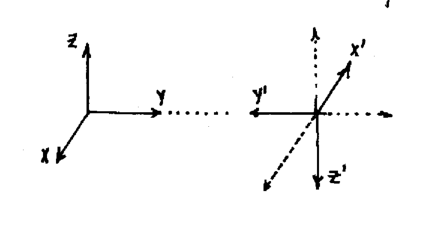
\includegraphics[width=0.6\textwidth]{images/teo2_16.pdf}
	\end{center}
	\caption{}
\end{figure} 
Queremos que refleje el $\Braket{\hat{x}}$ 
\[
	\Braket{\alpha'|\vb{x}|\alpha'} = - \Braket{\alpha|\vb{x}|\alpha} 
\]
\[
	\Braket{\alpha|\Pi^\dagger\vb{x}\Pi|\alpha} = - \Braket{\alpha|\vb{x}|\alpha} \rightarrow
	\Pi^\dagger\vb{x}\Pi = -\vb{x} 
\]
y entonces 
\[
	\{\vb{x},\Pi\} = 0,
\]
anticonmuta con \vb{x}. Debido a ello 
\[
	\Pi\Ket{\vb{x}'} = \Ket{-\vb{x}'} \qquad \Pi^2 \equiv \mathbb{1}
\]
lo cual dice que los autovalores son $\pm 1$ y $\Pi$ es unitario y hermítico.
Como $\hat{\Pi}$ no depende del tiempo 
\[
	\Pi^\dagger\vb{p}\Pi = \Pi^\dagger\dtot{\vb{x}}{t}\Pi = \dtot{}{t}(\Pi^\dagger\vb{p}\Pi) = 
	\dtot{-\vb{x}}{t} \rightarrow \{\vb{p},\Pi\}= 0
\]
y vemos que anticonmuta con \vb{p}.
\vb{x}, \vb{p} son operadores impares. En cambio $\vb{L}=\vb{x}\times\vb{p}$ es un operador par, entonces 
\[
	[\vb{L},\Pi] = 0 \qquad [\vb{J},\Pi] = 0
\]
\begin{figure}[htb]
	\begin{center}
	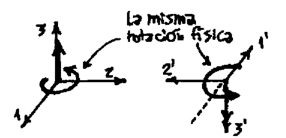
\includegraphics[width=0.6\textwidth]{images/teo2_17.pdf}
	\end{center}
	\caption{}
\end{figure} 
Que conmuta con \vb{J} puede verse de pedirle que 
\[
	[\Pi,\mathcal{D}(R)] = 0 \longrightarrow [\Pi,\vb{J}] = 0 ,
\]
cosa que vale en mecánica clásica, entonces 
\[
	R^{\text{(paridad)}}R^{\text{(rotación)}} = R^{\text{(rotación)}} R^{\text{(paridad)}}
\]
\[
	\Pi^\dagger \Box \Pi =  \begin{cases} +{\Box} \quad \text{par}\quad\text{vector axial( 
	pseudovector)}\\  -\Box \quad \text{impar} \quad \text{vector polar} \end{cases}
\]
\[
	\Pi^\dagger \Box \Pi =  \begin{cases} +\Box \quad \text{par}\quad\text{escalar}\\
	-\Box \quad \text{impar} \quad \text{pseudoescalar} \end{cases}
\]
\[
	\Pi^\dagger \vb{S}\cdot\vb{x} \Pi = \Pi^\dagger \vb{S}\Pi \cdot\Pi^\dagger\vb{x} \Pi =
	\vb{S}\cdot(-\vb{x}) = -\vb{S}\cdot\vb{x}
\]
y $\vb{S}\cdot\vb{x}$ es un pseudoescalar.

\subsection{Función de onda bajo paridad}

\[
	\Psi_\alpha(x') = \Braket{x'|\alpha} = \Braket{x'|\Pi|\alpha} = \Braket{x'|\alpha'} = 
	\Braket{-x'|\alpha}
\]
y entonces la función de onda de un estado al que se le aplicó paridad será 
\[
	\Psi_{\alpha'}(x') = \Psi_\alpha(-x')
\]

Sea $\Ket{\alpha}$ autoestado de paridad, entonces 
\[
	\Pi\Ket{\alpha} = \pm \Ket{\alpha}
\]
los autovalores serán $\pm 1$
\[
	\Braket{x'|\alpha'} = \pm \Braket{x'|\alpha} = \Braket{-x'|\alpha} 
\]
\[
	\Psi_\alpha(-x') = \begin{cases} +\Psi_\alpha(x') \quad \text{función de onda par}\\ 
	-\Psi_\alpha(x') \quad \text{función de onda impar}\\ 
	\end{cases}
\]
no toda función de onda tiene paridad bien definida.

\[
	\vb{x} \to -\vb{x} \longrightarrow \left( r\to r, \theta \to \pi-\theta, \phi \to \phi+\pi \right)
\]
\[
	\Braket{x'|\alpha,\ell,m} = R_\alpha(r) Y_\ell^m(\theta,\phi) \rightarrow \text{con}\vb{x} \; \to 
	-\vb{x} \; \text{será}
\]
\[
	Y_\ell^m(\pi-\theta,\phi+\pi) = (-1)^\ell Y_\ell^m(\theta,\phi)
\]
\[
	\Pi\Ket{\alpha,\ell,m} =  (-1)^\ell \Ket{\alpha,\ell,m}
\]
Como $[\vb{L},\hat{\Pi}]=0$ un autoestado de \vb{L} es autoestado de $\hat{\Pi}$ .

\subsection{Teorema}

Sea $[H,\pi]=0$ y $\Ket{n}$ autoestados no degenerados de $H$ 

	$\Rightarrow$ $\Ket{n}$ es autoestado de $\Pi$.

La demostración 
\[
	\left(\frac{1}{2}\pm \frac{\Pi}{2}\right)\Ket{n} = \frac{\Pi^2\pm\Pi}{2}\Ket{n} = 
	\Pi \left( \frac{\pm 1+\Pi}{2}\right)\Ket{n} = \pm\Pi \frac{1\pm\Pi}{2}\Ket{n}
\]
y entonces es autoestado de paridad con autovalor $\pm 1$. 
\[
	H\frac{1}{2}\left(1\pm\Pi\right)\Ket{n} = \frac{1}{2}E_n\Ket{n} \pm \frac{E_n}{2}\Pi\Ket{n} =
	E_n\left[ \left( \frac{1}{2} \pm \frac{\Pi}{2}\right) \right]
\]
y es autoestado de $H$, de manera que 
\[
	\left( \frac{1\pm\Pi}{2}\right)\Ket{n} = \Ket{n} \Rightarrow \Ket{n} \quad \text{es autoestado de 
paridad}
\]
\[
	\frac{1}{2}\Ket{n} \pm \frac{\Pi}{2}\Ket{n} = \Ket{n}
\]
\[
	\pm \frac{\Pi}{2}\Ket{n} = +\frac{\Ket{n}}{2} \Rightarrow \Pi\Ket{n} = \pm\Ket{n}
\]
Un caso donde falla el teorema 
\[
	[H,\Pi]=0 \quad \text{con} \quad H=\frac{p^2}{2m} 
\]
pero $\Ket{p'}$ no es autoestado de $\Pi$ por la degeneración $\Ket{p'},\Ket{-p'}$ son ambos correspondientes 
al autovalor $p'2/2m$
\[
	\frac{\hat{p}^2}{2m}\Ket{p'} = \frac{{p'}^2}{2m}\Ket{p'} \qquad  \qquad 
	\frac{\hat{p}^2}{2m}\Ket{-p'} = \frac{{p'}^2}{2m}\Ket{-p'}
\]
\[
	\Pi\Ket{p'}= \Ket{-p'}
\]
y $\Ket{p'}$ no es autoestado de $\Pi$.

\subsection{Reglas de selección de paridad $\Pi$}

Sean $\Ket{\alpha}, \Ket{\beta}$ autoestados de paridad 
\[
	\Pi\Ket{\alpha} = \varepsilon_\alpha \Ket{\alpha} \qquad\qquad
	\Pi\Ket{\beta} = \varepsilon_\beta \Ket{\beta}
\]
siendo para el caso impar
\[
	\Braket{\beta|\Box|\alpha} = - \Braket{\beta|\Pi^\dagger\Box\Pi|\alpha} =
	-\varepsilon_\alpha \varepsilon_\beta \Braket{\beta|\Box|\alpha},
\]
y en el caso par
\[
	\Braket{\beta|\Box|\alpha} = \Braket{\beta|\Pi^\dagger\Box\Pi|\alpha} =
	\varepsilon_\alpha \varepsilon_\beta \Braket{\beta|\Box|\alpha}
\]

Si el operador $\Box$ es impar (como $\vb{x}, \vb{p}$) entonces $\varepsilon_\alpha=1,
\varepsilon_\beta=-1$ o bien $\varepsilon_\alpha=-1,\varepsilon_\beta=1$.

Si el operador $\Box$ es par (como $\vb{L}, \vb{S}$) entonces $\varepsilon_\alpha=1,
\varepsilon_\beta=1$ o bien $\varepsilon_\alpha=-1,\varepsilon_\beta=-1$.

\begin{itemize}
 \item Operadores impares solo conectan estados de paridad opuesta
 \item Operadores pares solo conectan estados de la misma paridad 
\end{itemize}

\[
	\Braket{\beta|\vb{x}|\alpha} = 0 
\]
entonces
\[
	\int\int dx'dx''\Braket{\beta|x''}\Braket{x''|\vb{x}|x'}\Braket{x'|\alpha}= 0
\]
y como es $\Braket{x''|\vb{x}|x'} = x' \delta(x' -x'')$
\[
	\int_{-\infty}^{+\infty} dx'\Braket{\beta|x'} x' \Braket{x'|\alpha} =
	\int_{-\infty}^{+\infty} dx'\Psi_\beta^*(x') x' \Psi_\alpha (x')
\]

\section{Inversión temporal (reversión de movimiento)}


En mecánica clásica sería {\it pasar la película hacia atrás}
\[
	t \longrightarrow -t
\]
En sistemas sin fuerzas disipativas se tiene 
\[
	m \ddot{x} = - \dtot{}{x} V(x)
\]
siendo $x(t)$ y $x(-t)$ soluciones de $\vb{F} = m\vb{a}$ pues si $t\to-t$ se tiene
\[
	m \ddot{x} = - \dtot{}{x} V(x)
\]
dado que 
\[
	\dtot[2]{x(t)}{t} = \dtot[2]{x(-t)}{t}
\]

En mecánica cuántica tendremos 
\[
	i \hbar \dpar{\Psi(x,t)}{t} = \left( -\frac{\hbar^2\nabla^2}{2m} + V \right)\Psi(x,t)
\]
y si hacemos el cambio $t\to -t$
\[
	i \hbar \dpar{\Psi(x,-t)}{t} = -i \hbar \dpar{\Psi(x,t)}{t}  = 
	- \left( -\frac{\hbar^2\nabla^2}{2m} + V \right)\Psi(x,t)
\]
se ve que $\Psi(x,-t)$ no es solución de Schrödinger. 

Pero notemos que $\Psi^*(x,-t)$ cumple la ecuación de Schrödinger
\[
	i \hbar \dpar{\Psi^*(x,-t)}{t} = -i \hbar \dpar{\Psi^*(x,t)}{t} 
\]

Entonces necesitamos un operador que respete esta característica.
Necesitaré el producto interno conjugado 
\[
	\Psi_\alpha(x') = \Braket{x'|\alpha} \qquad
	\Psi^*_\alpha(x') = \Braket{x'|\alpha}^* = \Braket{\alpha|x'}
\]
El operador involucrado no será unitario 
\[
	\Ket{\tilde{\alpha}} = \hat{\Theta}\Ket{\alpha} \qquad 
	\Ket{\tilde{\beta}} = \hat{\Theta}\Ket{\beta}
\]
Si $\hat{\Theta}$ unitario se conserva el producto interno 
\[
	\Braket{\hat{\beta}|\hat{\alpha}} = 
	\Braket{\beta|\hat{\Theta}^\dagger\hat{\Theta}|\alpha} =
	\Braket{\beta|\mathbb{1}|\alpha} = \Braket{\beta|\alpha}
\]

Pediremos antiunitariedad y antilinealidad al operador $\hat{\Theta}$
\[
	\Braket{\hat{\beta}|\hat{\alpha}} = \Braket{{\beta}|{\alpha}}^*
\]
\[
	\hat{\Theta}[ C_\alpha\Ket{\alpha} + C_\beta\Ket{\beta}] = 
	C_\alpha^*\hat{\Theta}\Ket{\alpha} + C_\beta^*\hat{\Theta}\Ket{\beta}
\]
siendo lo primero la antiunitariedad y lo segunda la antilinealidad.

Todo operador antiunitario y antilineal puede escribirse como producto 
\[
	\Theta = U K
\]
donde $U$ es unitario y $K$ la conjugación compleja. $K$ no cambia los autoestados, porque en base canónica 
un autoestado tiene un solo elemento (1) que no es nulo.
\[
	K(C\Ket{\alpha}) = CK\Ket{\alpha} = C^*K(\sum_{a'} \Ket{a'}\Braket{a'|\alpha}) =
	C^* (\sum_{a'} \Braket{a'|\alpha}^* K \Ket{a'}) =
	C^* (\sum_{a'} \Braket{a'|\alpha}^* \Ket{a'}) 
\]

Veamos que $UK$ es antiunitario 
\[
	\Ket{\hat{\alpha}} = UK \Ket{\alpha} = \sum_{a'} \Braket{a'|\alpha}^* U\Ket{a'} \qquad \qquad
	\Ket{\hat{\beta}} = UK \Ket{\beta} = \sum_{a''} \Braket{a''|\beta}^* U\Ket{a''}
\]

\[
	\Bra{\hat{\beta}} = \sum_{a''} \Braket{a''|\beta} \Bra{a''}U^\dagger
\]
entonces
\[
	\Braket{\hat{\beta}|\hat{\alpha}} = \sum_{a''} \Braket{a''|\beta} \Bra{a''}U^\dagger
	\sum_{a'} \Braket{a'|\alpha}^* U\Ket{a'}
\]
\[
	\sum_{a',a''} \Braket{a''|\beta} \Braket{a'|\alpha}^* \Bra{a''}U^\dagger U\Ket{a'} =
	\sum_{a'} \Braket{a'|\beta} \Braket{a'|\alpha}^* =  \sum_{a'} \Braket{\beta|a'}^* \Braket{a'|\alpha}^*
	= \Braket{\beta|\alpha}^*
\]
y entonces UK es antinunitario.

Notemos que no se define $\hat{\Theta}^\dagger$ actuando sobre bras. La demostración anterior esperó a 
quitarse de encima $\hat{K}$ para hacer dual conjugado al $\Ket{\tilde{\beta}}$.

\subsection{Operadores ante $\hat{\Theta}$}

Usaremos la notación 
\[
	\Ket{\tilde{\alpha}} = \hat{\Theta} \Ket{\alpha}
\]
donde hay que tener en cuenta 
\[
	\Theta^\dagger \Theta = \mathbb{1}
\]
pues $\Theta^\dagger$ no está definido.

Sería razonable esperar que 
\[
	\Braket{\hat{\alpha}|\vb{p}|\hat{\alpha}} = - \Braket{{\alpha}|\vb{p}|{\alpha}}\qquad 
	\Braket{\hat{\alpha}|\vb{x}|\hat{\alpha}} = \Braket{{\alpha}|\vb{x}|{\alpha}}\qquad 
\]
Sea $\hat{\mathbb{O}}$ un operador hermítico 
\[
	\Braket{\alpha|\mathbb{O}|\alpha} = \Braket{\alpha|\gamma}
\]
\[
	\Braket{\hat{\alpha}|\hat{\gamma}}^* = \Braket{\alpha|\gamma} \Rightarrow 
	\Braket{\hat{\alpha}|\hat{\gamma}} = \Braket{\gamma|\alpha}
\]
y como $\Braket{\hat{\alpha}|\Theta|\gamma} = \Braket{\hat{\alpha}|\Theta\mathbb{O}|\alpha}$.
Luego metemos un $\Theta^{-1}\Theta = 1$
\[
	\Braket{\hat{\alpha}|\Theta\mathbb{O}\Theta^{-1}\Theta|\alpha} =
	\Braket{\hat{\alpha}|\Theta\mathbb{O}\Theta^{-1}|\hat{\alpha}} = \Braket{\alpha|\mathbb{O}|\alpha}
\]

Notamos que no se aplica $\Theta$ sobre bra alguno y tenemos $\Theta$ no unitario. Entonces requeriremos 
\[
	\Theta \hat{p} \Theta^{-1} = -\hat{p} \qquad \Theta \hat{j} \Theta^{-1} = -\hat{j}
\]
\[
	\hat{\Theta}\hat{p} = -\hat{p}\hat{\Theta} \quad \Rightarrow 
	\quad \{ \hat{\Theta},\hat{p}\} = 0
\]
como para $\vb{p},\vb{J}$ operadores impares 
\[
	\Theta \hat{x} \Theta^{-1} = \hat{x}
\]
\[
	\hat{\Theta}\hat{x} = -\hat{x}\hat{\Theta} \quad \Rightarrow 
	\quad [ \hat{\Theta},\hat{x} ] = 0
\]
y $\vb{x}$ operador par.

Los operadores pares conmutan con $\Theta$,
\[
	= =
\]
\begin{figure}[htb]
	\begin{center}
	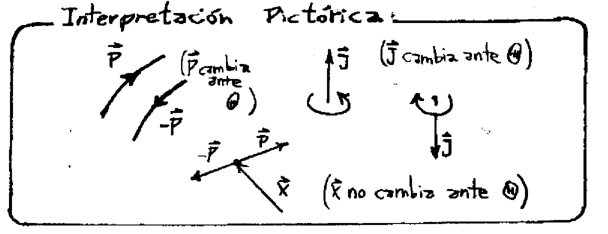
\includegraphics[width=0.6\textwidth]{images/teo2_18.pdf}
	\end{center}
	\caption{}
\end{figure} 
Hamiltoniano ante reversión de movimiento. Veamos la reversión de un sistema en estado $\Ket{\alpha}$
\[
	=
\]
Si el hamiltoniano es invariante ante reversión temporal debería ser lo mismo 
\[
	=
\]
es decir que estamos pidiendo que se obtenga el mismo estado 
\begin{itemize}
 \item Si revertimos el movimiento y evolucionamos $\delta t$.
 \item Si evolucionamos hacia atrás $-\delta t$ y revertimos el movimiento.
\end{itemize}
\begin{figure}[htb]
	\begin{center}
	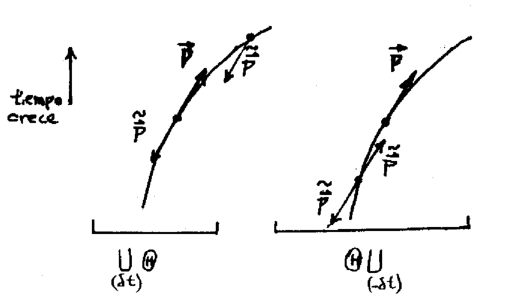
\includegraphics[width=0.6\textwidth]{images/teo2_19.pdf}
	\end{center}
	\caption{}
\end{figure} 
Veamos que vale lo anterior, pensando que si vale se tiene 
\[
	=
\]
\[
	=  \qquad [H,\Theta]=0
\]

Si $\Theta$ era unitario teníamos la relación de anticonmutación $\{ H, \Theta \}=0$ lo cual lleva a absurdos.
\[
	a
\]
Si $\{ H,\Theta \} = 0$
\[
	= \text{H debe ser par frente a $\Theta$}
\]

\subsection{Función de onda}

Sea en $t=0$ un sistema en el estado $\Ket{\alpha}$
\[
	= = 
\]
\[
	\Psi
\]
Esto era lo que {\it vimos} en la ecuación de Schrödinger.

\subsection{Reversión de movimiento sobre \vb{J}}


no tiene sentido porque $J_x,J_y,J_z$ no conmutan entre ellos. Analizaremos $\Ket{\ell,m}$
\[
	\Theta \Ket{\vb{J}} 
\]
\[
	\equiv 
\]

Lo que hace $\Theta$ es invertir la componente de $\hat{z}$ y alterar la fase. Se ve que 
\[
	\Theta^2 = \mathbb{1}
\]

\subsection{Reversión para sistemas de spin $1/2$}

Sea un estado general up de spin $\Ket{\hat{n};+}$, que se obtiene con dos rotaciones 
\[
	Sn
\]
\[
	\Theta
\]
\[
	a
\]
\[
	b
\]
\[
	c
\]

\subsection{Teorema}

Sea $H$ invariante ante $\Theta$ y los $\Ket{n}$ no degenerados, entonces la autofunción de energía puede 
hacerse real tomando una fase apropiada.

Demostración 
\[
	H \Theta  \Ket{n} =
\]
\[
	=
\]
\[
	=
\]

Si le aplico al sistema transformaciones dadas por operadores que conmutan con el H no lo sacamos del 
autoestado en que se encuentra con el paso del tiempo.
En ese sistema solo será razonable medir variables representadas por esos operadores; puesto que de lo 
contrario estamos alterando el sistema y nos es imposible saber donde ha quedado.



% \bibliographystyle{CBFT-apa-good}	% (uses file "apa-good.bst")
% \bibliography{CBFT.Referencias} % La base de datos bibliográfica

\end{document}

	
		\documentclass[10pt,oneside]{CBFT_book}
	% Algunos paquetes
	\usepackage{amssymb}
	\usepackage{amsmath}
	\usepackage{graphicx}
	\usepackage{libertine}
	\usepackage[bold-style=TeX]{unicode-math}
	\usepackage{lipsum}

	\usepackage{natbib}
	\setcitestyle{square}

	\usepackage{polyglossia}
	\setdefaultlanguage{spanish}
	



	\usepackage{CBFT.estilo} % Cargo la hoja de estilo

	% Tipografías
	% \setromanfont[Mapping=tex-text]{Linux Libertine O}
	% \setsansfont[Mapping=tex-text]{DejaVu Sans}
	% \setmonofont[Mapping=tex-text]{DejaVu Sans Mono}

	%===================================================================
	%	DOCUMENTO PROPIAMENTE DICHO
	%===================================================================

\begin{document}

% =================================================================================================
\chapter{Métodos perturbativos}
% =================================================================================================

Se basan en 
\[
	H = H_0 + \lambda V \qquad \lambda \ll 1
\]
con $ H_0\Ket{n^{(0)}} = E_n^{(0)}\Ket{n^{(0)}}$ (el problema sin perturbar)
\[
	H
\]
que sería la solución exacta.
Como esto es hartocomplicado podemos desarrollar en serie 
\[
	\approx 
\]
\[
	\approx 
\]
\[
	()[] = ()()
\]
\[
	\sum_{i=0}^\infty =
\]
y aproximando los primeros términos 
\[
	H_0
\]
\[
	E_0
\]
ahora igualamos orden a orden y resulta 
\[
	\lambda^0 ....
\]
\[
	\lambda^1 ....
\]
\[
	\lambda^2 ....
\]

Pediremos una normalización a cada orden y considerando $ \Braket{0_n|n(\lambda)} \in \mathbb{R}$
\[
	()() =
\]
\[
	\lambda
\]
\[
	...
\]
\[
	...
\]

En un mismo autoestado $(n)$ los órdenes diferentes $(i)$ no son necesariamente ortogonales.

\section{Resolución}

A orden cero será 
\[
	() \qquad \text{y se define} \qquad 
\]
y $\Ket{0_n}$ es dato porque es el estado no perturbado.
A orden uno tenemos 
\[
	()
\]
\[
	\Braket{}
\]
y la energía a orden uno es 
\[
	=
\]

Veamos el autoestado a orden uno. Podemos poner (no hay degeneración)
\[
	=
\]
y sea $p\neq n$
\[
	+ = 0
\]
\[
	=
\]
a un mismo orden (cero) diferentes autoestados son ortogonales.
Sea $p=n$ entonces 
\[
	= 0 
\]
ya lo vimos antes, en la normalización
\[
	=
\]
autoestado hasta orden uno. A orden dos tenemos 
\[
	+ - = 0
\]
\[
	+ - = 0
\]
\[
	=
\]
\[
	E
\]
que es la energía a orden dos.
Veamos el autoestado a orden dos 
\[
	\Ket{2n} = \sum_p ()\Ket{\phi_p}
\]
sea $p\neq n$ 
\[
	+
\]
\[
	+
\]
\[
	=
\]
\[
	+
\]
\[
	+
\]

Sea $p=n$
\[
	+ = 1
\]
\[
	=
\]
\[
	=
\]

\[
	\Ket{2n} =
\]
y el autoestado hasta orden dos
\[
	=
\]
con la energía hasta orden dos 
\[
	=
\]

\subsection{Caso degenerado}

Sea que hay degeneración de orden $g$ en el autoestado $N$( a orden cero)
\[
	= k=1,2,...,g
\]
Suponemos existe combinación lineal 
\[
	+
\]
para escribir un estado degenerado en función de los otros.
\[
	= 0
\]
\[
	= 0
\]
\[
	=0
\]
\[
	=0
\]
\[
	=
\]
Esto último es una ecuación de autovalores y autovectores de la forma:
\[
	= 0 
\]
nos dará los corrimientos de la energía a primer orden  y los autoestados $\Ket{1_n^j}$ serán los 
autovectores del problema.

\section{Efecto Stark}

Sea un átomo de H con $\Ket{n,\ell,m}$ sin spín y con $n=2$. Será 
\[
	0
\]
Tengo cuatro estados 
\[
	2 0 0 
\]
todos con la misma energía $\epsilon_2$.
Metemos un campo eléctrico en $\hat{z}$ y entonces $V=-ez|\vb{E}|$. Luego 
\[
	=
\]
$\hat{z}$ es impar ante paridad y entonces vincula estados de paridad diferente,
y entonces 
\[
	= 0 
\]
diagonal nula y con $m'\neq m$ a igual $\ell$ tiene la misma paridad
\[
	=
\]

Solo hay un elemento no nulo correspondiente al producto par-impar.
Se tendrá 
\[
	=
\]
Puedo diagonalizar y obtengo 
\[
	=
\]

En este caso no se rompe la degeneración por completo.
\[
	=
\]
\begin{figure}[htb]
	\begin{center}
	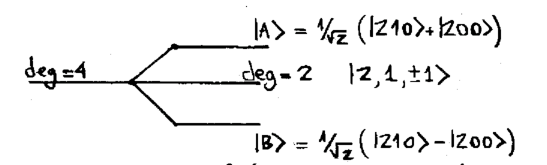
\includegraphics[width=0.6\textwidth]{images/teo2_20.pdf}
	\end{center}
	\caption{}
\end{figure} 

\subsection{Corrimiento de la energía a orden 2 (con degeneración)}

Sea que a orden uno se rompe toda la degeneración 
\[
	+ - = 0
\]
Entonces la corrección a segundo orden de la energía será:
\[
	+ - = E
\]
pues $\Braket{0_N^j|0_N^j}= 0$ pero 
\[
	=
\]
\[
	=
\]
falta desarrollo ...

\[
	E =
\]
donde $N$ es un estado degenerado.

\section{Estructura fina del átomo de hidrógeno}

La solución tradicional del átomo de H usa el potencial coulombiano. Esto desemboca en las funciones 
$\Ket{n,\ell,m}$, sin embargo la introducción de ajuste como {\it perturbaciones} rompe algo la degeneración.
\[
	cuentitas
\]
donde $a_0$ es el radio de Bohr, $\alpha$ es la constante de estructura fina .
Tenemos 
a) Corrección cinemática (relativista)
\[	
	0
\]
y esta corrección va como $W_{mv}/H_0 \sim \alpha^2$.

b) Acoplamiento spín-órbita
Se puede pensar considerando un $e^-$ en reposo con un protón orbitando que genera un $\vb{B}_{eff}$
\[
	W_{so} =
\]
y la corrección va como $W_{mv}/H_0 \approx \alpha^2$.

c) Término de Darwin o de contacto
\[
	=
\]
que va como  $W_{D}/H_0 \approx \alpha^2$.

Hay otras correcciones hiperfinas que provienen del spín del electrón y del spín del protón. Pero van como 
$\alpha^2/2000$.
Si consideramos el sistema con 
\[
	n=2
\]
serán ocho estados.
\[
	W
\]
y W es par ante $\Pi$ y sólo habrá elementos de matriz $\neq 0$ que sean de la misma paridad.
\[
	matriz
\]
y entonces $\Ket{2s}, \Ket{2p}$ no están conectados.

De manera que hay ocho estados $\Ket{n=2,\ell,m_\ell,s,m_s}$ que al calcular esta perturbación W resultan 
\begin{figure}[htb]
	\begin{center}
	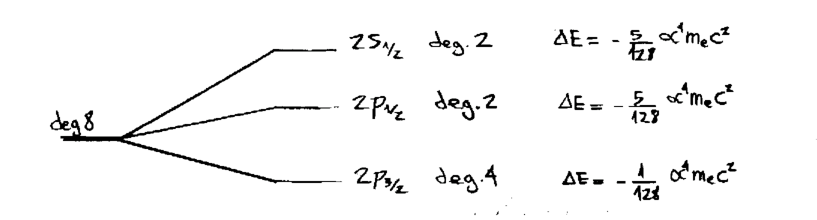
\includegraphics[width=0.9\textwidth]{images/teo2_21.pdf}
	\end{center}
	\caption{}
\end{figure} 
\[
	dg
\]
El cálculo para las correcciones hiperfinas no condice la experiencia. Se necesita aquí mecánica cuántica 
relativista. Los dos primeros niveles tienen la misma $\Delta E$ porque en MCR se ve que 
\[
	E = 
\]
es decir que no depende directamente de $\ell,s$.

Un sketch de los métodos perturbativos
\[
	H_0 = 
\]



% \bibliographystyle{CBFT-apa-good}	% (uses file "apa-good.bst")
% \bibliography{CBFT.Referencias} % La base de datos bibliográfica

\end{document}

	
%  		\documentclass[10pt,oneside]{CBFT_book}
	% Algunos paquetes
	\usepackage{amssymb}
	\usepackage{amsmath}
	\usepackage{graphicx}
	\usepackage{libertine}
	\usepackage[bold-style=TeX]{unicode-math}
	\usepackage{lipsum}

	\usepackage{natbib}
	\setcitestyle{square}

	\usepackage{polyglossia}
	\setdefaultlanguage{spanish}
	



	\usepackage{CBFT.estilo} % Cargo la hoja de estilo

	% Tipografías
	% \setromanfont[Mapping=tex-text]{Linux Libertine O}
	% \setsansfont[Mapping=tex-text]{DejaVu Sans}
	% \setmonofont[Mapping=tex-text]{DejaVu Sans Mono}

	%===================================================================
	%	DOCUMENTO PROPIAMENTE DICHO
	%===================================================================

\begin{document}

% =================================================================================================
\chapter{Conceptos fundamentales de electromagnetismo}
% =================================================================================================


% =================================================================================================
\section{Ecuaciones de Maxwell}
% =================================================================================================

Son ecuaciones lineales de modo que vale la superposición (con \vb{E}, \vb{B} y 
cualquier vector relacionado linealmente con ellos).
\[
	\nabla \cdot \vb{D} = 4 \pi \rho_\ell \qquad \nabla \cdot \vb{B} = 0
\]
\[
	\nabla \times \vb{E} = - \frac{1}{c} \dpar{B}{t} \qquad \nabla \times \vb{H} =
	\frac{4\pi}{c} \vb{J}_\ell + \frac{1}{c}\dpar{D}{t}
\]
\[
	\vb{F} = q \left( \vb{E} + \frac{1}{c} \vb{v} \times \vb{B} \right)
\]

Los vectores pueden ser polares (tienen físicamente bien definido el sentido) o
axiales (se les atribuye un sentido por convención).

Las ecuaciones son invariantes ante transformaciones del tipo: rotación
y reflexión espacial y temporal.

% =================================================================================================
\section{Electrostática}
% =================================================================================================

La ley de Coulomb reza que
\[
	\vb{F}_{12} = q_1 q_2 \frac{(\vb{x}_1 - \vb{x}_2)}{|\vb{x}_1 - \vb{x}_2 |^3}
\]
que es la fuerza sobre 1 debido a 2. De la ley de Coulomb se puede definir 
\[
	\vb{E}_{12}(\vb{x}_1) \equiv \vb{F}_{12}/q_1
\]
y tomando $\vb{x}_1 \equiv \vb{x}$ y haciendo el límite $q_1 \to 0$ se tiene
\[
	\vb{E}(\vb{x}) = \sum_{i=1}^N \; q_i \frac{(\vb{x} - \vb{x}_i)}{|\vb{x} - \vb{x}_i |^3}
\]
que es el campo eléctrico y que en el paso al continuo resulta
\[
	\vb{E}(\vb{x}) = \int_{V'} \rho(\vb{x}) \frac{(\vb{x} - \vb{x}_i)}{|\vb{x} - \vb{x}_i |^3} dV' 
\]
siendo \vb{x} punto campo y $\vb{x}_i$ punto fuente.

\begin{figure}[htb]
	\begin{center}
	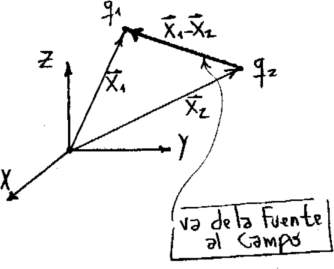
\includegraphics[width=0.6\textwidth]{images/fig_ft1_ejescargas.pdf}	 
	\end{center}
	\caption{}
\end{figure} 

\subsection{Conservación de la carga}

La carga total sale de una integral 
\[
	Q = \int_{V'}  \rho(\vb{x}') dV'
\]
como muestra la imagen
\begin{figure}[htb]
	\begin{center}
	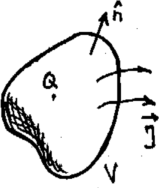
\includegraphics[width=0.25\textwidth]{images/fig_ft1_conserv.pdf}	 
	\end{center}
	\caption{}
\end{figure} 
y si el volumen es fijo podemos tomar la derivada con respecto al tiempo que pasa el interior como
derivada parcial,
\[
	\dtot{Q}{t} = \int_{V'} \dpar{\rho}{t} (\vb{x}') dV' = - \int_{S\equiv\partial V'} \vb{J} \cdot d\vb{S}
\]
y el miembro extremo derecho  se debe a que si la carga varía es a consecuencia de que se va en
forma de flujo. Aplicando el teorema de la divergencia en el miembro derecho,
\[
	\int_{V'} \dpar{\rho}{t} (\vb{x}') dV' = - \int_{V'} \nabla \cdot \vb{J} \; dV'
\]
lo cual vale para todo volumen y entonces esto significa que
\[
	\dpar{\rho}{t} + \nabla \cdot \vb{J} = 0
\]
que es la ecuación de continuidad de la carga. Si fuera $\nabla \cdot \vb{J}=0$ esto significa que las líneas
de \vb{J} no tienen principio ni fin.

% =================================================================================================
\section{Interacción magnética}
% =================================================================================================

Cuando se da $\nabla \cdot \vb{J}=0$ hablamos de una corriente estacionaria (no hay acumulación de carga en
ninguna parte). Las corrientes estacionarias producen efectos magnéticos dados por la ley de Biot-Savart
\[
	\vb{B}(\vb{x}) = \frac{1}{c} \int_\Gamma \frac{I d\vb{\ell}' \times (\vb{x} - \vb{x}')}{|\vb{x} - \vb{x}'|^3} 
\]
que es válida para un circuito $\Gamma$, que es una curva que se recorre en sentido CCW.
En el caso de un volumen la expresión es 
\[
	\vb{B}(\vb{x}) = \frac{1}{c} \int_{V'} \frac{ \vb{J}(\vb{x}') \times (\vb{x} - \vb{x}')}{|\vb{x} - \vb{x}'|^3} 
dV'
\]
mientras que la fuerza sobre un circuito $\Gamma$ es
\[
	F = \frac{1}{c} \int_\Gamma I d\vb{\ell} \times \vb{B}
\]
y sobre un volumen 
\[
	F = \frac{1}{c} \int_V \vb{J} \times \vb{B} dV
\]

La transformación entre estas integrales puede hacerse merced al siguiente razonamiento,
% \begin{align*}
%  	I d\vb{\ell} \times \vb{B} = \vb{J}  \cdot d\vb{S} d\vb{\ell}  \times \vb{B} =
%   	\cos(\theta) dS \vb{J} d\ell \times \vb{B} = \\
% 	\vb{J} \times \vb{B}  \cos(\theta) dS d\ell  = \vb{J} \times \vb{B}  d\vb{S} \cdot d\vb{\ell}  = 
% 	\vb{J} \times \vb{B}  dV 
% \end{align*}
\[
  	I d\vb{\ell} \times \vb{B} = \vb{J}  \cdot d\vb{S} d\vb{\ell}  \times \vb{B} =
  	\cos(\theta) dS \vb{J} d\ell \times \vb{B} = 
\]
\[
	\vb{J} \times \vb{B}  \cos(\theta) dS d\ell  = \vb{J} \times \vb{B}  d\vb{S} \cdot d\vb{\ell}  = 
	\vb{J} \times \vb{B}  dV 
\]

\subsection{Fuerza de un circuito sobre otro}

La fuerza de un circuito 2 sobre otro circuito 1 puede calcularse con un poco de paciencia como sigue
\[
	F_{12} = \frac{1}{c} \int_{\Gamma_1} I_1 d\vb{\ell}_1 \times \left\{
	\frac{1}{c} \int_{\Gamma_2} \frac{I_2 d\vb{\ell}_2 \times (\vb{x}_1 - \vb{x}_2)}{|\vb{x}_1 - \vb{x}_2|^3} 
	\right\}
\]
\[
	F_{12} = \frac{I_1 I_2}{c^2} \int_{\Gamma_1} \int_{\Gamma_2} d\vb{\ell}_1 \times \left\{
	\frac{d\vb{\ell}_2 \times (\vb{x}_1 - \vb{x}_2)}{|\vb{x}_1 - \vb{x}_2|^3} 
	\right\}
\]
\[
	F_{12} = \frac{I_1 I_2}{c^2} \int_{\Gamma_1} \int_{\Gamma_2} d\vb{\ell}_2  \left\{
	\frac{d\vb{\ell}_1 \cdot (\vb{x}_1 - \vb{x}_2)}{|\vb{x}_1 - \vb{x}_2|^3} 
	\right\} - \int_{\Gamma_1} \int_{\Gamma_2} \frac{ (\vb{x}_1 - \vb{x}_2)}{|\vb{x}_1 - \vb{x}_2|^3} 
	\left\{ d\vb{\ell}_1 \cdot d\vb{\ell}_2 \right\}
\]
donde el primer término se comprueba nulo si se reescribe utilizando que
\[
	\frac{ (\vb{x}_1 - \vb{x}_2)}{|\vb{x}_1 - \vb{x}_2|^3} = 
	\nabla_{\vb{x}_2} \frac{ 1 }{|\vb{x}_1 - \vb{x}_2|} =
	- \nabla_{\vb{x}_1} \frac{ 1 }{|\vb{x}_1 - \vb{x}_2|} 
\]
de manera que entonces
\[
	- \int_{\Gamma_2} d\vb{\ell}_2  \int_{\Gamma_1} d\vb{\ell}_1 \cdot \nabla_{\vb{x}_1} \frac{ 1 }{|\vb{x}_1 - \vb{x}_2|} 
\]
donde se ve que es nula la última integral dado que 
\[
	\int_{\Gamma_1} d\vb{\ell}_1 \cdot \nabla_{\vb{x}_1} = 0.
\]

Entonces, se tiene 
\[
	F_{12} = - \frac{I_1 I_2}{c^2} \int_{\Gamma_1} \int_{\Gamma_2} \frac{ (\vb{x}_1 - \vb{x}_2)}{|\vb{x}_1 - \vb{x}_2|^3} 
	\left( d\vb{\ell}_1 \cdot d\vb{\ell}_2 \right)
\]
que vale lo mismo si intercambiamos $\Gamma_1$ con $\Gamma_2$ en la integración. Podemos decir que con corrientes estacionarias
vale el principio de acción y reacción: las fuerzas son iguales y de sentido opuesto.


% =================================================================================================
\section{Teorema de Helmholtz}
% =================================================================================================

Nos dice que un campo vectorial está completamente determinado por su divergencia y su rotor.
Por ejemplo, para un campo eléctrico 
\[
	\vb{E} = \int_{V'} \rho \frac{\vb{x} - \vb{x}'}{|\vb{x} - \vb{x}'|^3} dV' = 
		- \int_{V'} \rho \nabla_{\vb{x}} \frac{ 1 }{|\vb{x} - \vb{x}'|} dV' = 
		- \nabla_{\vb{x}} \int_{V'}   \frac{ \rho }{|\vb{x} - \vb{x}'|} dV' = 
\]
y esta última es la integral de Poisson
\[
	\vb{E} = - \nabla_{\vb{x}} \phi (\vb{x}).
\]
Entonces $\vb{E}$ es un gradiente y por ello 
\[
	\nabla  \times \vb{E} = 0
\]
de manera que $\vb{E}$ es conservativo, cumple $\int \vb{E}\cdot d\vb{\ell} = 0$ o lo que
es lo mismo, $\vb{E}$ es irrotacional.
Hemos hecho la construcción de un potencial electrostático.

% =================================================================================================
\section{Ley de Gauss}
% =================================================================================================



\begin{figure}[htb]
	\begin{center}
	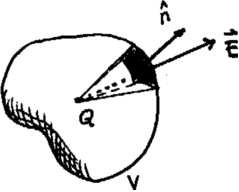
\includegraphics[width=0.35\textwidth]{images/fig_ft1_gauss.pdf}	 
	\end{center}
	\caption{}
\end{figure} 
\[
	\vb{E} \cdot \hat{n} = q \frac{\cos(\theta)}{r^2}
\]
y el ángulo sólido es
\[
	\vb{E} \cdot \hat{n} dS = q \frac{\cos(\theta)}{r^2} dS
\]
\[
	\vb{E} \cdot \hat{n} dS = q d\Omega \qquad \longrightarrow \qquad 
	\int_{S\equiv\partial V} \vb{E} \cdot \hat{n} \; dS = q \int_S d\Omega =
	\begin{cases}
	 0 \quad \textrm{carga exterior}\\
	 4\pi \quad \textrm{carga interior}
	\end{cases}
\]
\[
	\int_S \vb{E} \cdot \hat{n} \; dS = 4\pi \sum_i q_i
\]
La ley de Gauss es
\[
	\int_S \vb{E} \cdot \hat{n} \; dS = 4\pi Q_n
\]
donde $Q_n$ es la carga neta dentro de la superficie $S$. Al continuo pasa como 
\[
	\int_S \vb{E} \cdot \hat{n} \; dS = 4\pi \int_V \rho \: dV
\]
de manera que 
\[
	\int_V \divem{E} \; dV = \int_V 4\pi \rho \: dV
\]
y entonces
\[
	\divem{E} = 4\pi \rho.
\]

Por otro lado si \vb{E} es el gradiente de un potencial $\phi$ se tiene
\[
	\divem{E} = \Nabla\cdot{(-\Nabla\phi)} = - \lapm\phi = 4\pi \rho
\]
y se desprenden las ecuaciones de Poisson,
\[
	\lapm\phi = -4\pi \rho
\]
y de Laplace
\[
	\lapm\phi = 0
\]
que es el caso particular de la anterior con cargas nulas.

La solución de la ecuación no homogénea es suma de una solución del homogéneo más una solución
particular. La carga está relacionada a la solución particular.

\subsection{Gauges}

Dado que $\divem{B}=0$ entonces existe un \vb{A} tal que 
\[
	\rotorm{A} = \vb{B}
\]
pero para caracterizar totalmente el \vb{A} tengo la libertad de definir a conveniencia
\[
	\divem{A} \equiv \; \textrm{``el gauge''}.
\]
Casos particulares importantes son el gauge de Coulomb,
\[
	\divem{A} = 0
\]
de manera que como 
\[
	\Nabla \times (\rotorm{A}) = \Nabla(\divem{A}) - \lapm{\vb{A}} = \frac{4\pi}{c}\vb{J}
\]
se llega para el potencial electromagnético, bajo el gauge de Coulomb, a que 
\[
	\lapm{\vb{A}} = - \frac{4\pi}{c}\vb{J} 
\]

	\begin{table}[hbt]
	\centering
        \begin{tabular}{|c|c|}
		\hline
		& \\
		$\displaystyle{\vb{E} = \int_{V'} \frac{\rho(\vb{x}')(\vb{x}-\vb{x}')}{|\vb{x}-\vb{x}'|^3} dV' 
		}$ & $\displaystyle{\vb{B} = \frac{1}{c} \int_{V'} \frac{\vb{J}(\vb{x}') \times 
		(\vb{x}-\vb{x}')}{|\vb{x}-\vb{x}'|^3} dV'}$ \\
		& \\
		\hline
		Ley de Gauss & Ley de Ampere \\
		& \\
		$\displaystyle{\int_S \vb{E}\cdot d\vb{S} = 4\pi Q_n}$ &
		$\displaystyle{\int_\Gamma \vb{B}\cdot d\vb{\ell} = \frac{4\pi}{c} I_c}$ \\
		& \\
		\hline
		&\\
		$\divem{E} = 4\pi\rho$ & $\divem{B} = 0$ \\
		$\rotorm{E} = 0$ & $\rotorm{B} = \frac{4\pi}{c}\vb{J}$ \\
		& \\
		\hline
		& \\
		$\vb{E} = - \Nabla\phi$ & $\vb{B} = \rotorm{A}$ \\
		& \\
		\hline
        \end{tabular} 
	\caption{}
	\end{table} 

La operación de tomar rotor y el producto vecrtorial cambian el carácter de los vectores: de
polares pasan a axiales y viceversa.

La fuerza general sobre una distribución de carga es
\[
	\vb{F} = \int_{V'} \rho \vb{E} dV' + \frac{1}{c} \int_{V'} \vb{J} \times \vb{B} dV'. 
\]

\subsection{Delta de Dirac}

Una densidad de carga puntual se puede escribir mediante una delta de Dirac de acuerdo a
\[
	\rho(\vb{x}') = q\: \delta (\vb{x} - \vb{x}') = \begin{cases}
	                                               0 \qquad \vb{x} \neq \vb{x}' \\
	                                               \infty \qquad \vb{x} = \vb{x}'\\
	                                              \end{cases}
\]
siendo las dimensiones de la delta las de $1/L^3$ y cumpliéndose 
\[
	\int_{V'} \delta (\vb{x} - \vb{x}') dV' = 1
\]
\[
	\delta (\vb{x} - \vb{x}') = \frac{1}{h_1h_2h_3} \delta(q_1-q_1') \delta(q_2-q_2') \delta(q_3-q_3')
\]
donde $q_1, q_2$ y $q_3$ son coordenadas curvilíneas generales y $h_1h_2h_3$ es el jacobiano
de la transformación.
Luego
\[
	\int f(\vb{x}) \delta' (\vb{x} - \vb{x}_0) dx = -f'(\vb{x}_0)
\]



\subsection{reflexión}

Un vector polar sufre reflexión especular mientras que un vector axial ({\it pseudovector})
sufre una antireflexión especular. Ver la figura.

\begin{figure}[htb]
	\begin{center}
	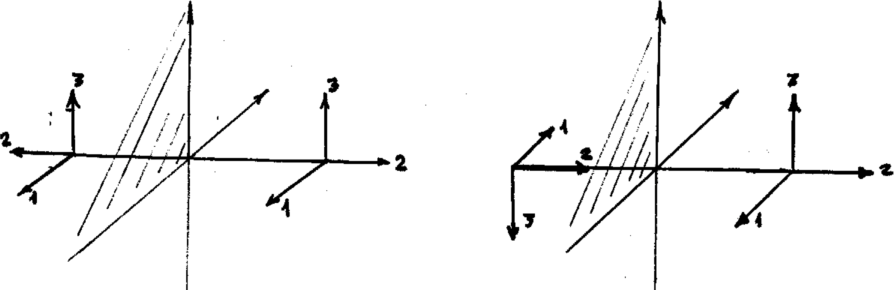
\includegraphics[width=0.6\textwidth]{images/fig_ft1_reflexvect.pdf}	 
	\end{center}
	\caption{}
\end{figure} 

Una reflexión más una rotación permite eliminar componentes de campo.
Una simetría más una rotación-traslación permite eliminar dependencias.

Lo primero que debe hacerse es escribir bien la \vb{J} a partir del dato de la corriente
(que es el que se suele tener) mediante
\[
	i = \int_S \vb{J} \cdot d \vb{S}
\]
En cambio, para \vb{A} es más fácil usar
\[
	\vb{B} = \rotorm{A}
\]
y despejar de aquí la ecuación diferencial que emplear
\[
	\vb{A} = \frac{1}{c} \int_V \frac{\vb{J}}{|\vb{x}-\vb{x}'|} dV
\]


\section{El potencial vector}

Por la ley de Biot y Savart,
\[
	\vb{B} = \frac{1}{c} \int_{V'} \frac{\vb{J}(\vb{x}') \times (\vb{x}-\vb{x}')}{|\vb{x}-\vb{x}'|^3} 
	dV' = \Nabla_x \times \frac{1}{c} \int_{V'} \frac{\vb{J}(\vb{x}')}{|\vb{x}-\vb{x}'|} dV'
\]
de modo que
\be
	\vb{A} = \frac{1}{c} \int_{V'} \frac{\vb{J}(\vb{x}')}{|\vb{x}-\vb{x}'|} dV'
	\label{potvec}
\ee
pero 
\[
	\vb{A}' \equiv \vb{A} + \Nabla \Psi
\]
es tan buen potencial vector como \vb{A} puesto que los rotores verifican $\rotorm{A}=\rotorm{A}'=\vb{B}$,
de lo cual extraemos en conclusión que el potencial vector está definido a menos del gradiente de una
función escalar.

Tomándole el rotor a \eqref{potvec} y considerando $\Nabla'\cdot\vb{J}(\vb{x}')=0$ lo cual se verifica si
la corriente es estacionaria se tiene 
\[
	\rotorm{B} = \frac{4\pi}{c} \vb{J}(\vb{x})
\]
y entonces
\[
	\int_S \rotorm{B} \cdot d\vb{S} = \frac{4\pi}{c} \int_S \vb{J}(\vb{x}) \cdot d\vb{S}
\]
y por el teorema de Stokes arribamos a
\[
	\int_{\Gamma\equiv\partial S} \vb{B}\cdot d\vb{\ell} = \frac{4\pi}{c} I_\Gamma
\]
que es la ley de Ampere. Notemos que $I_\Gamma$ es la corriente concatenada por el lazo $\Gamma$.
Además
\[
	\rotorm{B} = \Nabla\times(\rotorm{A}) = \Nabla(\divem{A}) - \nabla^2 \vb{A} = \frac{4\pi}{c}\vb{J}
\]
pero utilizando el gauge de Coulomb es $\divem{A}=0$ y entonces
\[
	\nabla^2 \vb{A} = -\frac{4\pi}{c}\vb{J}
\]
que es una ecuación de Poisson vectorial.

Magnetostática y electrostáctica son gobernadas por ecuaciones de Poisson para potenciales $\vb{A},\phi$ y
el problema entonces se reduce a resolverlas para luego hallar los campos por derivación.

\section{Unicidad de problemas de potencial}

Si dos problemas satisfacen iguales condiciones de contorno entonces en el recinto encerrado por
ese contorno tienen igual solución.

Si en un recinto $R$
\be
	\phi_1|_{cont} = \phi_2|_{cont}
	\label{potnounico}
\ee
pero se da para el interior de $R$ que $\phi_1\neq\phi_2$ entonces se tiene sucesivamente
\[
	U \equiv \phi_1 - \phi_2 \qquad \qquad \Nabla U = \Nabla \phi_1 - \Nabla \phi_2
\]
\[
	\lapm{U} = \lapm{\phi_1} - \lapm{\phi_2} = -4\pi \rho + 4\pi\rho = 0
\]
\[
	\Nabla\cdot\left( U\Nabla U \right) = U\left( \Nabla\cdot\Nabla U \right) + \Nabla U \cdot \Nabla U
\]
\[
	\int_V \Nabla\cdot\left( U\Nabla U \right) dV = \int_V U \lapm{U}  + (\lapm{U})^2 dV =  \int_V (\lapm{U})^2 dV
\]
llegando al último miembro porque el potencial $U$ cumple la ecuación de Laplace. Luego,
\[
	\int_V (\lapm{U})^2 dV = \int_S U\Nabla{U} \cdot d\vb{S} = 0
\]
habiéndose pasado a la integral de superficie por el teorema de la divergencia y anulando el valor global porque 
$U$ en el contorno es nula (recuérdese \eqref{potnounico}). Además, 
\[
	\Nabla{U} \cdot d\vb{S}  \longrightarrow \left.\dpar{U}{\hat{n}}\right|_{cont}
\]
luego,
\[
	\Nabla U = 0 \qquad \Nabla\phi_1 = \Nabla\phi_2 
\]
y entonces
\[
	\phi_1 = \phi_2 .
\]
a menos, por supuesto, de una constante.



% \bibliographystyle{CBFT-apa-good}	% (uses file "apa-good.bst")
% \bibliography{CBFT.Referencias} % La base de datos bibliográfica

\end{document}

	
%  		\documentclass[10pt,oneside]{CBFT_book}
	% Algunos paquetes
	\usepackage{amssymb}
	\usepackage{amsmath}
	\usepackage{graphicx}
	\usepackage{libertine}
	\usepackage[bold-style=TeX]{unicode-math}
	\usepackage{lipsum}

	\usepackage{natbib}
	\setcitestyle{square}

	\usepackage{polyglossia}
	\setdefaultlanguage{spanish}
	



	\usepackage{CBFT.estilo} % Cargo la hoja de estilo

	% Tipografías
	% \setromanfont[Mapping=tex-text]{Linux Libertine O}
	% \setsansfont[Mapping=tex-text]{DejaVu Sans}
	% \setmonofont[Mapping=tex-text]{DejaVu Sans Mono}

	%===================================================================
	%	DOCUMENTO PROPIAMENTE DICHO
	%===================================================================

\begin{document}





% \bibliographystyle{CBFT-apa-good}	% (uses file "apa-good.bst")
% \bibliography{CBFT.Referencias} % La base de datos bibliográfica

\end{document}

	
		\documentclass[10pt,oneside]{CBFT_book}
	% Algunos paquetes
	\usepackage{amssymb}
	\usepackage{amsmath}
	\usepackage{graphicx}
	\usepackage{libertine}
	\usepackage[bold-style=TeX]{unicode-math}
	\usepackage{lipsum}

	\usepackage{natbib}
	\setcitestyle{square}

	\usepackage{polyglossia}
	\setdefaultlanguage{spanish}
	



	\usepackage{CBFT.estilo} % Cargo la hoja de estilo

	% Tipografías
	% \setromanfont[Mapping=tex-text]{Linux Libertine O}
	% \setsansfont[Mapping=tex-text]{DejaVu Sans}
	% \setmonofont[Mapping=tex-text]{DejaVu Sans Mono}

	%===================================================================
	%	DOCUMENTO PROPIAMENTE DICHO
	%===================================================================

\begin{document}

% =================================================================================================
\chapter{Partículas idénticas}
% =================================================================================================

Más apropiado sería partículas indistinguibles. Si en algún punto del espacio se solapan las funciones de 
onda (interfieren) de dos partículas del mismo tipo cosas de que tenga misma masa, carga, etc. (dos 
electrones por ejemplo) no podemos distinguir cual es cual. Sean dos estados $\Ket{k},\Ket{k}'$ con $k^{(i)}$ 
índice colectivo. En la zona de interferencia es 
\[
	k
\]
donde ambos estados son ortogonales. 

\begin{figure}[htb]
	\begin{center}
	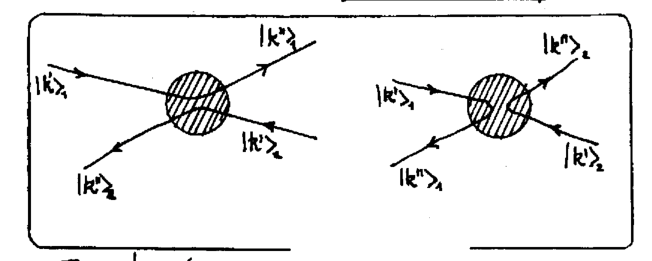
\includegraphics[width=0.9\textwidth]{images/teo2_29.pdf}
	\end{center}
	\caption{}
\end{figure} 
Entonces un estado general será
\[
	=
\]
Esta es la ``degeneración de intercambio''.

\subsection{Permutación}

Definimos este operador como 
\[
	P_{12} =
\]
\[
	P
\]
Su función es la de intercambiar etiquetas, no el orden de las partículas.
Sean operadores $\hat{A}_1,\hat{A}_2$ que actúan sobre las partículas 1,2; es decir 
\[
	a
\]
\[
	b
\]
\[
	c
\]

Luego $\hat{A}$ es simétrico si $[\hat{P}_{12},\hat{A}_{12}]=0$. Sea $[\hat{P}_{12},\hat{H}]=0$ entonces es 
$P_{12}$ constante de movimiento y 
\[
	P
\]
Sea 
\[
	H = 
\]
y defino dos estados
\[
	a
\]
con 
\[
	as
\]
Puedo introducir operadores de simetrización y antisimetrización 
\[
	S A
\]
\[
	S
\]
\[
	A
\]
En general se complica bastante con más de dos partículas 
\[
	P_{ij}
\]
pués tenemos 
\[
	[P_{ij},P_{k\ell}] \neq 0 \text{en general}
\]
Las permutaciones para tres partículas pueden descomponerse 
\[
	P
\]

Con tres partículas hay $3!$ estados
\[
	estados 
\]
En estados simétricos serán 
\[
	\Braket{} =
\]
donde el $\Braket{}_A$ tiene el signo $(-)$ en las permutaciones anticíclicas y el $(+)$ en las cíclicas.
Existe un determinante de Slater como método mnemotécnico de obtener los estados $\Braket{}_A$.
\[
	\Ket{ \Psi }_A = \frac{1}{3!}
\]
La obtención de estos estados corresponde a aplicar 
\[
	A_{123} =
\]
Si dos $k^{(i)}$ coinciden ya no hay estado antisimétrico posible.

\section{Postulado de simetrización}

Permitirá romper la degeneración de intercambio. 
Postulamos que toda partícula es de uno de dos tipos de acuerdo a su simetría 

\begin{center}
\begin{tabular}{llll}
N & simetrica & BE & entero\\
N & antisimetrica & FD & semientero
\end{tabular}
\end{center}

En la naturaleza no ocurren simetrías mixtas.

\subsection{Principio de exclusión de Pauli}

Para fermiones supongamos sistema de dos partículas idénticas 
\[
	\Psi
\]

No es posible tener dos fermiones con iguales números cuánticos. Por el contrario los bosones sí pueden tener 
iguales números cuánticos.

\subsection{Sistema de dos electrones de spin $1/2$}

Sistema de dos electrones de spin $1/2$. Son fermiones. Sea que $[H,S]=0$  con $S = S_1 + S_2$. Se tendrá 
\[
	Psi
\]
Como $\Ket{\Psi}^{sist}$ es simétrica tendremos 
\[
	P
\]
\[
	P
\]

Para dos electrones con spin $1/2$ se tiene 
\[
	a
\]
\[
	b
\]
\[
	c
\]
Entonces 
\[
	a
\]
Vistos desde el CM de los electrones
\[
	P
\]
\[
	Q
\]
Necesitaré $\ell$ par con $s=0$ entonces $\ell+s=j$ par. En cambio, si $\ell$ impar con $s=1$ entonces 
$\ell+s=j$ par. Dos electrones sólo se acoplan a momento total $j$ par.

Sean los siguientes estados 
\[
	Psi
\]
\[
	Psi2
\]
y la probabilidad será
\[
	Prob
\]
\[
	a
\]
\[
	b
\]
\[
	Prob
\]

Vemos que aparece una interferencia que será importante solamente si hay solapamiento. En el caso de no 
solaparse o con partículas clásicas solo el primer término es de importancia.

\section{El átomo de helio}


\begin{figure}[htb]
	\begin{center}
	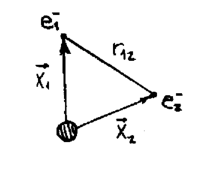
\includegraphics[width=0.4\textwidth]{images/teo2_30.pdf}
	\end{center}
	\caption{}
\end{figure} 
\[
	H = 
\]
en este último caso $H$ está desacoplado 
\[
	\Psi = 
\]
\[
	[]
\]
S es constante de movimiento y para la $\Ket{\psi_{spin}}$ se tiene 
\[
	a
\]
\[
	b
\]
\[
	c
\]
\[
	d
\]

Podemos pensar en teoria de perturbaciones ahora y calcular 
\[
	E_{He} = 
\]
donde 
\[
	\Delta E = 
\]
lo considero una perturbación.
\[
	a
\]
\[
	d
\]
\[
	\Delta E = I \pm J
\]

\begin{figure}[htb]
	\begin{center}
	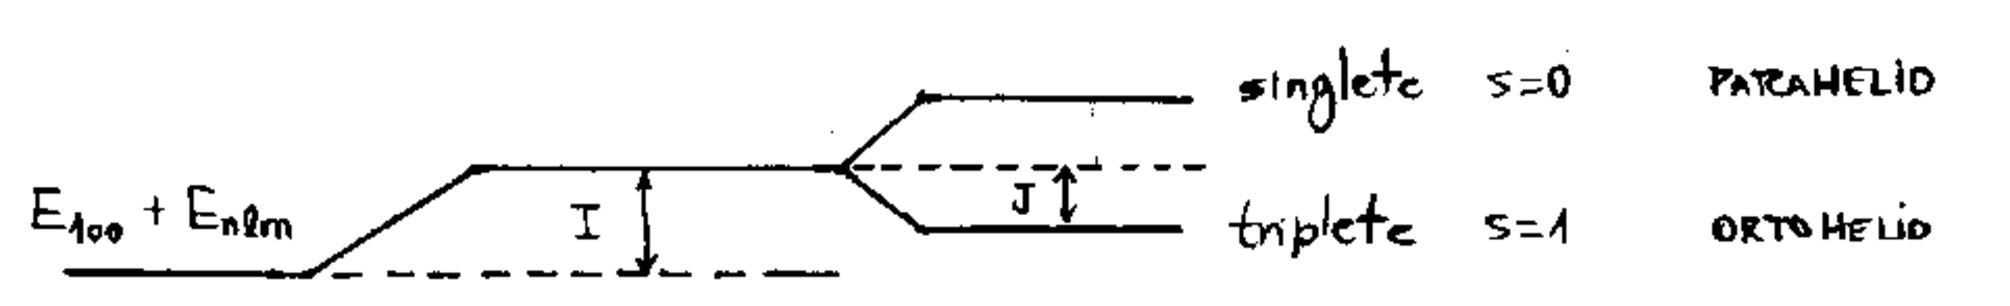
\includegraphics[width=1.0\textwidth]{images/teo2_15.pdf}
	\end{center}
	\caption{}
\end{figure} 

Esta separación de los niveles en $\pm J$ se debe al carácter de fermión de las partículas.



% \bibliographystyle{CBFT-apa-good}	% (uses file "apa-good.bst")
% \bibliography{CBFT.Referencias} % La base de datos bibliográfica

\end{document}

	
		\documentclass[10pt,oneside]{CBFT_book}
	% Algunos paquetes
	\usepackage{amssymb}
	\usepackage{amsmath}
	\usepackage{graphicx}
	\usepackage{libertine}
	\usepackage[bold-style=TeX]{unicode-math}
	\usepackage{lipsum}

	\usepackage{natbib}
	\setcitestyle{square}

	\usepackage{polyglossia}
	\setdefaultlanguage{spanish}
	



	\usepackage{CBFT.estilo} % Cargo la hoja de estilo

	% Tipografías
	% \setromanfont[Mapping=tex-text]{Linux Libertine O}
	% \setsansfont[Mapping=tex-text]{DejaVu Sans}
	% \setmonofont[Mapping=tex-text]{DejaVu Sans Mono}

	%===================================================================
	%	DOCUMENTO PROPIAMENTE DICHO
	%===================================================================

\begin{document}




% =================================================================================================
\chapter{Picture de interacción y perturbación dependiente del tiempo}
% =================================================================================================

Puédense escribir perturbaciones dependientes del tiempo 
\[
	H = H_0 + V(t)
\]
con $\Ket{n}$ no dependiente del tiempo. Se estudiarán transiciones entre autoestados del $H_0$ (que son 
estacionarios). Un autoestado permanece en el tiemo como tal pero con fase oscilante
\[
	\Ket{\alpha,t_0,t}_s = \euler^{-iH/\hbar(t-t_0)}\Ket{\alpha,t_0}_s
\]
\[
	= \euler^{-iH/\hbar(t-t_0)} \euler^{-iV(t)/\hbar(t-t_0)} \Ket{\alpha,t_0}
\]
\[
	= \sum_n \euler^{-iH_0/\hbar \: t} \euler^{-iV(t)/\hbar \: t} \ket{n}\Braket{n|\alpha,t_0}
\]
\[
	= \sum_n \euler^{-iE_n^0/\hbar \: t }\ket{n}\euler^{-iV(t)/\hbar \: t } \Braket{n|\alpha,t_0}	
\]
\[
	\euler^{iH_0/\hbar t}\Ket{\alpha,t_0,t}_s =
	\sum_n  \underbrace{\euler^{-iV(t)/\hbar \: t} \Braket{n|\alpha,t_0}}_{C_n(t)} \ket{n} = \Ket{\alpha,t_0,t}_I	
\]
es decir 
\[
	 \Ket{\alpha,t_0,t}_I = \euler^{iH_0/\hbar t}\Ket{\alpha,t_0,t}_s
\]
Aquí se puede pensar que 
\begin{itemize}
 \item $C_n(t)$ evoluciona por $V(t)$
 \item $\euler^{-iE_n^0 t/\hbar}$ evoluciona por $H_0$
\end{itemize}

Esto introduce la {\it picture} de interacción de Dirac; en la cual los estados evolucionan con $V(t)$.

\begin{center}
\begin{tabular}{|c|ccc|}
\hline 
& Dirac & Schrödinger & Heinsenberg \\
\hline 
% & &  & \\
estados & evolucionan & evolucionan & fijos \\
$\Ket{\alpha}$ & con $V(t)$ & con $H$ &  \\
\hline
operadores & evolucionan & fijos & evolucionan \\
 & con $H_0$ &  & con $H$ \\
\hline
base & fijos & fijos & evolucionan \\
$\Ket{a'}$ &  &  &  \\
\hline 
% & & & \\
\end{tabular}
\end{center}

\[
	i\hbar \dpar{}{t}\Ket{\alpha,t_0,t}_s = H \Ket{\alpha,t_0,t}_s
\]
\[
	i\hbar \dpar{}{t}\left( \euler^{-iH_0t/\hbar}\Ket{\alpha,t_0,t}_I \right) = 
	H \euler^{-iH_0t/\hbar} \Ket{\alpha,t_0,t}_I
\]
\[
	i\hbar \euler^{-iH_0t/\hbar}\dpar{}{t} \Ket{\alpha,t_0,t}_I = 
	V(t) \euler^{-iH_0t/\hbar} \Ket{\alpha,t_0,t}_I
\]
\[
	i\hbar \dpar{}{t} \Ket{\alpha,t_0,t}_I = V(t) \Ket{\alpha,t_0,t}_I,
\]
que es la ecuación de evolución de los kets.
Pediremos asimismo que 
\[
	_s\Braket{\; A_s \;}_s = _I\Braket{\; A_I \;}_I
\]
\[
	_I\Braket{\alpha,t_0,t|A_I|\alpha,t_0,t}_I =
	_s\Braket{\alpha,t_0,t|\euler^{-iH_0t/\hbar}A_I\euler^{iH_0t/\hbar}|\alpha,t_0,t}_s=
	_s\Braket{\alpha,t_0,t|A_s|\alpha,t_0,t}_s =
\]
Y los operadores evolucionan según 
\[
	A_I = \euler^{iH_0t/\hbar}A_s\euler^{-iH_0t/\hbar}
\]
\[
	\dtot{A_I}{t} = \frac{1}{i\hbar}[A_I, H_0]
\]
que es igual que la ecuación de Heisenberg pero con $\hat{H}_0$ en lugar de $H$.
Los kets base permanecen fijos, porque así lo hacen en Schrödinger, en realidad oscila su fase; entonces 
\[
	\Ket{n,t_0,t}_s = \euler^{-iHt/\hbar} \ket{n,t_0}_s
\]
\[
	\Ket{n,t_0,t}_I = \euler^{iH_0t/\hbar} \euler^{-iHt/\hbar} \ket{n,t_0}_s =
	\euler^{-iVt/\hbar} \ket{n,t_0}_s = \euler^{iH_0t/\hbar} \ket{n,t_0}_s
\]
\[
	\Ket{n,t_0,t}_I = \euler^{iE_0t/\hbar} \ket{n,t_0,t}_s
\]

\subsection{Evolución de los coeficientes}

\[
	as
\]
\[
	C_n(t) =
\]
\[
	d
\]
y le pego un $\Bra{n}$ a la ecuación de evolución de kets,
\[
	i\hbar
\]
\[
	s
\]
\[
	i\hbar
\]
donde $V_{nm}(t) \equiv \Braket{n|V(t)|m}$ y $\omega_{nm} \equiv (E_n-E_m)/\hbar$.
Esta es la ecuación que cumplen los coeficientes, donde $|C_n(t)|^2$ es la probabilidad de hallar al sistema 
en el autoestado $\Ket{n}$.
Es decir
\[
	\begin{matrix}
	 =
	\end{matrix}
\]
que puede ser de difícil solución.

\subsection{Método perturbativo (dependiente del tiempo)}

Pensaremos en una serie perturbativa 
\[
	C_n(t) =
\]

El evolucionador temporal en la picture de interacción cumple 
\[
	\Ket{} =
\]
que viene de  
\[
	i\hbar
\]
la cual resolviendo nos hace llegar a 
\[
	U
\]
y esto lleva a la serie de Dyson:
\[
	U
\]

\subsection{Transiciones entre autoestados del hamiltoniano $H_0$}
\[
	\Ket{} =
\]
\[
	a
\]
La amplitud de transición será 
\[
	C
\]
con $\Ket{i},\Ket{n}$ autoestados de $H_0$.
Sea $\tilde{C}_n(t)=\Braket{n|U_s(t)|i}$ y busquemos una expresión 
\[
	a
\]
\[
	b
\]
y notemos que $\hat{U}$ no obedece la ley de transformación de operadores.

\[
	a
\]
\[
	b \Rightarrow |C_n(t)|^2 = |\tilde{C}_n(t)|^2
\]

Para transiciones entre autoestados de $H_0$ los coeficientes dan la misma probabilidad (evaluados con el 
evolucionador de Dirac que con el de Schrödinger).
Vamos a las transiciones a los tres 
\begin{itemize}
 \item orden 0
 \item orden 1
 \item orden 2
\end{itemize}

\subsection{Ejemplo: potencial constante encendido abruptamente}

Notemos que $V\neq V(t)$. Dependerá de cualquier otra cosa.
\[
	a
\]
\[
	b
\]
\begin{figure}[htb]
	\begin{center}
	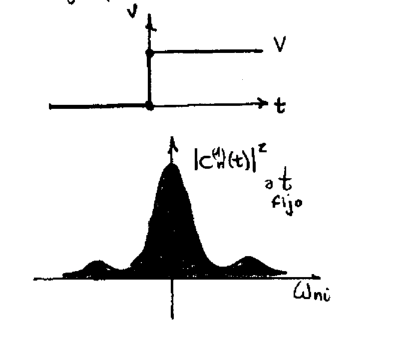
\includegraphics[width=0.6\textwidth]{images/teo2_22.pdf}
	\end{center}
	\caption{}
\end{figure} 
Es máxima la probabilidad cuando $\Delta E\to 0$. En ese caso las transiciones son a estados de la misma 
energía. A tiempo largo la probabilidad es no nula para aquellos estados 
\[
	t \sim \frac{2\pi}{|\omega_{ni}|}
\]
Hay probababilidad de transición $\Ket{i} \to \Ket{n}$ apreciable con $\Delta E \sim 0$.

\section{Scattering: orden 1}

Este último ejemplo puede aplicarse a colisiones elásticas. Prendemos y apagamos un potencial que es el 
masacote al cual impactamos. De entrada ha partículas libres y de salida (lejos de $V$) partículas libres.
Entonces $ E_n - E_c \sim 0$ y consideraremos lo que sucede a tiempos largos. Interesará la probabilidad 
total de transicionear a estados de energía similares a $E_i$. Por ello se considera 
\[
	\sum 
\]
donde el integrando es el número de estados dentro de un intervalo de energías $(E,E+dE)$.
\begin{figure}[htb]
	\begin{center}
	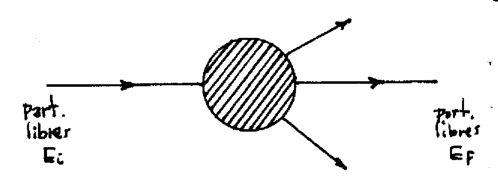
\includegraphics[width=0.6\textwidth]{images/teo2_23.pdf}
	\end{center}
	\caption{}
\end{figure} 
En tiempos muy largos la expresión [1] tiende a una delta de Dirac y se integra fácil,
\[
	\lim 
\]

La probabilidad de transición es proporcional a $t$. Se suele definir una tasa de transición (probabilidad de 
transición por unidad de tiempo)
\[
	\dtot{}{t}\left( \sum_{n(E_n\sim E_i)} |C_n^1|^2 \right) =
\]
que es la regla de oro de Fermi.

\section{El método variacional}

Se puede usar para aproximar la energía del estado fundamental (el estado de energía mínima)
\[
	=
\]
\[
	=
\]
y usamos 
\[
	\frac{|}{|} \geq E_0
\]

\subsection{Scattering a orden dos y OFPT}

Continuando con el orden dos de scattering por un $V\neq V(t)$ se tiene:
\[
	\omega
\]

Para obtener los siguientes términos dentro del $\bar{||^2}$ podemos emplear un ardid gráfico conocido como 
{\it Old Fashioned Perturbation Theory}

\begin{figure}[htb]
	\begin{center}
	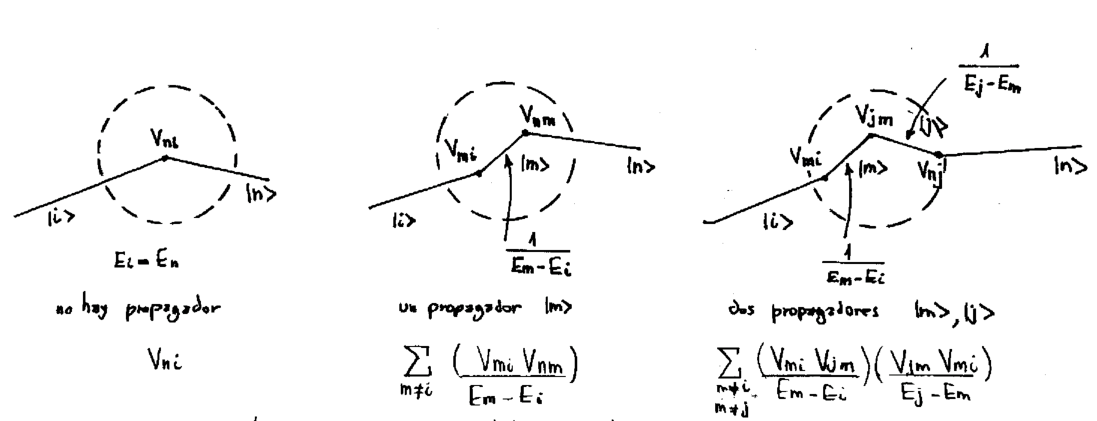
\includegraphics[width=1.0\textwidth]{images/teo2_24.pdf}
	\end{center}
	\caption{}
\end{figure} 


Fíjese que en los estados intermedios estados virtuales $\Ket{m},\Ket{j}$ no se conserva la energía. Son 
propagadores.


\subsection{Perturbación armónica}

Sea un potencial armónico y hermítico 
\[
	V(t) =
\]
quiero ver probabilidad de transición a orden uno,
\[
	C_n(t)^1 = 
\]
\[
	a
\]
\[
	b
\]
\[
	c
\]

Luego será nulo sólo si 
\[
	\omega
\]
\[
	\omega
\]

\begin{figure}[htb]
	\begin{center}
	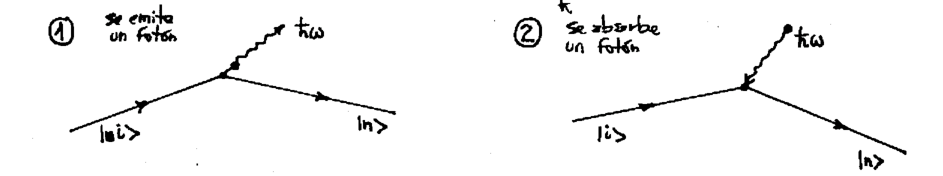
\includegraphics[width=1.0\textwidth]{images/teo2_25.pdf}
	\end{center}
	\caption{}
\end{figure} 

Luego,
\[
	\lim 
\]
representa la probababilidad de emitir o absorber fotones en una interacción. Se puede asociar que $V$ crea 
fotones y $V^\dagger$ destruye fotones. Para un átomo se tiene 
\begin{figure}[htb]
	\begin{center}
	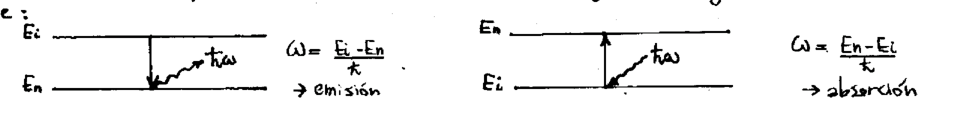
\includegraphics[width=1.0\textwidth]{images/teo2_26.pdf}
	\end{center}
	\caption{}
\end{figure} 




\section{Despoblamiento de estados iniciales}

Queremos ver con cual $v$ se despoblan los $\Ket{i}$. Para elllo me construyo un potencial {\it suave}
\[
	\lim 
\]
donde $\eta$ es un parámetro regularizador.
\begin{figure}[htb]
	\begin{center}
	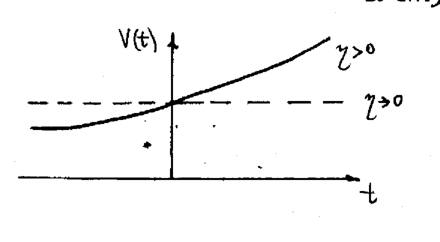
\includegraphics[width=0.6\textwidth]{images/teo2_27.pdf}
	\end{center}
	\caption{}
\end{figure} 
\[
	a
\]
\[
	b
\]
\[
 	c
\]
y tomando el límite $\eta \to 0$ 
\[
	d
\]
y llegamos a la regla de oro de Fermi,
\[
	d
\]

\subsection{Scattering sección eficaz}

$\Ket{k},\Ket{k}'$ son autoestados de momento (partículas libres),
\[
	|\vb{k}| = |\vb{k}'| 
\]
se conserva la energía. Consideraremos la aproximación más baja (aproximación de Born).
\begin{figure}[htb]
	\begin{center}
	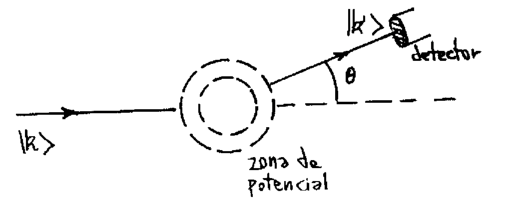
\includegraphics[width=0.6\textwidth]{images/teo2_28.pdf}
	\end{center}
	\caption{}
\end{figure} 

\[
	\omega 
\]
queremos calcular la densidad de estados de energía entre $(E,E+dE)$. Pensamos en una partícula libre en una 
caja $1D$ de longitud $L$.
\[
	N
\]
pidiendo normalización unitaria $\Braket{k|k}=1$ se tiene 
\[
	d
\]
con $L\to\pm\infty$ son $n_x,k_x$ continuas.
\[
	d
\]
\[
	d
\]
donde $n^2\:dn\:d\Omega$ es la densidad de estados de energía $(E,E+dE)$ en $d\Omega$
\[
	n^2 \: dn \: d\Omega = \rho(E') dE'
\]

Con esto sale la integral obteniéndose
\[
	\omega_{\vb{k}-\vb{k}'} = 
	\frac{L^3}{(2\pi)^2} \frac{m}{\hbar^3} \left|\Braket{\vb{k}'|V|\vb{k}}\right|^2 k'd\Omega
\]

Esta es la probabilidad de transición entre los impulsos $\vb{k}$, $\vb{k}'$. Es el número de partículas en 
la unidad de tiempo por unidad de área 
\[
	\text{seccion eficaz} \equiv \dtot{\sigma}{\Omega}d\Omega =
	\frac{\text{\# de part en $d\Omega$ en la unidad de t}}
	{\text{\# de part incidentes en la unidad de t por unidad de área}}
\]

Un elemento de matriz $\Braket{k'|V|k}$ será 
\[
	\Braket{\vb{k}'|V|\vb{k}} = \int dx'\Braket{\vb{k}'|\vb{x}'} \Braket{\vb{x}'|V|\vb{k}} =
	\int d\vb{x}' \frac{1}{L^3} \euler^{i (\vb{k}-\vb{k}')\cdot \vb{x}} \; V(\vb{x}'),
\]
\begin{figure}[htb]
	\begin{center}
	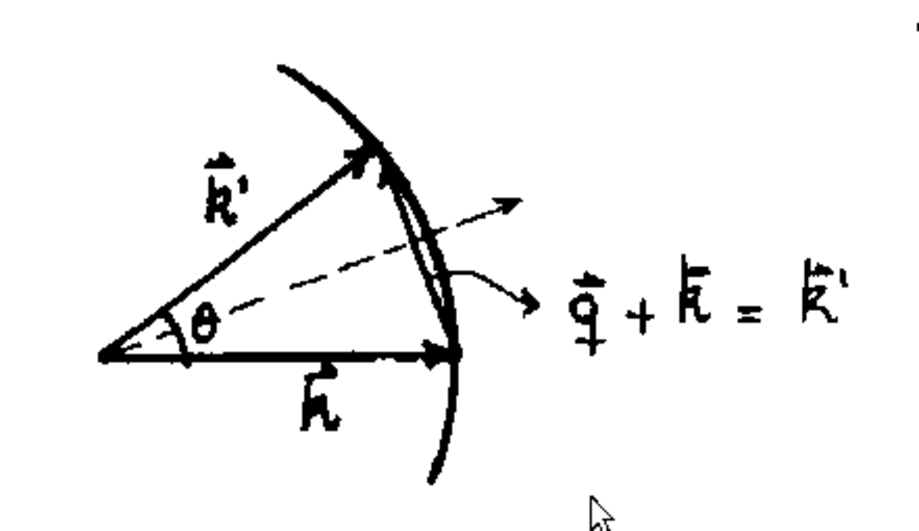
\includegraphics[width=0.5\textwidth]{images/teo2_31.pdf}
	\end{center}
	\caption{}
\end{figure} 
la transformada de Fourier del potencial es, amén de constantes, la amplitud a primer orden 
\[
	|\vb{k} - \vb{k}'| = 2k\sin(\theta/2) \qquad \text{con} \; k=k' 
\]
Entonces para cualquier potencial esféricamente simétrico se puede hacer la integral 
\[
	\dtot{\sigma}{\Omega} =
	\left|\left( \frac{2m}{4\pi\hbar}\right)^2 \int d^3x'\;V(x)\euler^{i(\vb{x}-\vb{x}')\cdot\vb{x}'}\right|^2
\]
y expresamos todo en función de $q=q(\theta)$
\[
	\dtot{\sigma}{\Omega} =
	\left| -\frac{2m}{\hbar^2} \frac{1}{q} \int_0^\infty rV(r)\sin(q) dr \right|^2
\]

Utilizando un potencial de Yukawa primero y tomando el límite para llegar al de Coulomb tenemos la sección 
eficaz de Rutherford 
\[
	\dtot{\sigma}{\Omega} = \frac{2m^2e^4}{\hbar^4}\frac{1}{16k^4\sin^4(\theta/2)}
\]

hay que tomar el potencial de Yukawa y luego el límite porque el de Coulomb diverge de entrada



% \bibliographystyle{CBFT-apa-good}	% (uses file "apa-good.bst")
% \bibliography{CBFT.Referencias} % La base de datos bibliográfica

\end{document}

	
		\documentclass[10pt,oneside]{CBFT_book}
	% Algunos paquetes
	\usepackage{amssymb}
	\usepackage{amsmath}
	\usepackage{graphicx}
	\usepackage{libertine}
	\usepackage[bold-style=TeX]{unicode-math}
	\usepackage{lipsum}

	\usepackage{natbib}
	\setcitestyle{square}

	\usepackage{polyglossia}
	\setdefaultlanguage{spanish}
	



	\usepackage{CBFT.estilo} % Cargo la hoja de estilo

	% Tipografías
	% \setromanfont[Mapping=tex-text]{Linux Libertine O}
	% \setsansfont[Mapping=tex-text]{DejaVu Sans}
	% \setmonofont[Mapping=tex-text]{DejaVu Sans Mono}

	%===================================================================
	%	DOCUMENTO PROPIAMENTE DICHO
	%===================================================================

\begin{document}

% =================================================================================================
\chapter{Introducción a la mecánica cuántica relativista}
% =================================================================================================

Consideremos una partícula libre por el momento 
\[
	H = \frac{p^2}{2m} \quad E =  i\hbar \dpar{}{t} \quad \vb{p} = - i\hbar \Nabla
\]
en relatividad la primera expresión no sirve pero la segunda y la tercera sí.
\[
	P_\mu = i \hbar \partial_\mu = i \hbar \dpar{}{x^\mu}
\]
\[
	p^\mu = (E/c, \vb{p}) \qquad p_\mu = (E/c, -\vb{p}) \qquad x^\mu = (ct, \vb{x})
\]
\[
	\dpar{}{x^\mu} = \left( \frac{1}{c}\dpar{}{t} , \Nabla \right) \equiv \partial_\mu
	\qquad \dpar{}{x_\mu} = \left( \frac{1}{c}\dpar{}{t} , -\Nabla \right) \equiv \partial^\mu
\]
y Schrödinger para la partícula libre es
\be \label{schro_freepart}
	i \hbar \dpar{\psi}{t} = - \frac{\hbar^2}{2m} \nabla^2 \psi
\ee
y entonces podemos hacer la cuenta 
\[
	\psi^* \times \eqref{schro_freepart} \rightarrow  
	i \hbar \psi^*\dpar{\psi}{t} = - \frac{\hbar^2}{2m} \psi^* \nabla^2 \psi
\]
y conjugando la ecuación,
\[
	\psi \times \eqref{schro_freepart}^* \rightarrow  
	-i \hbar \psi\dpar{\psi^*}{t} = - \frac{\hbar^2}{2m} \psi \nabla^2 \psi^*
\]
y restando ambas expresiones se obtiene 
\[
	i \hbar \left( \psi^*\dpar{\psi}{t} + \psi\dpar{\psi^*}{t} \right) =
	\frac{\hbar^2}{2m} \left( \psi \nabla^2 \psi^* -\psi^* \nabla^2 \psi \right)
\]
\[
	i \hbar  \dpar{ (\psi^* \psi) }{t} + \frac{\hbar^2}{2m} 
	\Nabla \cdot \left( \psi^* \Nabla \psi - \psi \Nabla \psi^* \right) = 0
\]
la cual se puede reescribir como
\[
	\dpar{ (\psi^* \psi) }{t} +  
	\Nabla \cdot \left( \frac{\hbar}{2mi} [\psi^* \Nabla \psi - \psi \Nabla \psi^*] \right) = 0
\]
que es una analogía de la conservación de la carga en electrodinámica. Recordemos que la conservación de la carga era
$ \partial_t \rho + \nabla \cdot \vb{J} = 0$.
Tenemos entonces una especie de conservación de la probabilidad. Note que $\psi^* \psi = |\psi|^2 \geq 0$
\[
	E^2 = c^2 p^2 + m^2 c^4
\]
\[
	E = \sqrt{ c^2 p^2 + m^2 c^4 } = H \qquad \text{con} \; H\psi = E\psi
\]

Pero esto se pone muy complicado debido a la raíz

\subsection{La ecuación de Klein-Gordon}

Conserva el cuadrado para no complicar demasiado los reemplazos. Entonces 
\[
	H^2 = E^2 = c^2p^2 + m^2c^4
\]
\be \label{ec_kg}
	-\hbar \dpar[2]{\psi}{t} = - \hbar^2c^2 \Nabla^2\psi + m^2 c^4 \psi
\ee
\[
	p^\mu p_\mu = m^2c^2 \qquad -\partial_\mu\partial^\mu \psi = \frac{m^2c^2}{\hbar^2}\psi
\]
siendo el operador $\Box^2 \equiv \partial_\mu\partial^\mu$ el dalembertiano.
\[
	\left( \Box^2 + \frac{m^2c^2}{\hbar^2} \right) \psi = 0
\]
y procediendo de modo ídem al caso anterior,
\[
	\psi^* \cdot \eqref{ec_kg} = - \hbar^2 \psi^* \partial_t^2 \psi =
	- \hbar^2 c^2 \psi^* \nabla^2 \psi + m^2 c^4 \psi^*\psi
\]
\[
	\psi \cdot \eqref{ec_kg}^* = - \hbar^2 \psi \partial_t^2 \psi^* =
	- \hbar^2 c^2 \psi \nabla^2 \psi^* + m^2 c^4 \psi\psi^*
\]
y restando ambas ecuaciones tenemos
\[
	\hbar^2 \dpar{}{t}\left(  \psi^* \partial_t \psi -  \psi \partial_t \psi^* \right) =
	\hbar^2 c^2 \Nabla\cdot( \psi^* \Nabla \psi - \psi \Nabla \psi^* )
\]
\[
	\dpar{}{t}\left( \frac{i}{c^2}[ \psi^* \partial_t \psi -  \psi \partial_t \psi^* ]\right) +
	i\Nabla\cdot( \psi \Nabla \psi^* - \psi^* \Nabla \psi ) = 0
\]

El problema es que no puede asegurarse que esta $\rho \equiv i/c^2[ \psi^* \partial_t \psi -  \psi \partial_t 
\psi^* ]$ sea definida positiva, lo cual sería necesario para seguir una coherencia.
\[
	\psi = N \euler^{ i/\hbar(\pe{p}{x} - Et)}
\]
\[
	\partial_t \psi = -N \frac{iE}{\hbar} \euler^{ i/\hbar(\pe{p}{x} - Et)}
\]
\[
	\rho = \frac{i}{c^2}\left( N^*\euler^{ -i/\hbar(\pe{p}{x} - Et)}(-N)
	\frac{iE}{\hbar} \euler^{ i/\hbar(\pe{p}{x} - Et)} - 
	N \euler^{ i/\hbar(\pe{p}{x} - Et)}N^*\frac{E}{\hbar} \euler^{ i/\hbar(\pe{p}{x} - Et)}\euler^{i\pi/2}
	\right)
\]
\[
	\rho = -\frac{i}{c^2}\left( 2|N|^2 \frac{iE}{\hbar} \right) < 0 \quad \text{si} \quad E > 0
\]
para una onda plana.
Necesito considerar $E<0$ pues $E=\pm\sqrt{c^2p^2+m^2c^4}$ y la base debe ser completa.

La densidad $\rho$ es positiva si tuviese $E<0$ pero esto causa el problema de tener materia inestable, pues nunca se 
alcanza el fundamental. Acá muere en este atolladero la ecuación de Klein-Gordon.

\subsection{La ecuación de Dirac}

Dirac parte de pedir una ecuación lineal en el impulso \vb{p}
\[
	H = c \vb{\alpha} \cdot \vb{p} + \beta m c^2
\]
usando $H\psi = E\psi$ y $H^2 = E^2 = c^2p^2 + ,m^2 c^4$ y con $\beta,\vb{\alpha},\vb{p}$ operadores.
\[
	H^2 = (c \vb{\alpha} \cdot \vb{p} + \beta m c^2)(c \vb{\alpha} \cdot \vb{p} + \beta m c^2)
\]
\[
	H^2 = c^2 \alpha_i p_i \alpha_\ell p_\ell + c^3 \alpha_i p_i \beta m +
	\beta m c^3 \alpha_i p_i + \beta^2 m^2 c^4
\]
\[
	H^2 = c^2 \alpha_i \alpha_\ell p_i  p_\ell + c^3 m p_i \underbrace{( \alpha_i \beta + \beta \alpha_i )}_{=0}
	+ \beta^2 m^2 c^4
\]
\[
	H^2 = 
	c^2 \underbrace{\left( \frac{\alpha_i \alpha_\ell + \alpha_\ell\alpha_i}{2} \right)}_{\delta_{i\ell}}
	p_i p_\ell + m^2 c^4 \underbrace{\beta^2 }_{ = 1 }
\]
\[
	\alpha_i \alpha_\ell + \alpha_\ell\alpha_i = 2 \delta_{i\ell} \qquad 
	\alpha_i \beta + \beta \alpha_i= 0 \qquad
	\beta^2 = 1
\]
Como se ve, estos no pueden ser simples escalares. Dirac pide 
\begin{itemize}
 \item $\vb{\alpha},\beta$ hermíticos
 \item $\beta^2=1 \; \alpha^2=1$ autovalores $\pm 1$
 \item traza nula
 \[
	\alpha_i \beta = -\beta \alpha_i  \quad \rightarrow  \quad 
	\beta \alpha_i \beta = -\beta^2 \alpha_i = -\alpha_i
 \]
 \[
	Tr(\alpha_i) = -Tr(\beta \alpha_i \beta) = -Tr(\beta\beta\alpha_i)
 \]
 \item dimensión par 
 \[
	\vb{\alpha} = \begin{pmatrix} 0 & \vec{\sigma} \\ \vec{\sigma} & 0 \\ \end{pmatrix} \qquad 
	\beta = \begin{pmatrix} \mathbb{1} & 0 \\ 0 & -\mathbb{1} \\ \end{pmatrix}
 \]
 donde cada elemento de la matriz es de $2\times2$.
\end{itemize}

Entonces
\[
	H \vec{\psi} = i \hbar \dpar{\vec{\psi}}{t}, \qquad H \in 4\times 4, \vec{\psi} \in 4\times 1, \qquad
	\vec{\psi} = \begin{pmatrix} \psi_1 \\ \psi_2 \\ \psi_3 \\ \psi_4 \end{pmatrix}
\]
\be \label{ec_dirac}
	i \hbar \dpar{\psi}{t} = -i \hbar c \sum_k \alpha_k \dpar{\psi}{x_k} + m c^2 \beta \psi
\ee
\[
	-i \hbar \dpar{\psi^\dagger}{t} = i \hbar c \sum_k \dpar{\psi^\dagger}{x_k}\alpha_k + m c^2\psi\alpha_k\beta
\]
\[
	\psi^\dagger\cdot\eqref{ec_dirac} - \eqref{ec_dirac}^\dagger\cdot \psi \rightarrow 
	i\hbar \dpar{}{t}(\psi^\dagger psi) = -i\hbar c \sum_k \dpar{}{x_k}(\psi^\dagger \alpha_k \psi)
\]
\[
	\dpar{}{t}(\psi^\dagger psi) + c \sum_k \dpar{}{x_k}(\psi^\dagger \alpha_k \psi) = 0
\]
Y si $\rho \equiv \psi^\dagger\psi$ ahora tenemos una densidad de proababilidad como requiere la naturaleza.

\subsection{Ejemplo: partícula libre quieta}

Sea una partícula libre en reposo,
\[
	\vb{p} = 0 \qquad H=\beta m c^2
\]
\[
	i \hbar \dpar{\psi}{t} = \beta m c^2 \psi
\]
\[
	i \hbar \dpar{}{t} \begin{pmatrix} \psi_1 \\ \psi_2 \\ \psi_3 \\ \psi_4  \end{pmatrix} =
	\begin{pmatrix} mc^2 & 0 & 0 & 0 \\ 0 & mc^2 & 0 & 0 \\ 0 & 0 & -mc^2 & 0 \\ 0 & 0 & 0 & -mc^2 \end{pmatrix}
	\begin{pmatrix} \psi_1 \\ \psi_2 \\ \psi_3 \\ \psi_4  \end{pmatrix}
\]
Tenemos cuatro ecuaciones, dos con energía positiva y dos con energía negativa
\[
	i \hbar \dpar{\psi_i}{t} = mc^2 \psi_i \qquad i \hbar \dpar{\psi_i}{t} = -mc^2 \psi_i
\]
\[
	\psi_1 = \euler^{-imc^2t/\hbar}\begin{pmatrix} 1 \\ 0 \\ 0 \\ 0  \end{pmatrix} \qquad 
	\psi_3 = \euler^{imc^2t/\hbar}\begin{pmatrix} 0 \\ 0 \\ 1 \\ 0  \end{pmatrix}
\]
Como aún tenemos degeneración de orden dos, necesitaremos un operadore que conmute con el $H$
\[
	\vec{\Sigma} = \begin{pmatrix} \vec{\sigma} & 0 \\ 0 & \vec{\sigma} \\ \end{pmatrix} \qquad 
	[H,\vec{\Sigma}] = 0
\]
\[
	\Sigma_3 =  \begin{pmatrix} \sigma_3 & 0 \\ 0 & \sigma_3 \\ \end{pmatrix} = 
	\begin{pmatrix} 1 & 0 & 0 & 0 \\ 0 & -1 & 0 & 0 \\ 0 & 0 & 1 & 0 \\ 0 & 0 & 0 & -1 \end{pmatrix}
\]
\begin{align*}
	\psi_1, E=mc^2, \Sigma_3=1 \qquad  &\psi_2, E=mc^2, \Sigma_3=-1 \\
	\psi_3, -E=mc^2, \Sigma_3=1 \qquad  &\psi_4, -E=mc^2, \Sigma_3=-1
\end{align*}
Podemos identificar 
\[
	\vec{S} = \frac{\hbar}{2} \vec{\Sigma}
\]
\[
	\text{si} \; p \neq 0  \Rightarrow [H, \vb{\Sigma}] = 2ic \vb{\alpha} \times \vb{p}
\]

\subsection{Energías negativas}

Como $E = \pm  \sqrt{ c^2 p^2 + m^2 c^4 } $ hay $E<0$ y además un {\it gap} de ancho $2mc^2$ entre ellas.
Las $E<0$ harían que la materia jamás alcance un estado fundamental y por ende jamás se estabilice.
Dirac piensa que los estados de $E<0$ están todos llenos. No decaen más electrones allí dentro. Es el mar de 
Dirac. Iluminando ese vacío se lo puede excitar.

\begin{figure}[htb]
	\begin{center}
	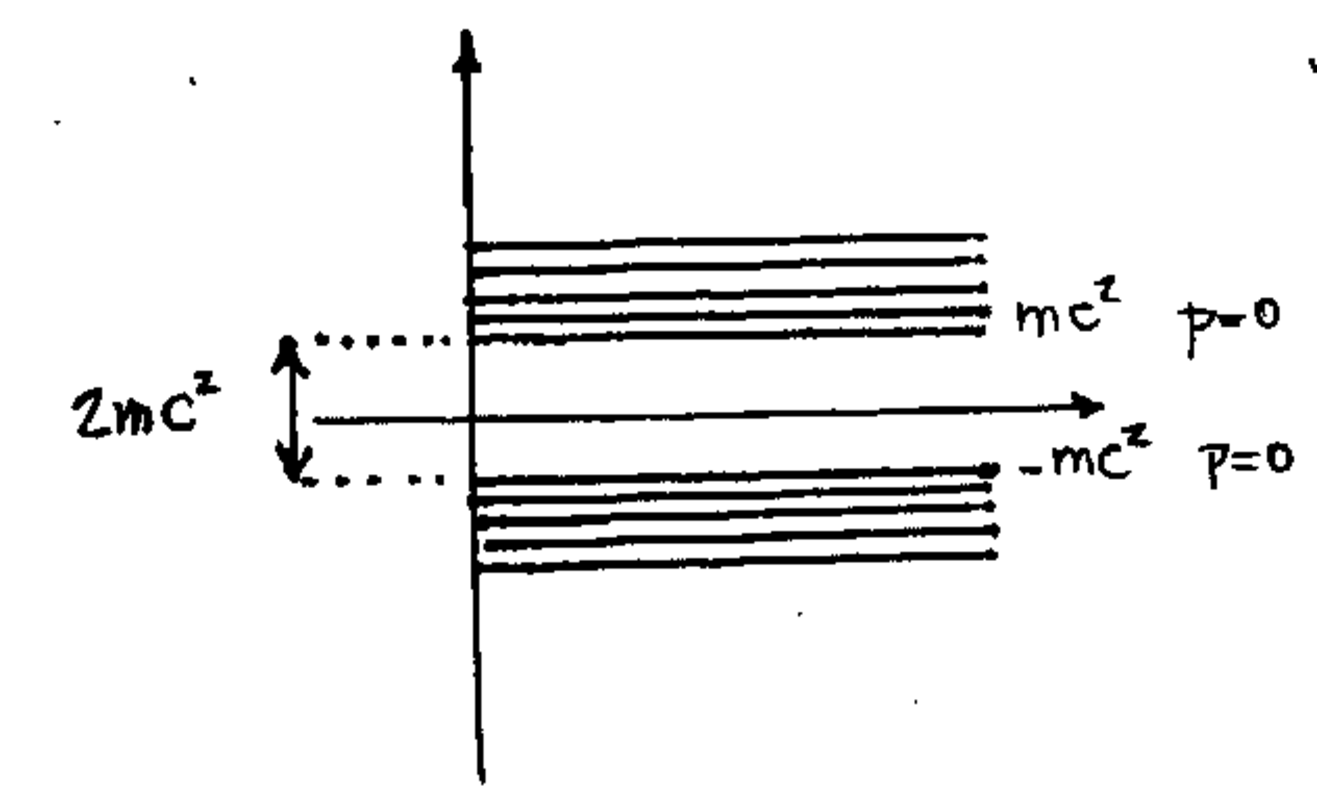
\includegraphics[width=0.6\textwidth]{images/teo2_13.pdf}
	\end{center}
	\caption{}
\end{figure} 

Podemos hacer saltar a la zona positiva una carga $(-e)$ dejando un huevo positivo (equivalente a una carga 
$+e$). Es una creación e pares $\gamma \to e^-e^+$, sin embargo el proceso inverso $ e^-e^+ \to \gamma$ de 
aniquilación de pares ocurre prontamente.
Se observó experimentalmente.

\begin{figure}[htb]
	\begin{center}
	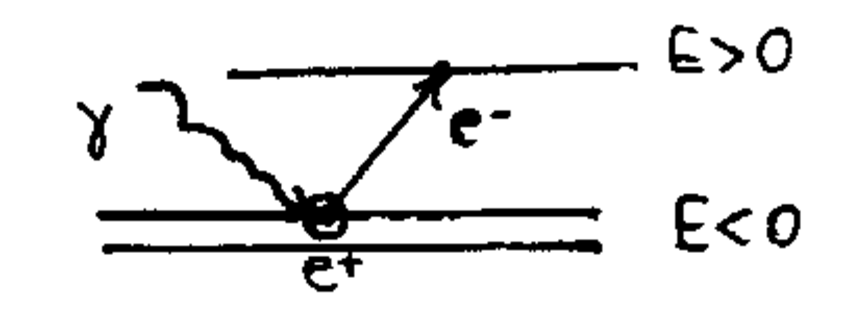
\includegraphics[width=0.6\textwidth]{images/teo2_14.pdf}
	\end{center}
	\caption{}
\end{figure} 


% \bibliographystyle{CBFT-apa-good}	% (uses file "apa-good.bst")
% \bibliography{CBFT.Referencias} % La base de datos bibliográfica

\end{document}

 	
	
	%###########################################################################
	%		FIN DE LOS CAPITULOS DEL CURSO
	%###########################################################################
	
	%##########################	INDICE	########################################
	
% 	La bibliografía se activará al final cuando se comente la de cada chapter
	
% 	\bibliographystyle{plain}	
%	\bibliographystyle{CBFT-apa-good} % (uses file "apa-good.bst")
% 	\bibliography{CBFT.Referencias} % La base de datos bibliográfica
	
	
	
	\end{document}